\documentclass[
  digital,
%  color,
  oneside,
  nosansbold,
  nocolorbold,
  lof,
  lot
]{fithesis4}
\usepackage[resetfonts]{cmap}
\usepackage[T1,T2A]{fontenc}
\usepackage[
  main=english,
  english, german, russian, czech, slovak
]{babel}
\usepackage{paratype}
\def\textrussian#1{{\usefont{T2A}{PTSerif-TLF}{m}{rm}#1}}
\thesissetup{
    date        = \the\year/\the\month/\the\day,
    university  = mu,
    faculty     = sci,
    type        = bc,
    department  = Department of Physical Electronics,
    author      = Tomáš Rottenberg,
    gender      = m,
    programme   = Nanotechnology,
    field       = Physics,
    advisor     = {Mgr. Pavel Ondračka, Ph.D.},
    title       = {Machine learning-assisted atomistic modeling of amorphous materials},
    TeXtitle    = {Machine learning-assisted atomistic modeling of amorphous materials},
    keywords    = {
      machine learning,
      computational physics,
      atomistic modeling,
      molecular dynamics,
      neural networks,
      DeePMD
    },
    TeXkeywords = {
      machine learning,
      computational physics,
      atomistic modeling,
      molecular dynamics,
      neural networks,
      DeePMD
    },
    abstract    = {We explore the methodology of machine learning-assisted molecular dynamics
simulations for quantum chemistry and solid-state physics by using the Deep
Potential Molecular Dynamics (DeePMD) method. Several neural network
potentials with different network architectures and different training data
were trained based on density functional theory calculations of crystalline
and amorphous silicon and used to calculate various material properties, such
as temperature-dependent equilibrium energy, equilibrium volume, bulk modulus,
and coefficient of thermal expansion. The results were compared to
\textit{ab initio} and experimental results, and the performance of the DeepMD
potentials was critically evaluated. 
},
    thanks      = {These are the acknowledgements for my thesis, which can

span multiple paragraphs.
},
    bib         = bib.bib,
    facultyLogo = fithesis-sci,
    assignment  = assignment.pdf,
}
\usepackage{makeidx}
\makeindex
\usepackage[acronym]{glossaries}
\renewcommand*\glspostdescription{\hfill}
\loadglsentries{abbrs.tex}
\makenoidxglossaries
\usepackage{paralist}
\usepackage{amsmath}
\usepackage{mathtools}
\usepackage{physics}
\usepackage[thinc]{esdiff}
\usepackage{amsthm}
\usepackage{amsfonts}
\usepackage{url}
\usepackage{hyperref}
\usepackage{markdown}
\usepackage{listings}
\lstset{
  basicstyle      = \ttfamily,
  identifierstyle = \color{black},
  keywordstyle    = \color{blue},
  keywordstyle    = {[2]\color{cyan}},
  keywordstyle    = {[3]\color{olive}},
  stringstyle     = \color{teal},
  commentstyle    = \itshape\color{magenta},
  breaklines      = true,
}
\usepackage{floatrow}
\floatsetup[table]{capposition=top}
\usepackage[babel]{csquotes}
\listfiles
\begin{document}

\chapter*{Introduction}
\markright{\textsc{Introduction}}
\addcontentsline{toc}{chapter}{Introduction}



\chapter{Molecular Dynamics}

Molecular dynamics simulations is an umbrella term for a class of
computational methods used to model and analyze the physical behavior of
systems of atoms and molecules. MD allows one to monitor the full time
evolution of a system, allowing for deep examination of the dynamics of
atomic-level phenomena that cannot be observed directly.
Computer simulations applied to condensed matter systems began their
development as early as the 1950s, when two of the pillars of molecular
simulation were introduced, namely the Monte Carlo (MC) sampling technique and
the molecular dynamics method. In 1964, the first realistic MD simulation was
developed by Rahman, who came up with a realistic model of liquid Argon.
Rahman used the Lennard–Jones pair-wise additive potential and showed, that
MD simulations with smooth potentials were possible.

Around the same time, Verlet proposed a stable numerical integration
algorithm that is still very popular in modern MD software. We will discuss
the Verlet integration algorithm in further chapters of this thesis. Verlet
also invented a time-saving algorithm, the Verlet neighbour list.

A great leap forward in the MD methology happened in 1971, when Rahman and
Stillinger published an MD study on modeling a realistic system of liquid
water, a system composed of molecules, not just individual atoms. The
significant results of their work prompted a multinational group of scientists
centred around Berendsen at CECAM to try using MD simulations for examining
biomolecules. The first MD simulation of a simple protein was due to Karplus
and collaborators, and appeared shortly after, in 1977. In 2013, the Nobel
Prize for Chemistry was awarded to Warshel, Levitt, and Karplus for their work
on computer simulations in biochemistry, which was built upon the efforts of
many researchers who had previously worked on simulating biomolecules.

Another inportant development took place in 1980. In this year, Anderson
published a paper that described how to extend MD to enable it to sample the
isoenthalpic (constant pressure) ensemble. The standard molecular dynamics
algorithm was designed to simulate the behavior of a system of particles at
constant energy, or in the microcanonical ensemble, because the Newton's
equations of motion conserve energy. It was not straightforward to modify the
MD algorithm to sample systems under different, more experimentally relevant
conditions. Andersen's extensions for sampling the isoenthalpic ensemble
inspired the question of whether it was possible to use MD to sample the
canonical ensemble as well. Nosé, building on Andersen's work, introduced a
new variable that linked the kinetic energy of the atoms to the external
temperature, resulting in dynamics that sample the desired ensemble. This
approach is known as the Nosé–Hoover thermostat, which is often used in a
modified form called the Hoover thermostat.

In 1985, Car and Parrinello published a groundbreaking paper in Physical
Review Letters that described a method for combining MD with density
functional theory (DFT) calculations of electronic structure. This approach
eliminated the need for a potential model, as energy, forces, and stress
could be calculated directly from the electronic structure. The Car–Parrinello
method allowed for the simulation of processes that involve bond formation or
breaking and was the first to demonstrate that it is possible to combine
finite temperature simulations with ground-state electronic structure
calculations. This method also served as a bridge between the simulation
community, which typically has a background in statistical mechanics, and the
solid-state physics and quantum chemistry communities, which focus on
electronic structure calculations at zero temperature.

During the 1980s and 1990s, the use of molecular simulations in condensed
matter research became more widespread, due in part to previous successes in
this field and also to the increasing availability and power of computers.

Modern MD methodology is frequently used to refine the three-dimensional
structures of proteins and other large molecules, to study atomic-level
phenomena that cannot be directly observed, such as thin-film growth and ion
implantation, and to investigate the physical properties of nanotechnological
devices that cannot yet be manufactured. In 2015, for example, MD simulation
has been reported for pharmacophore development and drug design.

\section{Classical Methods}

The classical MD implementation uses the so-called "ball and sticks" model,
where atoms and molecules are treated as soft balls and their bonds are
represented by elastic sticks. The laws of classical mechanics define the
dynamics of the entire system.

Each particle in an MD simulation has its own position vector
$\mathbf{r}_i(t) = (x_i(t), y_i(t), z_i(t))$. A particle usually corresponds
to an atom, although it may represent any simulable entity of interest that
can be conveniently described by an interaction law. By Newton's second law
the motion of each particle must obey the following relation
\begin{equation}
  \mathbf{F}_i = m_i \diff[2]{\mathbf{r}_i}{t},
\end{equation}
where $m_i$ is the mass of $i$-th particle and $\mathbf{F}_i$ is the
force acting upon $i$-th particle. Interaction laws are usually specified by
a potential function $U(\mathbf{r}_1, \dots, \mathbf{r}_N)$, which represents
the potential energy of $N$ interacting particles as a function of their
positions. Given the potential, the force acting upon $i$-th atom is
determined by the gradient with respect to particle displacements
\begin{equation}
  \mathbf{F}_i = - \nabla_{\mathbf{r}_i} U(\mathbf{r}_1, \dots, \mathbf{r}_N)
  = - \left(
    \frac{\partial U}{\partial x_i},
    \frac{\partial U}{\partial y_i},
    \frac{\partial U}{\partial z_i}
  \right).
\end{equation}

Let's briefly talk about the meaning and form of the potential $U$
in MD simulations. Any quantum-chemistry textbook would insist, that in order
to appropriately examine a behavior of molecule, we can't just look at its
individual atoms. The quantum-mechanical lense reveals, that when atoms bond
into molecules, their electron orbitals interact in complex ways, giving rise
to non-trivial molecule orbitals. These electronic clouds that span multiple
atoms then determine molecule's interactions with other particles. This paints
molecules as a very complicated quantum systems, where electrons and nuclei
are interacting together in an intricate manner. It turns out, however, that
to a very good approximation, known as the Born–Oppenheimer adiabatic
approximation and based on the difference in mass between nuclei and
electrons, the electronic and nuclear problems can be separated. According to
this approximation, we can presume that the electron clouds equilibrate
quickly for each instanteneous configuration of the heavy nuclei. The nuclei
then move in the field created by the average electron densities.
This allows us to consider the concept of a potential energy surface, which
controls the movement of the nuclei without taking explicit account of the
electrons. Given the potential energy surface, we may use classical mechanics
to follow the dynamics of the nuclei. Rather than solving the
quantum-mechanical problem, we can solve a classic-mechanical problem, in
which the effect of the electrons on nuclei is expressed by en empirical
potential. It can be very challenging to identify a potential function that
accurately represents an energy surfaces of a system, but doing so greatly
simplifies the computational process. Atomic force field models and the
classical MD are based on empirical potentials with a specific functional
form, representing the physics and chemistry of the systems of
interest. The following equation is an example of such a force field, used in
biosystem simulations
\begin{equation}
\begin{alignedat}{2}
  U(\mathbf{r}_1, \dots, \mathbf{r}_N) = &
  \sum_\text{bonds} \frac{a_i}{2} (l_i - l_{i0})^2
  + \sum_\text{angles} \frac{b_i}{2} (\theta_i - \theta_{i0})^2 \\
  &+ \sum_\text{torsions} \frac{c_i}{2} \left[
    1 + \cos(n \omega_i - \gamma_i)
  \right] \\
  &+ \sum_\text{atom pairs} 4 \varepsilon_{ij} \left[
    \left(\frac{\sigma_{ij}}{r_{ij}}\right)^{12}
    - \left(\frac{\sigma_{ij}}{r_{ij}}\right)^{6}
  \right] \\
  &+ \sum_\text{atom pairs} k \frac{q_i q_j}{r_{ij}}.
\end{alignedat}
\end{equation}
The covalent character of the system is defined by the first three terms of
the system, where the summation indices run over all the bonds, angles and
torsions. In contrast, the last two terms are only defined by atom pairs,
with $q_i q_j$ being the product of their charges and $r_{ij} = |r_i - r_j|$
is the distance between the two atoms in the pair. The first two terms give
energies of deformations of the bond lengths $l_i$ and bond angles $\theta_i$
from their respective equilibrium values $l_{i0}$ and $\theta_{i0}$ with force
constants $a_i$ and $b_i$. These two terms model the correct chemical
structure, but prevent more complicated chemical phenomena like bond breaking.
Rotations around the chemical bond are described by the third therm, which is
priodic with periodicity determined by $n$ and heights of rotational barriers
defined by $c_i$. The forth term represents the van der Waals repulsive and
attractive interatomic forces in the form of the Lennard–Jones 12-6 potential.
The last term is the Coulomb electrostatic potential. Some effects due to
specific environments can be accounted for by properly adjusting partial
charges $q_i$ and effective value of the constant $k$ as well as the van der
Waals parameters $\varepsilon_{ij}$ and $\sigma_{ij}$.

We now have a full mathematical description of the problem at hand. Due to the
many-body nature of the problem, it is out of question to solve it
analytically, thus it has to be discretized and solved numerically with a
computer. First, we need to specify the initial conditions of the system,
that is, the initial positions $\mathbf{r}_{i0}$ and initial velocities
$\mathbf{v}_{i0}$ of the particles in the system. Then we have to use a
numerical integrator to continually make finite time interval steps and find
the successive values of positions $\mathbf{r}_i(t)$ and velocities
$\mathbf{v}_{i}(t)$ in the time evolution of the system. A very popular
numerical integration algorithm is the Verlet algorithm, which gained its
popularity for MD simulations mainly due to its simplicity and stability.
The fundamental equation for this algorithm can be obtained from the Taylor
series expansions of the position vector $\mathbf{r}_i(t)$; the full equation
reads
\begin{equation}
  \mathbf{r}_i (t + \Delta t) \doteq 2 \mathbf{r}_i(t)
    - \mathbf{r}_i(t - \Delta t) + \frac{\mathbf{F}_i(t)}{m_i} \Delta t^2
  \label{eq:verlet}
\end{equation}
Equation \eqref{eq:verlet} is accurate up to terms of the fourth power in
$\Delta t$. Velocities can be calculated from the positions or using
alternative leapfrog or velocity Verlet schemes. Precise trajectories
correspond to the scenario where the integration step size approaches
infinitesimally small values. However, it is preferable to utilize larger time
steps in order to sample larger trajectories. In practical applications, the
time step $\Delta t$ is dictated by the fast motions present within the
simulation.

\section{\textit{Ab Initio} Methods}
In classical molecular dynamics, the forces acting on the atoms are derived
from a potential energy function, which is usually based on empirical or
semi-empirical force fields. These force fields are parameterized using
experimental data or quantum mechanical calculations, and they provide an
approximate description of the interactions between atoms. Classical molecular
dynamics is generally not very accurate because it relies on approximations
and empirical parameters and can't account for dynamical events and quantum
effects such as changes in chemical bonding, the presence of important
noncovalent intermediates and tunnelling of protons or electrons. The changes
in bonding and the existence of intermediates can be accounted for using
first-principles (or \textit{ab initio}) MD. \textit{Ab initio} molecular
dynamics (AIMD) is generally more accurate than classical molecular dynamics
because it directly calculates the electronic structure of the system. This
makes it suitable for studying systems where electronic structure plays a
critical role. AIMD is much more computationally expensive, which limits its
applicability to relatively small systems and short timescales. The forces and
electronic structure are determined by solving the Schrödinger equation,
typically using methods from quantum physics, such as the Hartree-Fock method,
density functional theory (DFT), or other wavefunction-based methods.

\section{Density Functional Theory}
Over the last three decades, density functional theory has emerged as the
leading approach for conducting quantum mechanical simulations of periodic
systems. Recently, it has gained popularity among quantum chemists and has
become extensively employed for simulating energy surfaces in molecular
systems. While its origins can be traced back to the early 1930s, DFT was
formally established in 1964 through two theorems developed by Hohenberg and
Kohn.

Simulating an atomic system from first principles means solving the quantum
many-body problem. If we have $N$ nuclei, we are dealing with a problem of
$N + ZN$ electromagnetically interacting particles. The Hamiltonian of such
problem is
\begin{equation}
\begin{alignedat}{2}
  \hat H = & - \frac{\hbar^2}{2} \sum_i \frac{\nabla^2_{\mathbf{R}_i}}{M_i}
  - \frac{\hbar^2}{2} \sum_i \frac{\nabla^2_{\mathbf{r}_i}}{m_e} \\
  & - \frac{1}{4 \pi \varepsilon_0} \sum_{ij} \frac{e^2 Z_i}{|\mathbf{R}_i - \mathbf{r}_j|}
  + \frac{1}{8 \pi \varepsilon_0} \sum_{i\neq j} \frac{e^2}{|\mathbf{r}_i - \mathbf{r}_j|} \\
  & + \frac{1}{8 \pi \varepsilon_0} \sum_{i \neq j} \frac{e^2 Z_i Z_j}{|\mathbf{R}_i - \mathbf{R}_j|}.
\end{alignedat}
\end{equation}
The mass of the nucleus at $\mathbf{R}_i$ is $M_i$, the electrons hamve mass
$m_e$ and are at $\mathbf{r}_i$. The first term is the kinetic energy operator
for the nuclei, the second for the electrons. The last three terms describe
the Coulomb interaction between electrons and nuclei, between electrons and
other electrons, and between nuclei and other nuclei. It is out of question
to solve this problem exactly, therefore we have to introduce some
approximations, leadin to the formulation of DFT.

Firstly, we observe that the nuclei are much heavier and consequently move
much slower than the electrons. This observation justifies rewriting the
Hamiltonian such that
\begin{equation}
  \label{eq:bo-hamiltonian}
  \hat H = \hat T + \hat V + \hat V_\mathrm{ext}.
\end{equation}
Now $\hat T$ represents only the kinetic energy of the electron gas, as this
approximation assumes the nuclei are effectively frozen at their positions.
The term $\hat V$ now represents the electron-electron interaction only. The
last term $\hat V_\mathrm{ext}$ is due to the potential energy of the
electrons in the (now external) potential of the nuclei. System-specific
information is now entirely given by the term $\hat V_\mathrm{ext}$. This
approximation is called the The Born--Oppenheimer approximation.

The quantum many body problem obtained after the first approximation is much
simpler than the original one, but still far too difficult to solve. To reduce
the equation \eqref{eq:bo-hamiltonian} further, we introduce the two
Hohenberg–-Kohn theorems.

\begin{enumerate}
  \item \textit{There is a one-to-one correspondence between the ground-state
  density $\rho(\mathbf{r})$ of a many-electron system (atom, molecule, solid)
  and the external potential $V_\mathrm{ext}$. An immediate consequence is
  that the ground-state expectation value of any observable $\hat O$ is a
  unique functional of the exact ground-state electron density}
  \begin{equation}
    \mel{\Psi}{\hat O}{\Psi} = O[\rho].
  \end{equation}

  \item \textit{For $\hat O$ being the hamiltonian $\hat H$, the ground-state
  total energy functional $H[\rho] \equiv E_{V_\mathrm{ext}}[\rho]$ is of the
  form}
  \begin{equation}
  \begin{alignedat}{2}
    E_{V_\mathrm{ext}}[\rho]
    &= \mel{\Psi}{\hat T + \hat V}{\Psi}
    + \mel{\Psi}{\hat V_\mathrm{ext}}{\Psi} \\
    &= F_{HK}[\rho] +
    \int \rho(\mathbf{r}) V_\mathrm{ext}(\mathbf{r}) \, \mathrm{d}\mathbf{r},
    \label{eq:hk-2}
  \end{alignedat}
  \end{equation}
  \textit{where the Hohenberg-Kohn density functional $F_{HK}[\rho]$ is
  universal for any many-electron system. $E_{V_\mathrm{ext}}[\rho]$ reaches its
  minimal value (equal to the ground-state total energy) for the ground-state
  density corresponding to $V_\mathrm{ext}$.}
\end{enumerate}

Let's pause and ponder the meaning of these theorems for a bit. Each
many-electron system has a unique potential, and each system as a whole is
represented by a unique ground-state many particle wave function, as governed
by the hamiltonian \eqref{eq:bo-hamiltonian} and the Schrödinger equation.
From this wavefunction, we can obtain the corresponding electron density using
the density operator $\hat \rho$ which is defined as
\begin{equation}
  \hat \rho(\mathbf{r}) = \sum_i^N \delta(\mathbf{r}_i - \mathbf{r}).
\end{equation}
The first theorem of Hohenberg–-Kohn tells us, that there exists a one-to-one
correspondence between the ground-state density and the external potential.
The density contains as much information as the wave function does, meaning
all observables can be retrieved from the density only and can be written as
functionals of the density.

The equation \label{eq:hk-2} suggests, that the energy contribution from the
external potential can easily be calculated, given the density function
$\rho(\mathbf{r})$. An explicit expression for $F_{HK}$ is not known,
however, since the term is not dependent on the information of the nuclei and
their position, it is a universal functional for any many-electron system and
can be found. Moreover, the second theorem states that the ground-state
density $\rho$ corresponding to the external potential
$V_\mathrm{ext}(\mathbf{r})$ minimizes the total energy functional
$E_{V_\mathrm{ext}}[\rho]$, which allows us to use the variational principle
of Rayleigh--Ritz in order to find the ground-state density.

Noting once again, that the the Hohenberg--Kohn functional $F_{HK}$ is only
dependent on the electron structur and not on the structure of the nuclei, we
can now proceed with finding an expression for $F_{HK}$. There exist several
options for defining the energy of the electron many-body system. The exact
solution is simply
\begin{equation}
  E_e = T + V,
\end{equation}
where $T$ and $V$ are the exact kinetic and electron-electron potential energy
functionals. The Hartree--Fock solution is defined as
\begin{equation}
  E_{HF} = T_0 + \underbrace{(V_H + V_x)}_V,
\end{equation}
where $T_0$ is the functional for the kinetic energy of a non-interacting
electron gas, $V_H$ stands for Hartree contribution and $V_x$ for exchange
contribution. There's also the Hartree solution, which lacks the exchange
contribution
\begin{equation}
  E_H = T0 + V_H.
\end{equation}
We use this solution as a definition for the exchange energy
\begin{equation}
  V_x = E_{HF} - E_H = V - V_H.
\end{equation}
We define the correlation energy as the difference between the
exact solution and the Hartree--Fock solution
\begin{equation}
  V_c = E_e - E_{HF} = T - T_0.
\end{equation}
We can now rewrite the Hohenberg--Kohn functional
\begin{equation}
\begin{alignedat}{2}
  F_{HK} &= T + V + T_0 - T_0 \\
  &= T_0 + V + \underbrace{(T - T_0)}_{V_c} \\
  &= T_0 + V + V_c + V_H - V_H \\
  &= T_0 + V_H + V_c + \underbrace{(V - V_H)}_{V_x} \\
  &= T_0 + V_H + \underbrace{(V_x + V_c)}_{V_{xc}}.
\end{alignedat}
\end{equation}
The term $V_{xc}$ is called the exchange--correlation energy functional. We
can write the energy functional explicitly as
\begin{equation}
  E_{V_\mathrm{ext}}[\rho] = T_0[\rho] + V_H[\rho] + V_{xc}[\rho]
  + V_{ext}[\rho].
\end{equation}
The rewritten energy functional can be interpreted as an energy functional of
a non-interacting classical electron gas, subject to the potential due to the
nuclei and to the potential due to exchange and correlation effects. This is
how the Kohn--Sham Hamiltonian is defined
\begin{equation}
\begin{alignedat}{2}
  \hat H_{KS} &= \hat T_0 + \hat V_H + \hat V_{xc} + \hat V_{ext} \\
  &= -\frac{\hbar^2}{2 m_e} \nabla_i^2
  + \frac{e^2}{4 \pi \varepsilon_0} \int
  \frac{\rho(\mathbf{r})}{|\mathbf{r} - \mathbf{r}_i|} \, \mathrm{d}\mathbf{r}
  + \hat V_{xc} + \hat V_{ext}.
\end{alignedat}
\end{equation}
The exchange-correlation potential is given by the functional derivative
\begin{equation}
  \hat V_{xc} = \frac{\delta V_{xc}[\rho]}{\delta \rho}.
\end{equation}
The theorem of Kohn and Sham can now be formulated as follows:
\begin{displayquote}
  \textit{
    The exact ground-state density $\rho(\mathbf{r})$ of an N-electron system
    is
  }
  \begin{equation}
    \rho(\mathbf{r}) = \sum_{i=1}^N \phi_i(\mathbf{r})^* \phi_i(\mathbf{r}),
  \end{equation}
  \textit{
    where the single-particle wave functions $\phi_i(\mathbf{r})$ are the $N$
    lowest-energy solutions of the Kohn-Sham equation
  }
  \begin{equation}
    \hat H_{KS} \phi_i = \varepsilon_i \phi_i.
  \end{equation}
\end{displayquote}
This theorem enables us to recover the ground-state density by solving $N$
Schrödinger-like equations for non-interacting single particles as opposed to
solving conventional Schrödinger equation for system of $N$ interacting
electrons, which would require us to resolve a complex system of coupled
differential equations. It is important to note, however, that the
single-particle wave functions $\phi_i(\mathbf{r})$ are not the wave functions
of electrons and they do not have any physical meaning -- they are only
mathematical artifacts. Only the resultant ground-state density
$\rho(\mathbf{r})$ is physically relevant.

Both the Hartree operator $V_H$ and the exchange-correlation operator $V_{xc}$
depend on the density $\rho(\mathbf{r})$, which in turn depends on the
$\phi_i$ which are being searched. However, we can't write down and solve the
equations for $\phi_i$, until we know the density $\rho(\mathbf{r})$. This
chicken and egg scenario is known as the self-consistency problem and requires
an iterative procedure with an initial guess of the density function to escape
from this paradox. The process is further described in figure
\ref{fig:self-consistency}.

\begin{figure}
  \begin{center}
    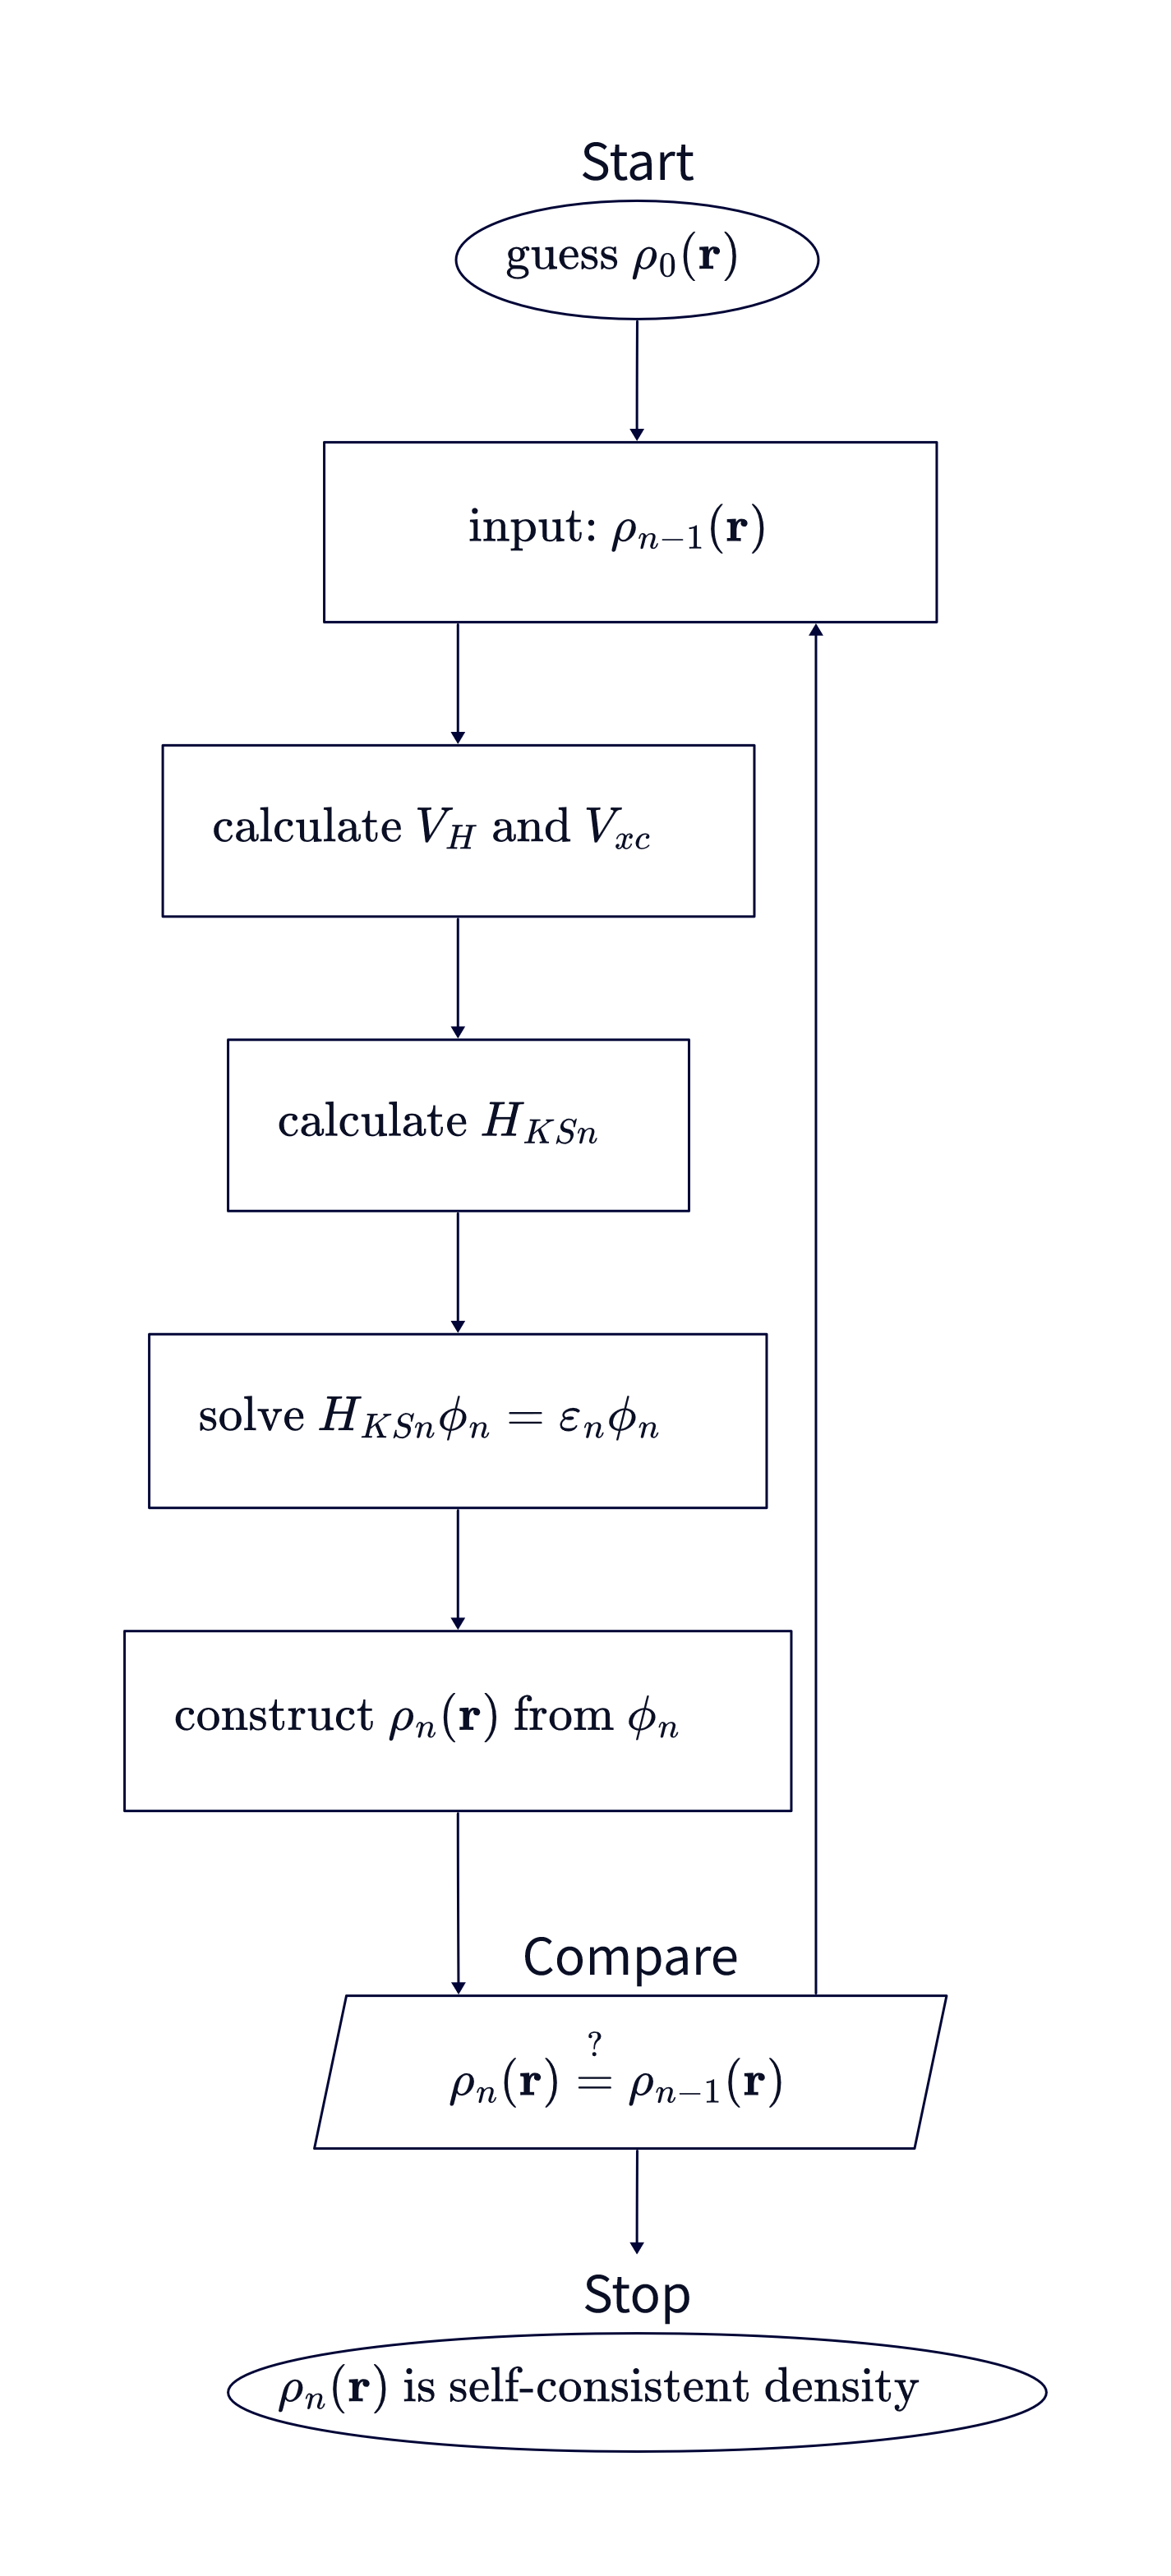
\includegraphics[width=7.3cm]{asset/self_consistency}
  \end{center}
  \caption{Flowchart for solving the self-consistent DFT problem.}
  \label{fig:self-consistency}
\end{figure}

\section{Machine Learning}

Until recently, classical molecular dynamics simulations based on empirical
force fields and \textit{ab initio} calculations were the only available
methods in computational physicists' toolbox. However, the rapid advent of
machine learning and artificial intelligence algorithms drastically changed
the landscape of physical simulations. When trained on large datasets of
atomic configurations and corresponding potential energies and forces,
ML models can reproduce the original data accurately, while still retaining
the linearly scaling computational cost of classical MD simulations. Although
ML methods are often quite data hungry, their accuracy, scalability, and
transferability make them a very attractive alternative for various MD
applications.

\section{Deep Potential Molecular Dynamics}

The Deep Potential Molecular Dynamics (DeepMD) \parencite{Zhang_2018} method
uses neural networks for modeling many-body potentials and interatomic forces
to drive classical molecular dynamics. The neural network architectures used
by the DeepMD method are designed so that they preserve all the natural
symmetries in the problem. These models are trained on \textit{ab initio} data
and are capable of producing results that are essentially indistinguishable
from the original data while scaling linearly with the system size.

One of the most notable challenges in developing an efficient NN schema for
molecular dynamics is devising an input format that would preserve the
translational, rotational, and permutational symmetry of the system. The raw
atomic coordinates from MD simulations cannot be used directly, as they do not
exhibit these symmetries. Different ML models were proposed to address this
problem. For example, the Behler--Parrinello neural network (BPNN)
\parencite{PhysRevLett.98.146401} maps the coordinates onto a large set of
two- and three-body symmetry functions. Another proposed model,
gradient-domain machine learning (GDML)
\parencite{doi:10.1126/sciadv.1603015}, maps the coordinates onto the
eigenvalues of the Coulomb matrix. Both of these protocols are successful, but
they are also needlessly complicated, with their use-cases being rather
limited, as they do not come from a first-principles analysis of the modeling
problem, and it is not straightforward to extend them beyond simple systems.
The DeepMD methodology attempts to provide a more first principle-based
approach to overcome the limitations associated with auxiliary quantities like
the symmetry functions or the Coulomb matrix.

Consider a system of $N$ atoms, where the coordinates of these atoms can be
represented as a set of position vectors
$\{\mathbf{R}_1, \dots, \mathbf{R}_N\}$, with each
$\mathbf{R}_i \in \mathbb{R}^3$. DeepMD decomposes the total system energy $E$
into a sum of energy contributions from individual atoms,
\begin{equation}
  E = \sum_i^N E_i,
\end{equation}
where $i$ is an index of an individual atom. Atomic energy $E_i$ is fully
determined by the position of the $i$th atom and by the positions of its near
neighbours,
\begin{equation}
  E_i = E_{s(i)}(\mathbf{R}_i, \{\mathbf{R}_j \mid j \in  N_{R_C}(i)\}),
\end{equation}
where $N_{R_C}(i)$ denotes the index set of the neighbour atoms of atom $i$
within the cut-off radius $R_C$. $s(i)$ is the chemical species of atom $i$.
For reasons discussed above, it is less than optimal to use the position
vector data $\mathbf{R}_i, \{\mathbf{R}_j \mid j \in  N_{R_C}(i)\}$ when
modeling the function $E_{s(i)}$ with DNN. Thus, the DeepMD method introduces
a mapping from position vectors to "descriptors" of atomic chemical
environment, that better capture the underlying symmetries.

To construct the descriptor for atom $i$, we first calculate the relative
positions of its neighbouring atoms,
\begin{equation}
  \mathbf{R}_{ij} = \mathbf{R}_j - \mathbf{R}_i.
\end{equation}
The coordinate of the relative position $R_{ij}$ under the lab reference frame
$\{\mathbf{e}_x^0, \mathbf{e}_y^0, \mathbf{e}_z^0\}$ is denoted by
$(x_{ij}^0, y_{ij}^0, z_{ij}^0)$, such that
\begin{equation}
  \mathbf{R}_{ij} = x_{ij}^0 \mathbf{e}_x^0 + y_{ij}^0 \mathbf{e}_y^0
    + z_{ij}^0 \mathbf{e}_z^0.
\end{equation}
Both representations $\mathbf{R}_{ij}$ and $(x_{ij}^0, y_{ij}^0, z_{ij}^0)$
preserve the translational symmetry. The rotational symmetry is captured by
constructing a local frame of reference and using it to express the
coordinates of neighbouring atoms. We first pick atoms with indices $a(i)$ and
$b(i)$ from the neighbours $N_{R_C}(i)$ by certain user-specified rules. The
local reference frame $\{\mathbf{e}_{i1}, \mathbf{e}_{i2}, \mathbf{e}_{i3} \}$
of atom $i$ is then constructed by
\begin{align}
  \mathbf{e}_{i1} = \mathbf{e}(\mathbf{R}_{ia(i)}), \\
  \mathbf{e}_{i2} = \mathbf{e}\left(
    \mathbf{R}_{ib(i)} -
    (\mathbf{R}_{i b(i)} \cdot \mathbf{e}_{i1}) \mathbf{e}_{i1}
  \right), \\
  \mathbf{e}_{i3} = \mathbf{e}_{i1} \times \mathbf{e}_{i2},
\end{align}
where $\mathbf{e}(\mathbf{R})$ denotes the normalized vector of $\mathbf{R}$,
such that $\mathbf{e}(\mathbf{R}) = \mathbf{R} / |\mathbf{R}|$. The local
coordinate $(x_{ij}, y_{ij}, z_{ij})$ is then calculated from the lab
coordinate $(x_{ij}^0, y_{ij}^0, z_{ij}^0)$ through the transformation
\begin{equation}
  (x_{ij}, y_{ij}, z_{ij}) = (x_{ij}^0, y_{ij}^0, z_{ij}^0) \cdot
    \mathcal{R}(\mathbf{R}_{i a(i)}, \mathbf{R}_{i b(i)}),
\end{equation}
where
\begin{equation}
  \mathcal{R}(\mathbf{R}_{i a(i)}, \mathbf{R}_{i b(i)}) =
    [\mathbf{e}_{i1}, \mathbf{e}_{i2}, \mathbf{e}_{i3}]
\end{equation}
is the rotation matrix with the columns being the local reference frame
vectors. The descriptive information of atom $i$ given by neighboring atom $j$
is then obtained by using either both the radial and angular information or
only the radial information
\begin{equation}
  \{D_{ij}\} = \begin{cases}
    \left\{
      \frac{1}{R_{ij}},
      \frac{x_{ij}}{R_{ij}},
      \frac{y_{ij}}{R_{ij}},
      \frac{z_{ij}}{R_{ij}}
    \right\}, & \text{full information;} \\
    \left\{\frac{1}{R_{ij}}\right\}, & \text{radial-only information.}
  \end{cases}
  \label{eq:descriptor}
\end{equation}
The order of the neighbour indices $j$ in $\{D_{ij}\}$ is fixed by sorting
them first by their chemical species and then, within each chemical species,
according to their inverse distances to the atom $i$, i.e., $1/R_{ij}$. The
permutational symmetry is naturally preserved in this way. This is the full
procedure for constructing the mapping from atomic positions to descriptors,
which is denoted by
\begin{equation}
  \mathbf{D}_i = \mathbf{D}_i(
    \mathbf{R}_i, \{\mathbf{R}_j \mid j \in  N_{R_C}(i)\}
  ).
\end{equation}
The descriptors $\mathbf{D}_i$ preserve the translational, rotational, and
permutational symmetries and are passed to a DNN to evaluate the atomic
energies. This process can be mathematically expressed as
\begin{equation}
  E_{s(i)} = \mathcal{N}_{s(i)}(\mathbf{D}_{i}),
  \label{eq:dnn}
\end{equation}
The DNN used by DeepMD method is a feed forward neural network with multiple
hidden layers, where each layer transforms the input data $\mathbf{d}_i^{p-1}$
from the previous layer into $\mathbf{d}_i^{p}$ and passes them as an input
to the next layer. The transformation consists of a linear and a non-linear
step, i.e.
\begin{equation}
  \mathbf{d}_{i}^{p} = \varphi \left(
    \mathbf{W}_{s(i)}^p \mathbf{d}_i^{p-1} + \mathbf{b}^p_{s(i)}
  \right),
\end{equation}
where $\varphi$ represents the non-linear function and $\mathbf{W}_{s(i)}^p$
and $\mathbf{b}^p_{s(i)}$ are free parameters of the linear transformation to
be optimize by the training process. In order to determine the unknown
parameters ${\mathbf{W}{s}^p, \mathbf{b}s^p}$ of the linear transformation, a
loss function $L$ is minimized during the training process. This loss
function is calculated by taking a weighted sum of mean square errors of the
predictions made by the DNN. Specifically, the loss function
$L(p\epsilon, p_f, p\xi)$ is defined as follows:
\begin{equation}
  L(p_\epsilon, p_f, p_\xi) = \frac{p_\epsilon}{N} \Delta E^2 +
  \frac{p_f}{3N} \sum_i |\Delta \mathbf{F}_i|^2
  + \frac{p_\xi}{9N} ||\Delta \Xi||^2,
\end{equation}
where $\Delta E$, $\Delta \mathbf{F}_i$ and $\Delta \Xi$ denote root mean
square (RMS) error in energy, force, and virial, respectively. The weights
$p_\epsilon$, $p_f$ and $p_\xi$ are varying during the learning process. Their
dependence on the learning step $t$ is defined as
\begin{equation}
  p(t) = p^\text{limit} \left[1 - \frac{r_l(t)}{r_l^0}\right]
  + p^\text{start} \left[\frac{r_l(t)}{r_l^0}\right],
  \label{eq:loss-weight}
\end{equation}
where $r_l(t)$ and $r_l^0$ are the learning rate at training step $t$ and the
learning rate ate the beginning, respectively. The prefactors $p^\text{limit}$
and $p^\text{start}$ are specified by the user configuration. It is easy to
observe that as the learning process starts the factor $\frac{r_l(t)}{r_l^0}$
tends to $1$ and thus the value of $p(t)$ tends to $p^\text{start}$. When the
learning process ends, the factor $1 - \frac{r_l(t)}{r_l^0}$ tends to $1$ and
thus the value of $p(t)$ tends to $p^\text{limit}$. By tuning these
parameters a user can precisely specify what physical properties of the system
should the model be learning to predict at different stages of the learning
process. The learning rate $r_l(t)$ function is in our case given by
\begin{equation}
  r_l(t) = r_l^0 \cdot d_r^{t/d_s},
  \label{eq:learning-rate}
\end{equation}
where $d_r$ and $d_s$ are the decay rate and decay steps, respectively. The
decay rate $d_r$ is required to be less than 1.

\chapter{Equations of State}

Equations of state (EOS) represent thermodynamic relationships between state
variables that characterize the condition of matter under specific physical
parameters, including pressure, volume, temperature, and internal energy.
State equations usually take the form of
\begin{equation}
  f(p, V, T) = 0,
\end{equation}
where $p$ is the pressure, $V$ is the volume, and $T$ the temperature of the
system. There exists no single equation of state that would accurately
predict the properties of all systems under all possible conditions. As a
consequence, a vide variery of state equations have been developed over the
years, each modelling a specific class of materials under specific conditions.
When modelling a specific system using a particular state equation, it is
important to carefully consider the limits of its applicability and its
suitability for the system of interest.

\section{Birch--Murnaghan Equation of State}

The Birch-Murnaghan EOS is an empirical isotropic equation that describes the
relationship between the volume, pressure, and energy of a solid material
under compression. Developed by Francis Birch in 1947, it is based on the
Murnaghan equation of state and is widely used in solid-state physics,
materials science, and geophysics to examine materials under high pressure
conditions.

The derivation of the Birch--Murnaghan EOS is based on the Eulerian finite
strain theory. When strains are infinitesimal, the dimensions of a body
decrease linearly with pressure. However, this is not the case when strains
are finite because matter becomes increasingly incompressible with pressure.
The Eulerian finite elastic strain theory treats this phenomenon. When
introducing the Eulerian scheme, it is important to note the following points:
\begin{itemize}
  \item Unlike the Lagrangian scheme, which uses the pre-compression state as
  a reference, the Eulerian scheme uses the post-compression state.
  \item Changes are expanded in squared length before and after compression.
\end{itemize}

We start by considering a cube of side $x_0$ and volume $V_0 = x_0^3$. We
apply a compression $u$ ($u < 0$), so that the length of the side becomes
$x = x_0 + u$. The change in squared length is expressed as
\begin{equation}
  x^2 - x_0^2 = x^2 - (x - u)^2 = 2ux - u^2.
\end{equation}
The displacement $u$ under uniform compression should be proportional to the
length of the cube's side with a proportionality constant $c$
\begin{equation}
  u = cx.
\end{equation}
The constant $c$ is referred to as the strain in the linear elasticity.
Combining the above equations we get
\begin{equation}
  x^2 - x_0^2 = 2cx^2 - c^2x^2 = 2x^2(c - \frac{1}{2}c^2).
\end{equation}
We obtain the definition for the second-power Eulerian finite strain
\begin{equation}
  \varepsilon_{E2} = c - \frac{1}{2}c^2.
\end{equation}
We can use the Eulerian finite strain to express the change in squared length
of the side of the cube as
\begin{equation}
  x^2 - x_0^2 = 2\varepsilon_{E2}x^2.
\end{equation}
The ration of the pre-compression side length to the post-compression side
length can be expressed using the Eulerian finite strain as
\begin{equation}
  \frac{x_0}{x} = \sqrt{1 - 2\varepsilon_{E2}}.
\end{equation}
We can use this equation to also express the ratio of the pre-compression
volume and the post-compression volume as
\begin{equation}
  \frac{V_0}{V} = \left(\frac{x_0}{x}\right)^3 =
  \left(1 - 2 \varepsilon_{E2}\right)^{\frac{3}{2}}.
\end{equation}
Conversely, we can express the finite strain using the volume ratio
\begin{equation}
  \varepsilon_{E2} = \frac{1}{2} \left[
    1 - \left(\frac{V_0}{V}\right)^{\frac{3}{2}}
  \right].
\end{equation}
The $\varepsilon_{E2}$ when the body is compressed. To make the strain
positive, we define $f_{E2}$ as
\begin{equation}
  f_{E2} = -\varepsilon_{E2} = \frac{1}{2} \left[
    \left(\frac{V_0}{V}\right)^{\frac{3}{2}} - 1
  \right].
  \label{eq:finite-strain}
\end{equation}
The first law of thermodynamics in terms of Helmholtz free energy is given by
\begin{equation}
  \mathrm{d}F = - S \mathrm{d}T - p \mathrm{d}V.
\end{equation}
We can simply derive an expression for pressure of isothermal system as
\begin{equation}
  p = - \left(\frac{\partial F}{\partial V}\right)_T.
  \label{eq:isothermal-pressure}
\end{equation}
The Helmholtz free energy of matter may be expressed by a series of the
Eulerian finite strain
\begin{equation}
  F = a_0 + a_1 f_{E2} + a_2 f_{E2}^2 + a_3 f_{E2}^3 + \cdots.
\end{equation}
The absolute value of $F$ is abitrary, so we can set $a_0 = 0$. Pressure
should be zero in an uncompressed state, as should $f_{E2}$, so from the
equation \eqref{eq:isothermal-pressure} we get
\begin{equation}
  p_{f_{E2}=0} = - \left(
    \frac{\partial F}{\partial f_{E2}}
  \right)_{T,f_{E2}=0} \left(
    \frac{\partial f_{E2}}{\partial V}
  \right)_{T, f_{E2}=0} = -a_1 \left(
    \frac{\partial f_{E2}}{\partial V}
  \right)_{T, f_{E2}=0} = 0.
\end{equation}
Therefore coefficient $a_1$ in the expansion of $F$ is $a_1 = 0$. We continue
by truncating the expansion to
\begin{equation}
  F \doteq a_2 f_{E2}^2 + a_3 f_{E2}^3.
\end{equation}
Plugging this into the equation \eqref{eq:isothermal-pressure}, we get
\begin{equation}
\begin{alignedat}{2}
  p &= -\left[
    \frac{\partial}{\partial V}(a_2 f_{E2}^2 + a_3 f_{E2}^3)
  \right]_T \\
  &= - (2 a_2 f_{E2} + 3 a_3 f_{E2}^2)
  \left( \frac{\partial f_{E2}}{\partial V}\right)_T \\
  &= -2 a_2 (1 + \xi_1 f_{E2}) f_{E2} \left(
    \frac{\partial f_{E2}}{\partial V}
  \right)_T,
  \label{eq:pressure}
\end{alignedat}
\end{equation}
where $\xi_1 = 3 a_3/2 a_2$. As derived in \cite{min9120745}, the parameter
$\xi_1$ is given by
\begin{equation}
  \xi_1 = \frac{3}{2}\left(B_{T_0}' - 4\right),
  \label{eqn:xi_1}
\end{equation}
where $B_{T_0}'$ is the pressure derivative of the isothermal bulk modulus at
standard temperature. Refferring to the same paper, the coefficient $a_2$ is
\begin{equation}
  a_2 = \frac{9}{2} B_{T_0} V_0,
  \label{eqn:a_2}
\end{equation}
where $B_{T_0}$ is the isothermal bulk modulus at standard temperature. From
definition of finite strain we get
\begin{equation}
  \left(\frac{\partial f_{E2}}{\partial V}\right)_T = - \frac{1}{3 V_0} \left(
    \frac{V_0}{V}
  \right)^{\frac{5}{3}}.
  \label{eq:finite-strain-derivative}
\end{equation}
By plugging equations \eqref{eq:finite-strain},
\eqref{eq:finite-strain-derivative}, \eqref{eqn:a_2}, \eqref{eqn:xi_1} into
\eqref{eq:pressure}, we recover the the third-order Birch--Murnaghan EOS of
the form
\begin{equation}
  \small{p = \frac{3}{2} K_{T_0} \left[
    \left(\frac{V_0}{V}\right)^{\frac{7}{3}}
    - \left(\frac{V_0}{V}\right)^{\frac{5}{3}}
  \right] \left[
    1 + \frac{3}{4}(B_{T_0}' - 4)\left\{
      \left(\frac{V_0}{V}\right)^{\frac{2}{3}} - 1
    \right\}
  \right].}
\end{equation}

\chapter{Implementation and Methodology}

The implementation of the DeepMD protocol employed in this thesis is based on
the DeepMD-kit software suite \cite{Wang_DeePMD-kit_A_deep_2018}. DeepMD-kit
uses TensorFlow \cite{tensorflow2015-whitepaper} to provide an efficient and
flexible toolkit for utilizing the DeepMD scheme. DeepMD-kit comes with an
interface to the LAMMPS classical molecular dynamics code \cite{LAMMPS},
which was used in this work for computing all the material properties with the
trained machine learning models. The models were trained on MD data generated
with OpenMX, DFT pseudo-potential code with a numerical atomic basis set
\footnote{
    See \url{https://www.openmx-square.org/}
}. The Python programming language
\footnote{
    See \url{https://www.python.org/}
}, along with its multitude of scientific computation packages, was used for
building the training and evaluation infrastructure. All of the code needed to
reproduce the results presented in this thesis is available online
\footnote{
    See \url{https://github.com/hacksparr0w/bachelor-thesis}
}.

\section{Preparing the DFT Datasets}

As already stated, all AIMD trajectories were calculated using OpenMX. Since
the computation resources available for this work were quite limited, we
chose to only work with simple systems of pure silicon, as they do not
exhibit any complicated quantum mechanical effects and thus should be easier to model and
train on. To see how well the models perform on a wide variety of learning
data, three distinct datasets were prepared: an amorphous silicon dataset, a
crystalline silicon dataset, and a mixed dataset containing both the amorphous
and the crystalline frames. Each dataset contains a selection of frames taken
from OpenMX simulations of silicon systems with different volumes. After the
simulation frames were generated, they were further distilled down so as not
to include frames that were too similar to each other. This was done simply by
removing frames that were too close to each other in terms of their time step
(every 10th frame was selected). The detailed parameters for each used dataset
are listed in table \ref{tab:datasets}. The DFT training data consisted of
crystalline system trajectories with 1000 steps run at a temperature of 1500 K
and amorphous system trajectories that were generated by first running 500
steps at a temperature of 4000 K and then cooling the system down to 300 K in
another 1000 steps. The systems were generated on a $3 \times 3 \times 3$
$k$-grid (27 $k$-points) with an energy cutoff of $250 \, \mathrm{Ry}$ and
using the PBE functional \cite{PhysRevLett.77.3865}.

\begin{table}
  \begin{tabularx}{\textwidth}{lllll}
    \toprule
    \multicolumn{1}{c}{} & \multicolumn{2}{c}{Training} & \multicolumn{2}{c}{Validation} \\
    Dataset & Samples & Frames & Samples & Frames \\
    \midrule
    Crystalline & c-0.99 & 200 & c-1.01 & 200 \\
     & c-1.03 & 200 & & \\
    \midrule
    Amorphous & a-2.15 & 150 & a-2.25 & 150 \\
     & a-2.20 & 150 & a-2.31 & 150 \\
     & a-2.29 & 150 & & \\
     & a-2.30 & 150 & & \\
     & a-2.35 & 150 & & \\
     & a-2.40 & 150 & & \\
    \midrule
    Combined & c-0.99 & 200 & c-1.01 & 200 \\
     & c-1.03 & 200 & & \\
     & a-2.15 & 150 & a-2.25 & 150 \\
     & a-2.20 & 150 & a-2.31 & 150 \\
     & a-2.29 & 150 & & \\
     & a-2.30 & 150 & & \\
     & a-2.35 & 150 & & \\
     & a-2.40 & 150 & & \\
    \bottomrule
  \end{tabularx}
  \caption{Overview of the DFT training datasets.}
  \label{tab:datasets}
\end{table}

\section{Choosing the DNN Hyperparameters}

DeepMD provides a bright palette of hyperparameters that can be used to
fine-tune the behavior of a DNN. The following is an excerpt from a sample DNN
training input:

\shorthandoff{-}
\begin{markdown*}{%
  hybrid,
  definitionLists,
  footnotes,
  inlineFootnotes,
  hashEnumerators,
  fencedCode,
  citations,
  citationNbsps,
  pipeTables,
  tableCaptions,
}
```
{
  "model": {
    "descriptor": {
      "type": "se_e2_a",
      "sel": [70],
      "rcut_smth": 1.8,
      "rcut": 6.0,
      "neuron": [5, 10, 20],
      "resnet_dt": false,
      "seed": 260222622
    },
    "fitting_net": {
      "neuron": [20, 20, 20],
      "resnet_dt": true,
      "seed": 260222622
    }
  },
  "learning_rate": {
    "type":"exp",
    "decay_steps": 20000,
    "start_lr": 0.001,
    "stop_lr": 1e-08
  },
  "loss": {
    "type": "ener",
    "start_pref_e": 1,
    "limit_pref_e": 500,
    "start_pref_f": 1000,
    "limit_pref_f": 10,
    "start_pref_v": 0,
    "limit_pref_v": 0
  },
  "training": {
    "numb_steps": 2000000,
    "seed": 10
  }
}
```
\end{markdown*}
\shorthandon{-}
\noindent Let's briefly discuss the most important configuration parameters
and their effect on the training and inference processes.

The \texttt{model} configuration section defines the architecture details of
a DNN. As per the definition in \eqref{eq:dnn}, the neural network is simply a
function of descriptors that predicts an energy value. The DeepMD
protocol implements this function as two separate neural networks,
where one is called the descriptor network and is defined by the
\texttt{model.descriptor} configuration section, and the other is called the
fitting network and is defined by the \texttt{model.fitting\_net}
configuration section. The descriptor network is fed with the descriptor data
as specified by the \texttt{model.descriptor.type} option, which makes it
possible to control whether the network uses the full radial and angular
information as per \eqref{eq:descriptor}. All of the models trained in this
work use full radial and angular information, so the
\texttt{model.descriptor.type} option is always set to \texttt{se\_e2\_a}.
The \texttt{model.descriptor.sel} option determines how many neighboring atoms
for a given atom type (indices correspond to the indices of the
\texttt{model.descriptor.type} option) are used for inference. The ideal value
for this option can be determined empirically from the training data using the
\texttt{dp neighbor-stat} utility that comes with the DeepMD-kit software.
This value was kept constant for all models in this work. The cutoff radius
specified by the \texttt{model.descriptor.rcut} and
\texttt{model.descriptor.rcut\_smth} options limits the radius of the local
environment constructed for each atom. The neighbors filtered with the
\texttt{model.descriptor.sel} option must be within the cutoff radius, which
is measured in \AA. The most important hyperparameters that have perhaps the
most significant effect on the quality of the model inference are
the \texttt{model.descriptor.neuron} and \texttt{model.fitting\_net.neuron}
options. These options specify the number of layers and the number of neurons
in each layer of the neural network. One of the difficulties of using deep neural
networks is coming up with good heuristics for driving the decisions on the
appropriate network architectures. A great portion of
\autoref{chap:results-and-evaluation} focuses on choosing and evaluating
various network architectures. When training the models, it is important to
choose a random seed that is used by the internal pseudo-random number
generator to initialize the weights and biases of the neural network. This is
very important for two reasons. Firstly, we can ensure the reproducibility of
training results by using the same seeds. Secondly, we can train multiple
models with different seeds and estimate uncertainties based on their
predictions differences, which will differ more the more uncertain the models
are. A comparison of models with different seeds is also discussed in later
chapters.

Another important configuration section is the \texttt{learning\_rate}
section. It implements the learning rate function as per
\eqref{eq:learning-rate}. The values of this configuration were optimized to
go along with the empirically chosen number of training steps
(the \texttt{training.numb\_steps} option) and do not differ on a per-model
basis.

Last but not least, the \texttt{loss} configuration section defines the
behavior of the loss function by varying the loss prefactors defined in
\eqref{eq:loss-weight}. In our case, the loss function is set so that it
aggressively optimizes for the force predictions at the beginning of the
training process and then gradually shifts the focus to the energy
predictions.

The whole training matrix of models used in this work is available in table
\ref{tab:models}. All of the trained models were evaluated using the
\texttt{dp test} utility ran on one of the systems from the validation
dataset.

\begin{table}
  \begin{tabularx}{\textwidth}{llll}
    \toprule
    Dataset & Descriptor Neurons & Fitting Neurons & Seed \\
    \midrule
    Amorphous & [5, 10, 20] & [20, 20, 20] & 260222622 \\
     & [10, 20, 40] & [10, 10, 10] & 260222622 \\
     & & [20, 20, 20] & 260222622 \\
     & & [50, 50, 50] & 260222622 \\
     & & [75, 75, 75] & 260222622 \\
     & [25, 50, 100] & [20, 20, 20] & 260222622 \\
    \midrule
    Crystalline & [5, 10, 20] & [20, 20, 20] & 260222622 \\
     & [10, 20, 40] & [10, 10, 10] & 260222622 \\
     & & [20, 20, 20] & 260222622 \\
     & & & 537693349 \\
     & & & 836424474 \\
     & & [50, 50, 50] & 260222622 \\
     & & [75, 75, 75] & 260222622 \\
     & [25, 50, 100] & [20, 20, 20] & 260222622 \\
    \bottomrule
    Combined & [5, 10, 20] & [20, 20, 20] & 260222622 \\
     & [10, 20, 40] & [10, 10, 10] & 260222622 \\
     & & [20, 20, 20] & 260222622 \\
     & & [50, 50, 50] & 260222622 \\
     & & [75, 75, 75] & 260222622 \\
     & [25, 50, 100] & [20, 20, 20] & 260222622 \\
  \end{tabularx}
  \caption{The table of all trained models with their hyperparameters.}
  \label{tab:models}
\end{table}

\section{Computing Material Properties}

This work focuses not only on the training of the DNN models but also on
the evaluation of their inference accuracy. To evaluate the inference
accuracy, we chose to compute the relaxation volume $V_0$ and the bulk
modulus $B_{T_0}$ \eqref{eqn:bulk-modulus} of both crystalline and amorphous
Si structures. The volumetric thermal expansion coefficient $\alpha_V$ was
also computed in the case of amorphous Si. It is defined as
\begin{equation}
  \alpha_V = \frac{1}{V} \left( \frac{\partial V}{\partial T} \right)_p,
\end{equation}
where $V$ is the volume of the system, $T$ is the temperature, and $p$ is the
pressure.

To calculate these material properties, we use LAMMPS with the trained models
to perform a series of simulations and then fit the measured data to the
Birch--Murnaghan EOS \eqref{eqn:birch-murnaghan-energy} model. For the
crystalline Si materials, we initialize a LAMMPS simulation with a diamond Si
supercell with 80 atoms and a lattice constant of $5.43 \, \mathrm{Å}$. We
then perform a deformation and let LAMMPS minimize the energy of the resultant
configuration, all at a temperature of 0K. The amorphous Si materials are
generated using the melt-quench method. In this scenario, we randomly generate
100 Si atoms in a cubic box so that the density of the system is
$2.33 \, \mathrm{g/cm^3}$, which corresponds to experimentally-reported
values. We then heat the system up to
$4000 \, \mathrm{K}$ using the NPT ensemble with a constant pressure of
$0 \, \mathrm{Pa}$ in $10^{6}$ steps. The same ensemble is then used
to cool the system down to $0 \, \mathrm{K}$ in $50 \cdot 10^{6}$ steps. It is
of the utmost importance to use a sufficiently large number of steps to ensure
the system is properly equilibrated and can be used in further simulations.
The timestep in this case is set to $0.5 \, \mathrm{fs}$. The amorphous Si
structures are generated using an OpenKIM interatomic potential and not any of
the trained DeepMD potentials. This is so that we have more stable structure
that doesn't change too much under deformations and different temperatures.
The LAMMPS Modified Tersoff potential for Si developed by Purja Pun and Mishin
is used \cite{OpenKIM-SM:184524061456:000}.
To compute the temperature-dependent material properties of amorphous Si, EV
curves were simulated at different temperatures between 200 K and 1100 K. To
obtain the energy value at specific temperature and volume, the initial
amorphous cell is rescaled to the desired volume and MD is initiated at the
target temperature using the NVT ensamble. After a period of initial
thermalization for $10^6$ steps, the energy value is averaged such that $10^3$
values are sampled every $100$ steps over $10^6$ steps. The LAMMPS input
scripts used for the simulations are available in the mentioned repository.
To estimate the measurement uncertainty of the computed material properties,
we compute the properties using multiple models with the same architecture
but different seeds and then calculate the mean and standard deviation of the
results. This was done only for the crystalline Si models, where the material
properties were computed at $0 \, \mathrm{K}$. Material properties of
amorphous Si were computed at various different temperatures, and it would be
too time-consuming to compute them using multiple models.

\chapter{Results and Evaluation}
\label{chap:results-and-evaluation}

\section{DFT Data Convergence}

The quality of the DFT training data depends on the underlying approximations
and numerical details. While the overall accuracy depends mostly on the used
exchange-correlation functional, in this case the standard PBE, the precision
depends on multiple numerical parameters. If those are not converged, the
results can suffer from significant numerical noise or other undesired
effects, e.g., Pulay forces originating in the incompleteness of the basis
set. Therefore, a thorough check of the convergence of the relevant quantities
with respect to the crucial numerical parameters such as the $k$-point grid or
the energy cutoff is required.

We can clearly see from the energy cutoff convergence plot
(figure \ref{fig:dft_energy_cutoff_convergence}) that the energy errors due
to numerical approximations are on the order of $100 \, \mathrm{meV}$,
dividing by the number of atoms, we get an error of an order of
$1 \, \mathrm{meV}$. The force errors due to numerical approximations are on
the order of $10^{-5} \, \mathrm{eV}/\text{\AA}$. The $k$-point convergence
plot (figure \ref{fig:dft_kpoint_convergence}) shows that the energy errors
due to numerical approximation are on the order of $1 \, \mathrm{meV}$,
dividing by the number of atoms, we get an error of an order of
$10^{-2} \, \mathrm{meV}$. The force errors due to numerical approximation are
on the order of $10^{-4} \, \mathrm{eV}/\text{\AA}$. This means that our DNN
model should ideally give energy predictions with an error of order
$10^{-1} \, \mathrm{meV}$ and force predictions with an error of order
$10^{-4} \, \mathrm{eV}/\text{\AA}$. Errors above these magnitudes are
most likely not caused by the numerical approximations of the DFT data or the
accuracy of the simulation algorithms chosen. It's also very important to note
that the average forces are very close to zero.

\begin{figure}
  \begin{center}
    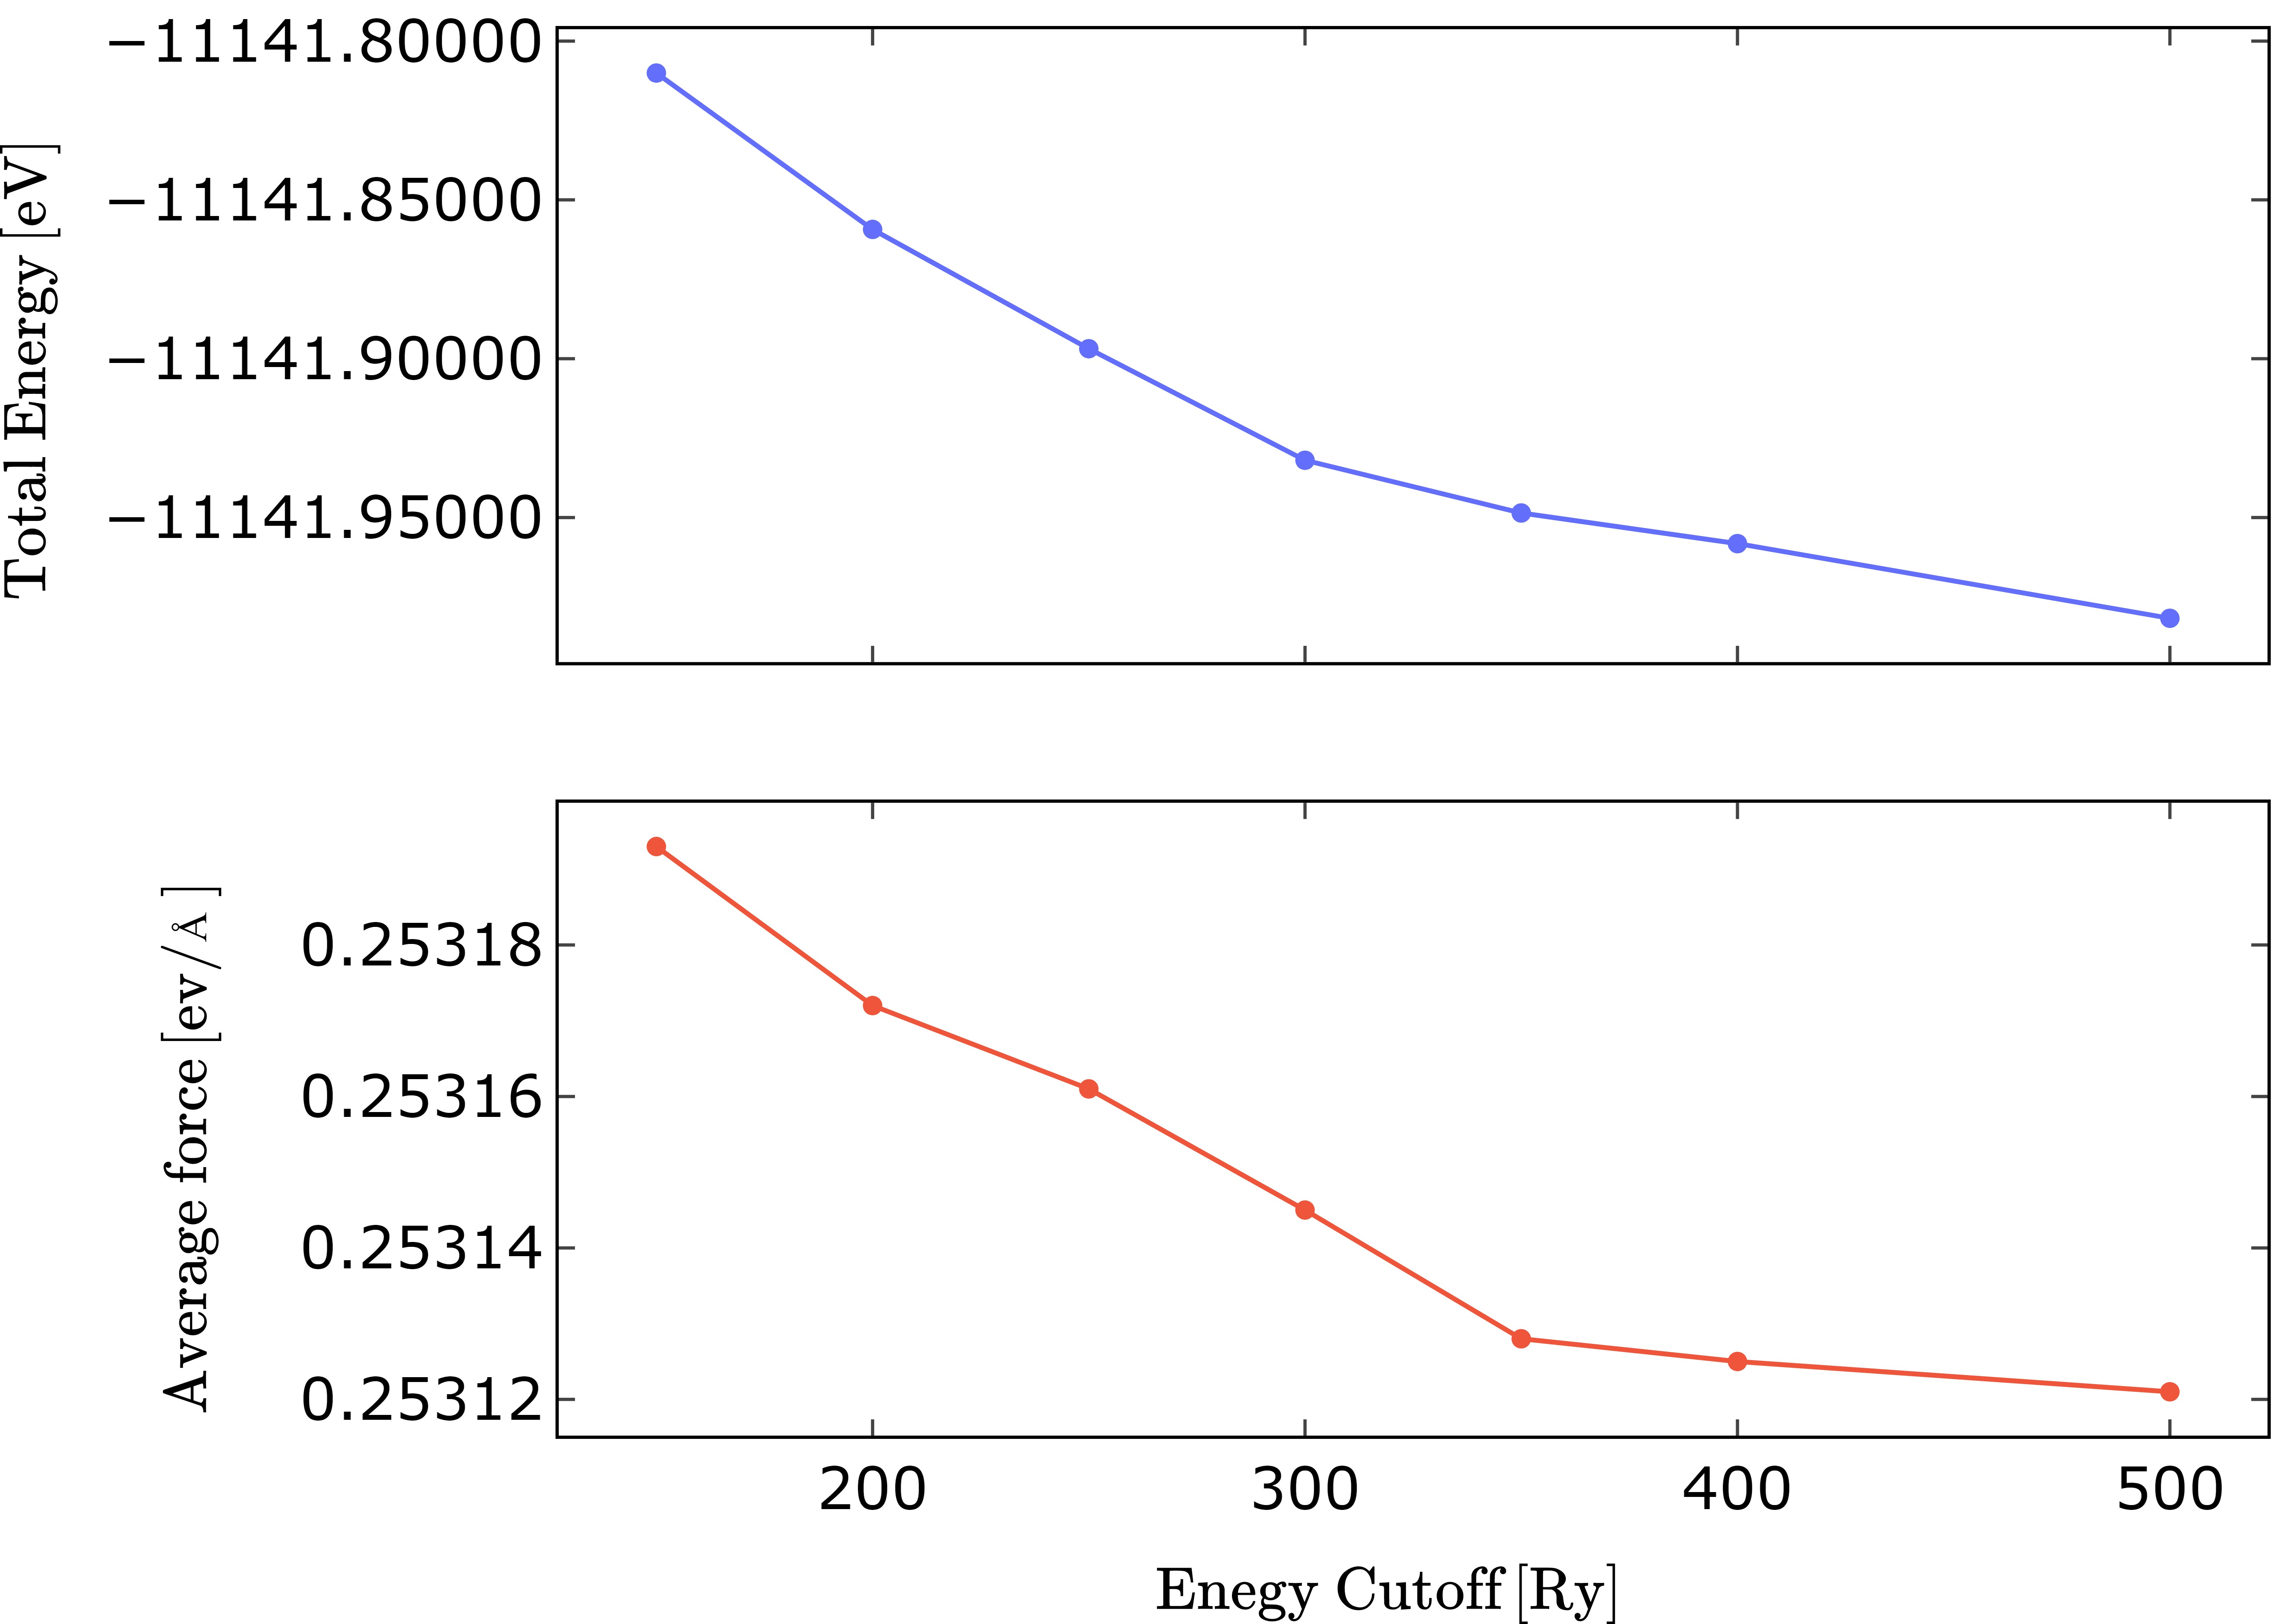
\includegraphics[width=.8\textwidth]{
      asset/cutoff_convergence.jpg
    }
  \end{center}
  \caption{Energy cutoff convergence test for the DFT training data.}
  \label{fig:dft_energy_cutoff_convergence}
\end{figure}

\begin{figure}
  \begin{center}
    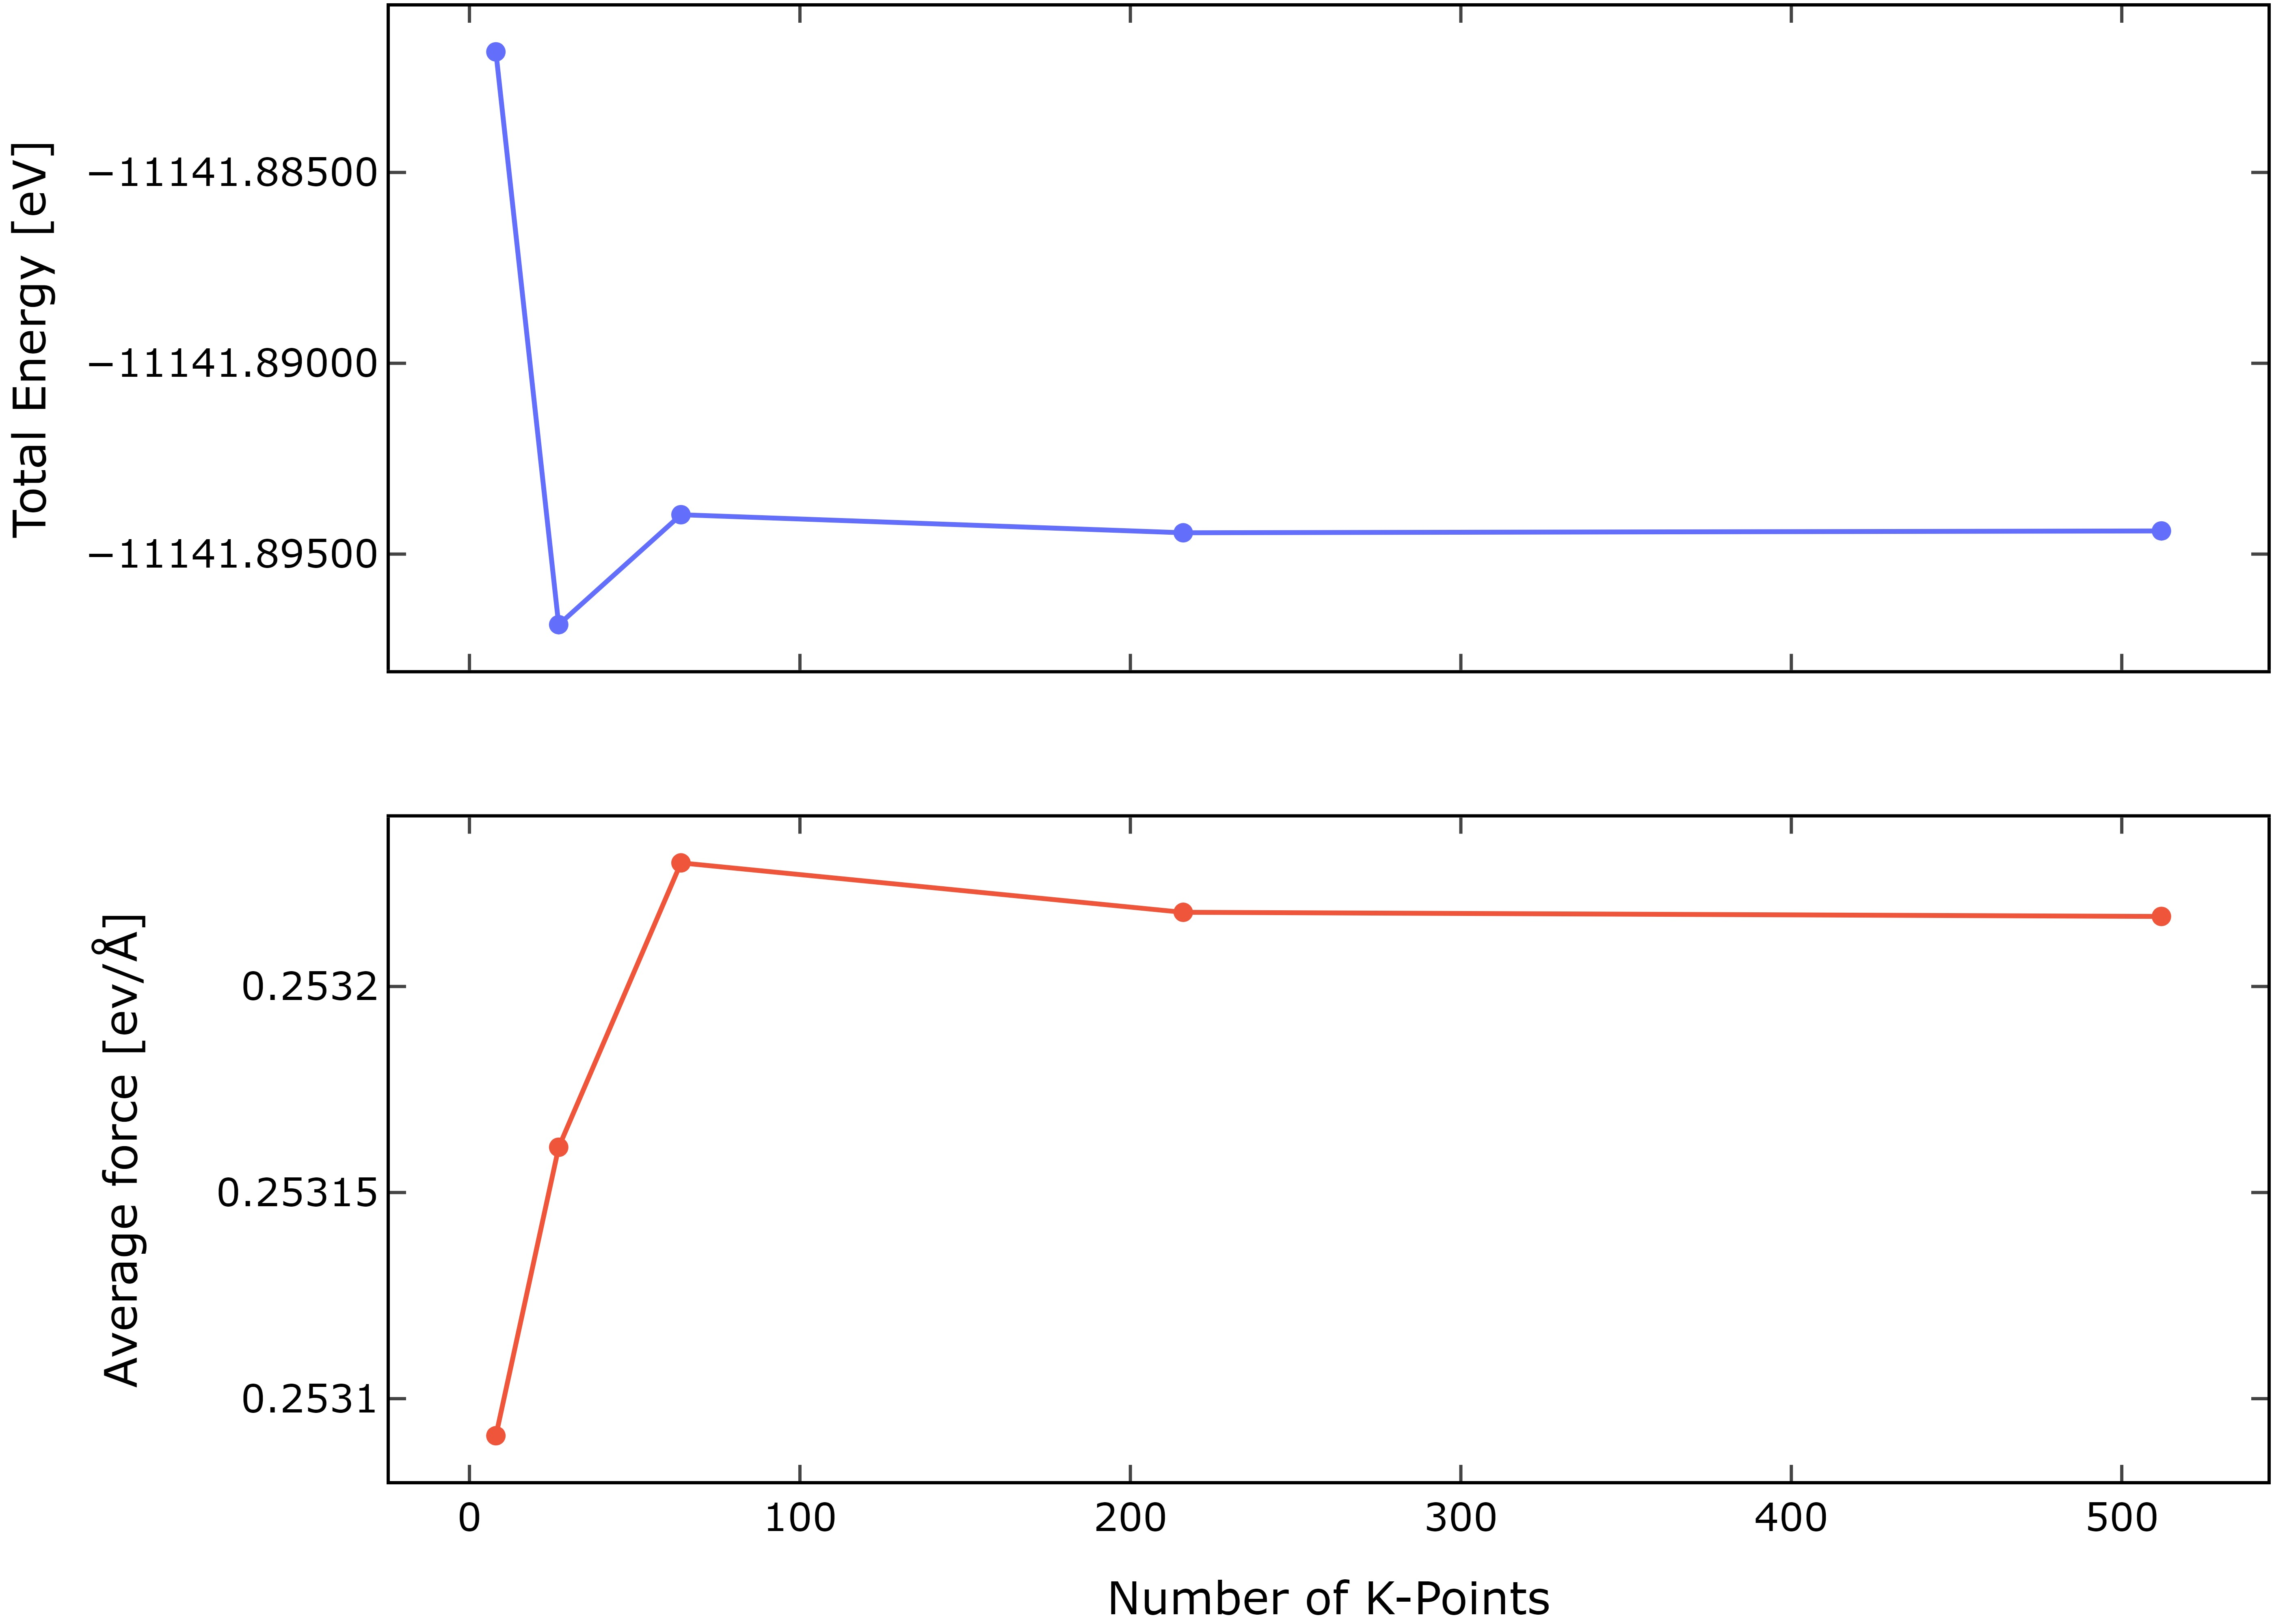
\includegraphics[width=.8\textwidth]{
      asset/kpoint_convergence.jpg
    }
  \end{center}
  \caption{$k$-point convergence test for the DFT training data.}
  \label{fig:dft_kpoint_convergence}
\end{figure}

\section{Training Results}

All models were trained on a dual AMD EPYC 7H12 64-Core processor machine.
Although such specs look impressive, the underlying training algorithms used
by DeepMD-kit seem to not be optimized for CPU training, and the whole process
could probably be greatly accelerated by training on GPUs. DeepMD-kit allows
you to fine-tune the training process by adjusting the runtime parameters
\texttt{OMP\_NUM\_THREADS}, \texttt{TF\_INTRA\_OP\_PARALLELISM\_THREADS},
and \texttt{TF\_INTER\_OP\_PARALLELISM\_\allowbreak{}THREADS}. Despite running
many empirical tests to arrive at the optimal values for these parameters, the
training process did not speed up significantly. The training sessions took
about $12 \, \mathrm{h}$ for the larger models and about $8 \, \mathrm{h}$ for
the smaller models.

A typical descending learning curve was observed for models trained on the
amorphous and combined datasets. When increasing the number of descriptor
neurons from $[5, 10, 20]$ (figure
\ref{fig:amorphous_5,10,20d_20,20,20f_260222622s-learning-curves}) to
$[25, 50, 100]$ (figure
\ref{fig:amorphous_25,50,100d_20,20,20f_260222622s-learning-curves}) we don't
observe significant changes in the learning curves. On the other hand, when
increasing the number of fitting neurons from $[10, 10, 10]$
(figure \ref{fig:amorphous_10,20,40d_10,10,10f_260222622s-learning-curves}) to
$[75, 75, 75]$ (figure
\ref{fig:amorphous_10,20,40d_75,75,75f_260222622s-learning-curves}) we can
observe a very slight divergence of training error and validation error with
increasing training steps. We can see from the error evaluation plot for
descriptor neurons (figure \ref{fig:descriptor_energy_error_evaluation}) that
the energy error slightly decreases with increasing number of descriptor
neurons, although this effect is negligible. This is expected, i.e., a larger
number of parameters in general leads to a better fit. The effect of
increasing energy error with increasing number of fitting neurons can also be
observed in the error evaluation plot for fitting neurons (figure
\ref{fig:fitting_energy_error_evaluation}). Both of these effects are much
more pronounced for the crystalline dataset, where data scarcity is a
significant concern. Although the crystalline system should be the simplest
to model, the shortage of data plays a major role here, which can be observed
in the learning curves and in the energy error evaluation plots. Too large
fitting network architectures for the crystalline set lead to overfitting,
i.e., there are too many free parameters for the available data and, the
training begins to fit the random noise in the data. In fact, this is the
reason why an independent validation dataset is used, as the large divergence
between the training and validation signals overfitting.
The predictions for the crystalline system get outstandingly better for both
the training and validation data when increasing the number of descriptor
neurons from $[5, 10, 20]$ (figure
\ref{fig:crystalline_5,10,20d_20,20,20f_260222622s-learning-curves}) to
$[25, 50, 100]$ (figure
\ref{fig:crystalline_25,50,100d_20,20,20f_260222622s-learning-curves}) for
both validation and training datasets. The higher number of descriptor
neurons allows the model to better capture the underlying structure of the
sillicon system, since this effect is observable for the amorphous and
combined systems as well. While the number of descriptor neurons in the tested
range correlates positively with inference quality, the opposite is true for
the number of fitting neurons. When increasing fitting neurons from
$[10, 10, 10]$
(figure \ref{fig:crystalline_10,20,40d_10,10,10f_260222622s-learning-curves})
to $[75, 75, 75]$
(figure \ref{fig:crystalline_10,20,40d_75,75,75f_260222622s-learning-curves})
we observe that the energy error increases and the dissonance between
training error and validation error broadens. In this case, the model
architecture is too complex and overfits on the small sample of training data.
We can also see the discussed effects in the error evaluation plots for
descriptor neurons and fitting neurons (figures
\ref{fig:descriptor_energy_error_evaluation} and
\ref{fig:fitting_energy_error_evaluation} respectively).

The force errors in all of the learning curves seem to converge relatively
quickly for all of the training sessions. Further training steps don't seem to
significantly improve the prediction quality and may even lead to worse
predictions. This is most likely due to the fact that the forces are very
close to zero for most of the training data, and the models are able to learn
the small deviations from zero very quickly. The increase in force error over
time is caused by the fact that the weights of the objective function are
initially set to prioritize the force error over the energy error and then
gradually shift towards prioritizing energy error over force error, as already
discussed.

\begin{figure}
  \begin{center}
    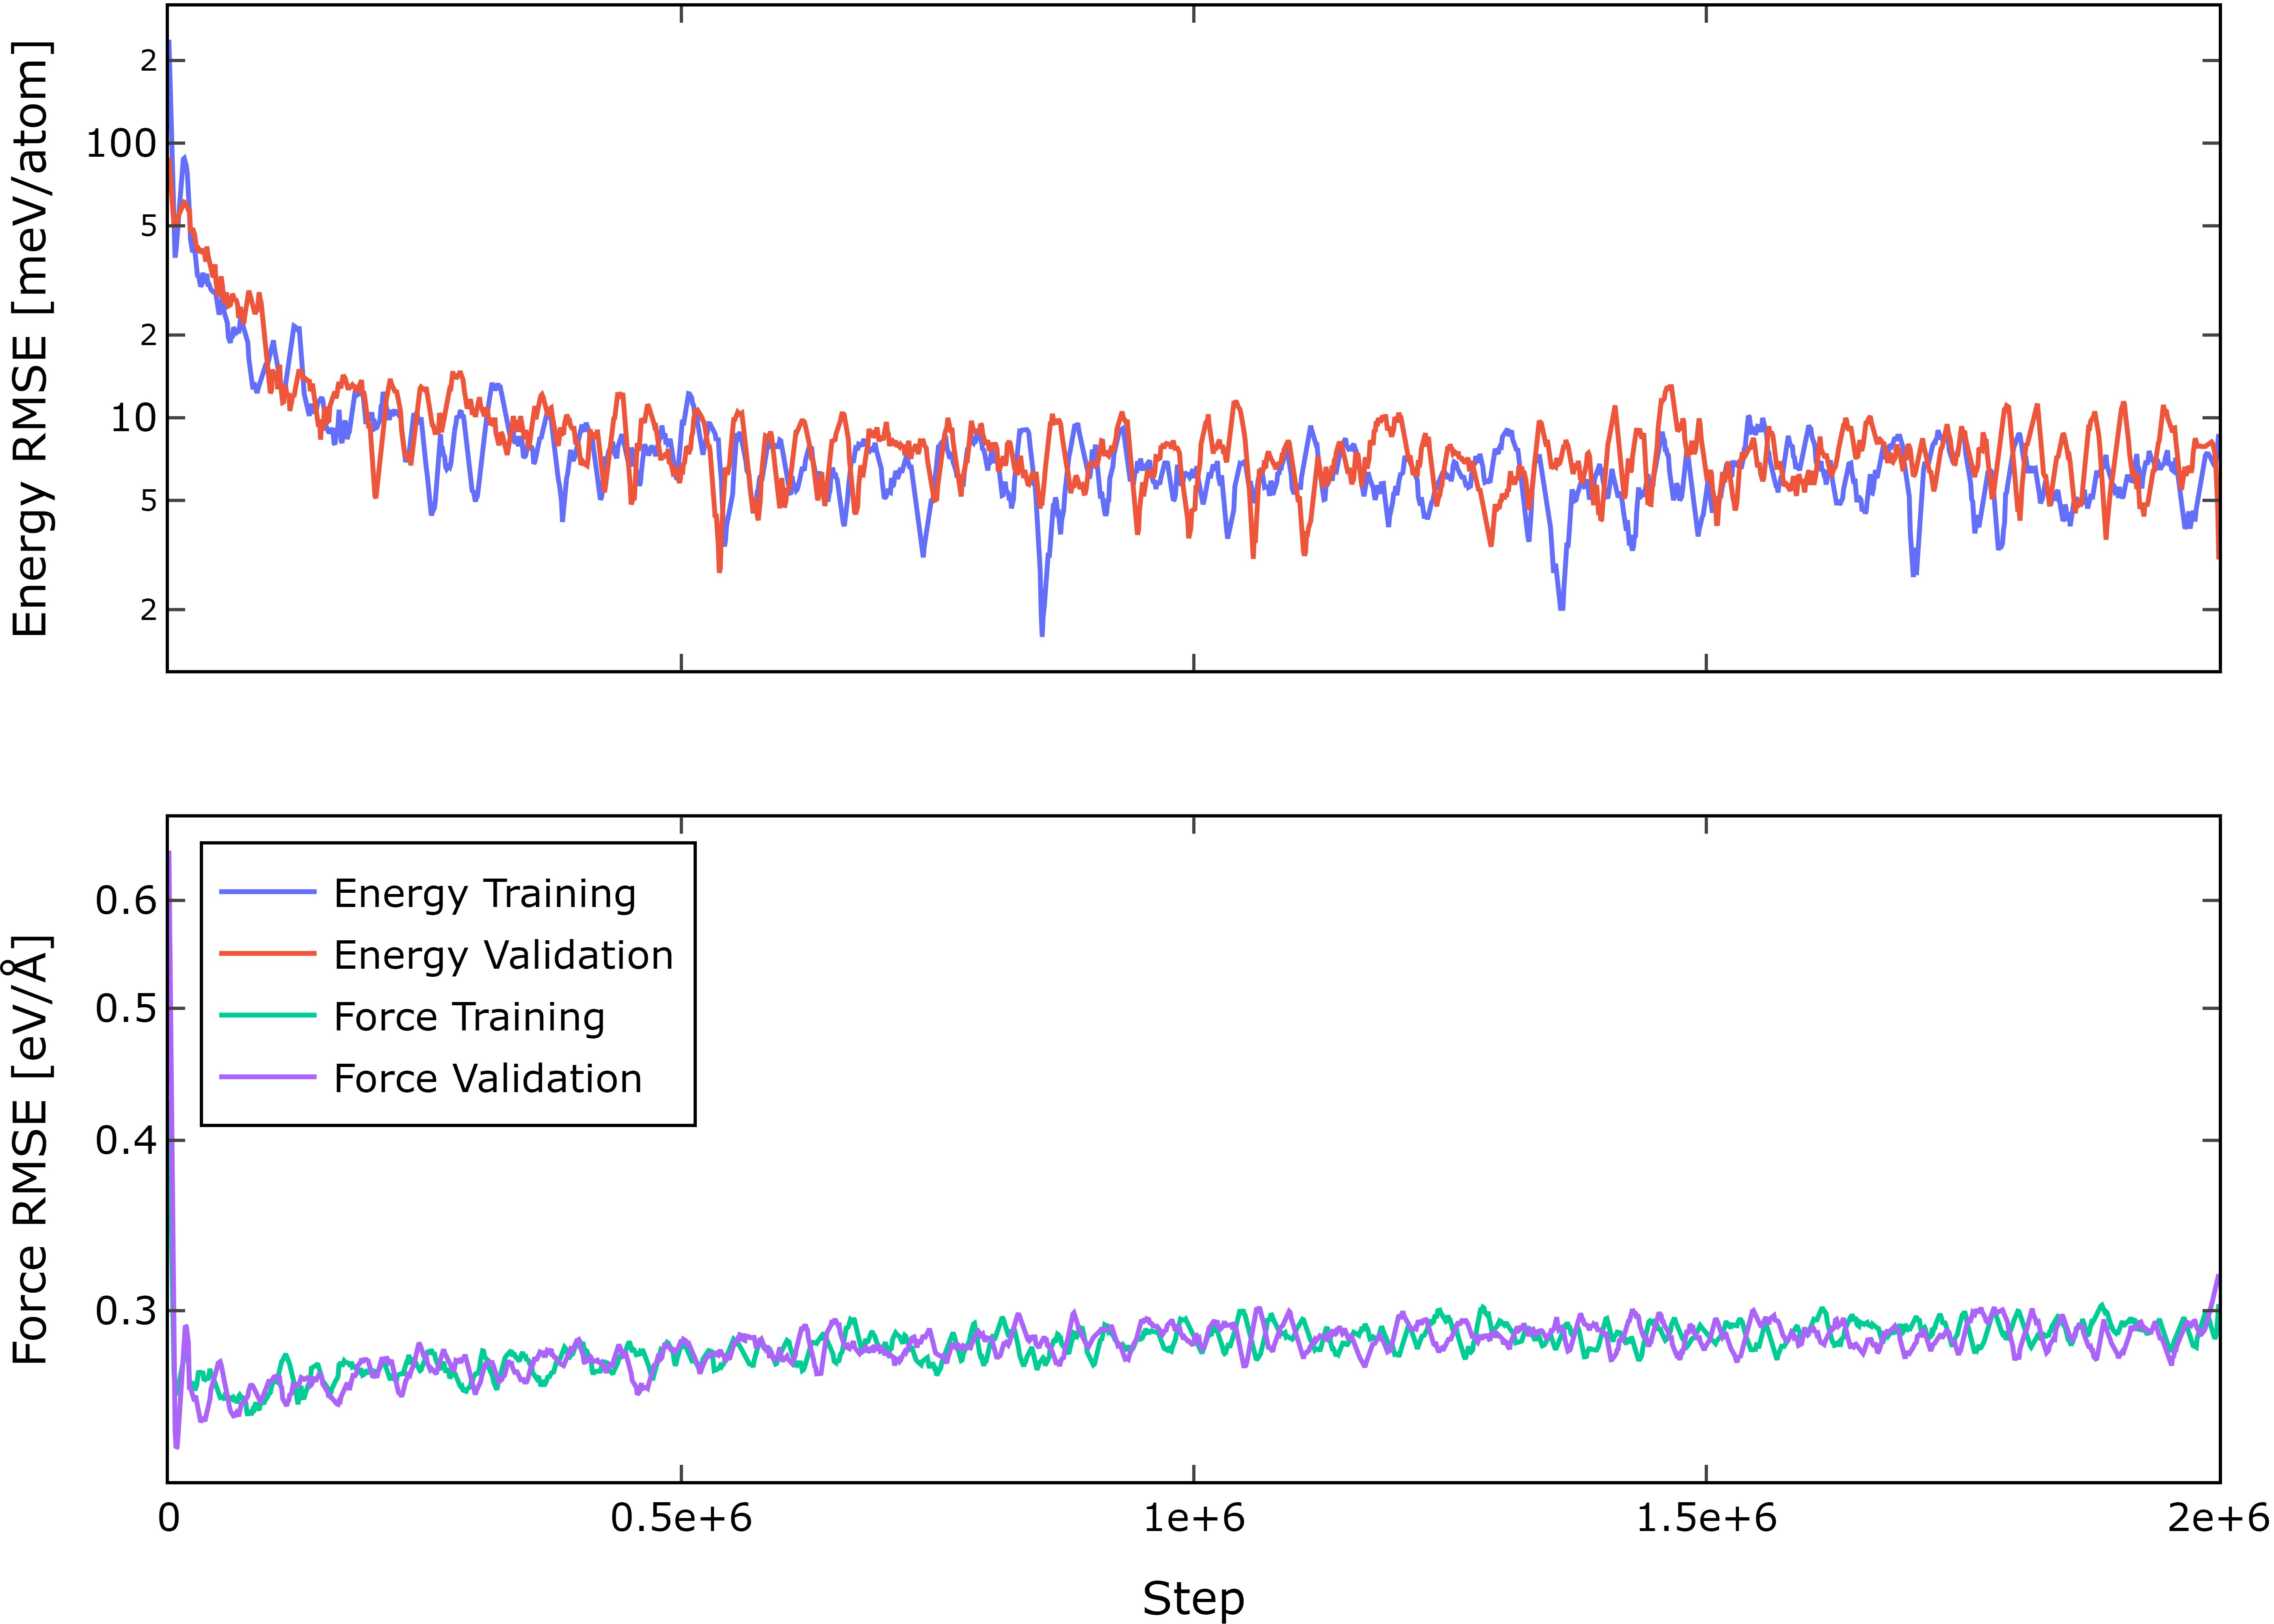
\includegraphics[width=.8\textwidth]{
      asset/amorphous_5,10,20d_20,20,20f_260222622s_energy_force_l_curve.jpg
    }
  \end{center}
  \caption{Learning curves for model \texttt{amorphous\_5,10,20d\_20,20,\allowbreak{}20f\_260222622s}.}
  \label{fig:amorphous_5,10,20d_20,20,20f_260222622s-learning-curves}
\end{figure}

\begin{figure}
  \begin{center}
    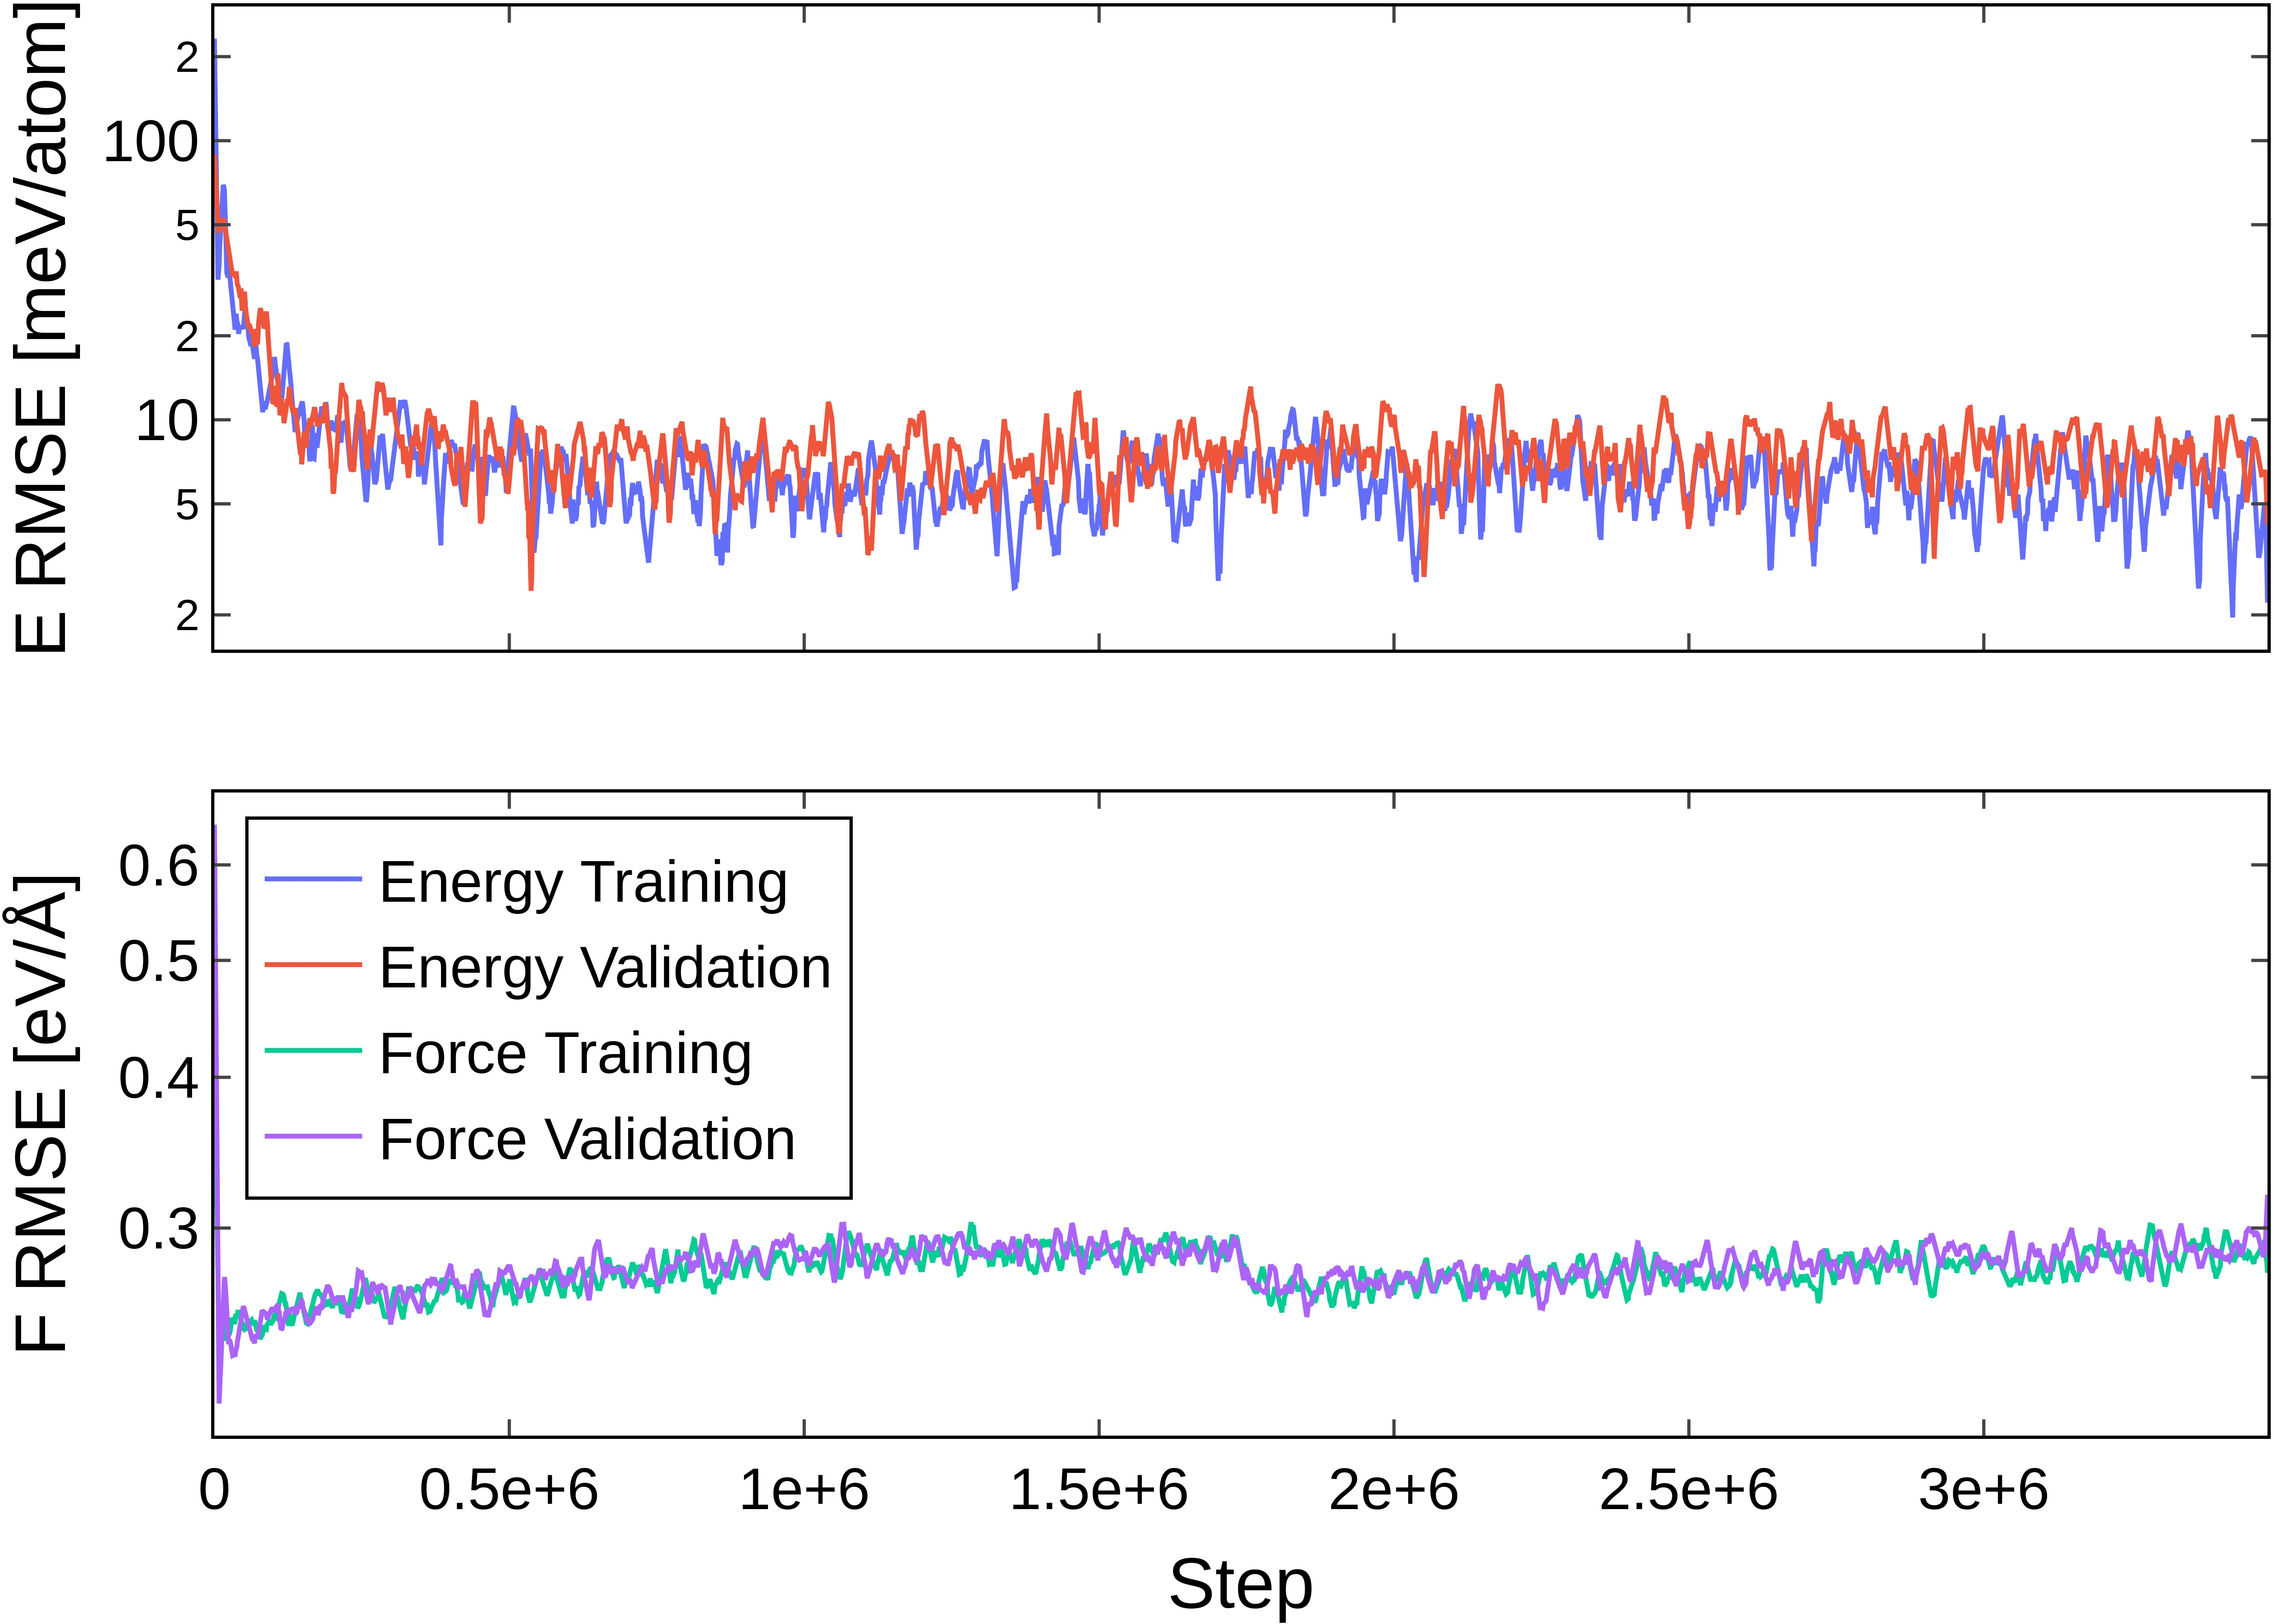
\includegraphics[width=.8\textwidth]{
      asset/amorphous_25,50,100d_20,20,20f_260222622s_energy_force_l_curve.jpg
    }
  \end{center}
  \caption{Learning curves for model \texttt{amorphous\_25,50,100d\_20,20,\allowbreak{}20f\_260222622s}.}
  \label{fig:amorphous_25,50,100d_20,20,20f_260222622s-learning-curves}
\end{figure}


\begin{figure}
  \begin{center}
    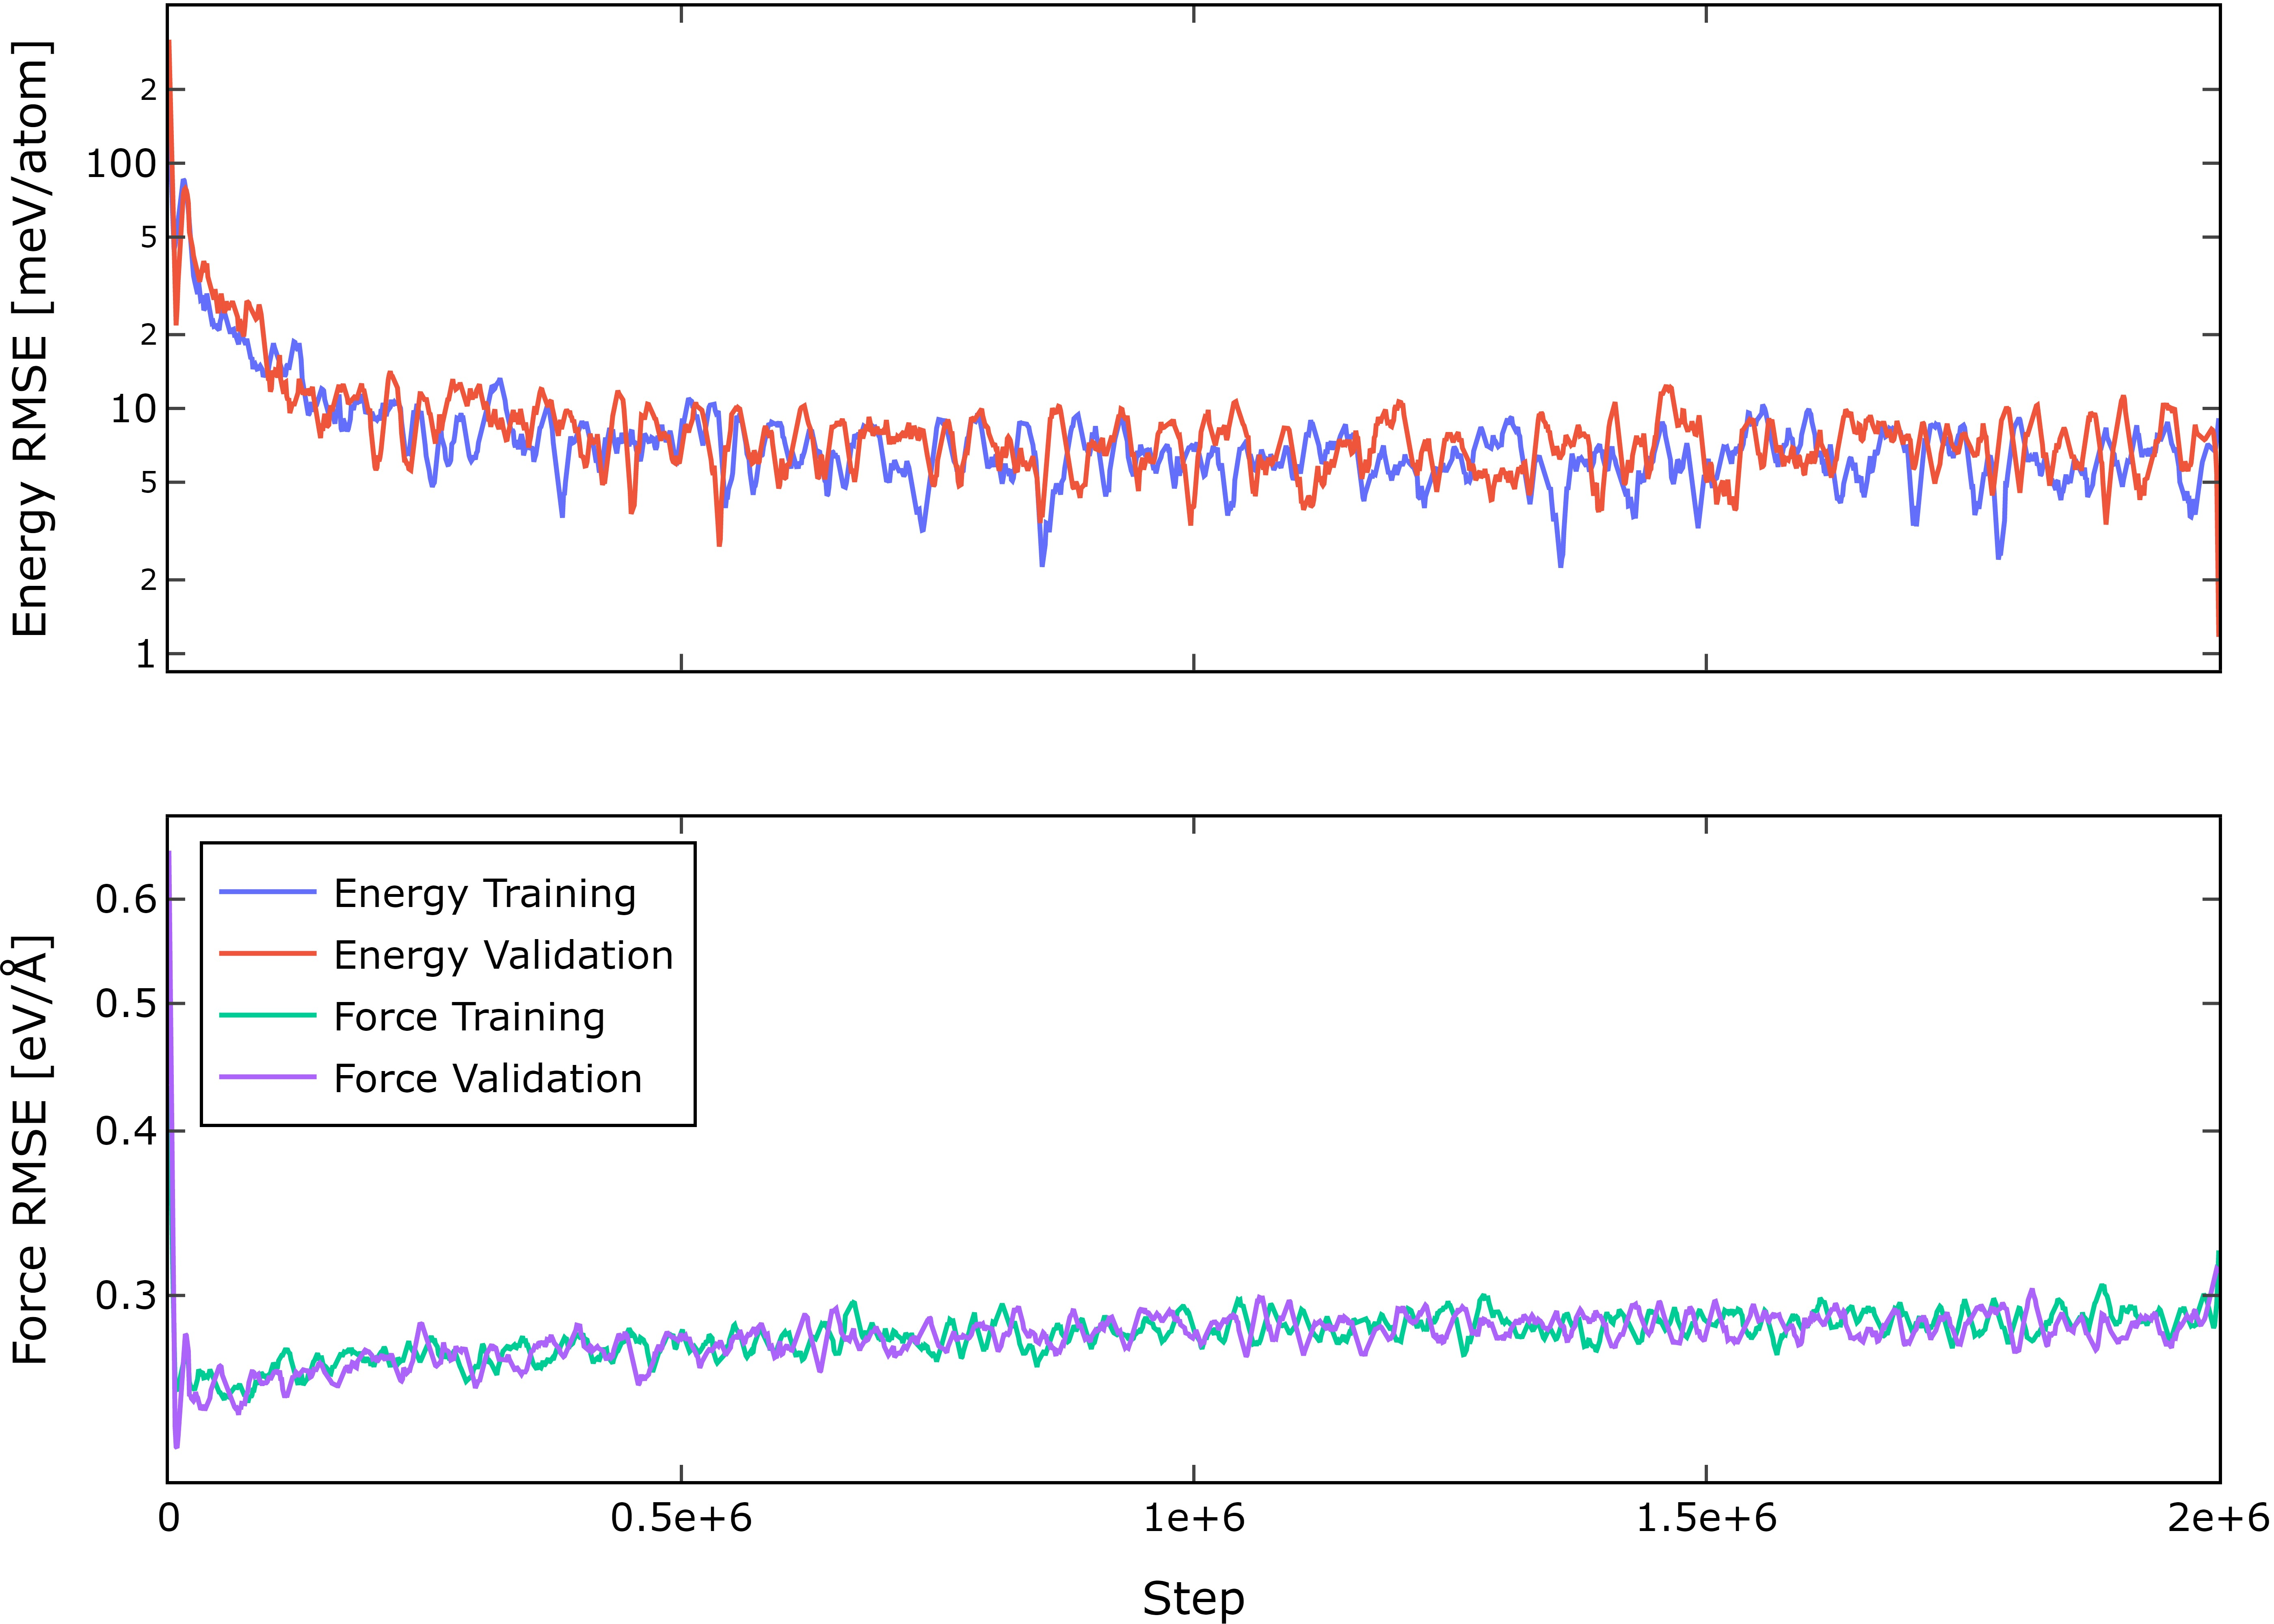
\includegraphics[width=.8\textwidth]{
      asset/amorphous_10,20,40d_10,10,10f_260222622s_energy_force_l_curve.jpg
    }
  \end{center}
  \caption{Learning curves for model \texttt{amorphous\_10,20,40d\_10,10,\allowbreak{}10f\_260222622s}.}
  \label{fig:amorphous_10,20,40d_10,10,10f_260222622s-learning-curves}
\end{figure}

\begin{figure}
  \begin{center}
    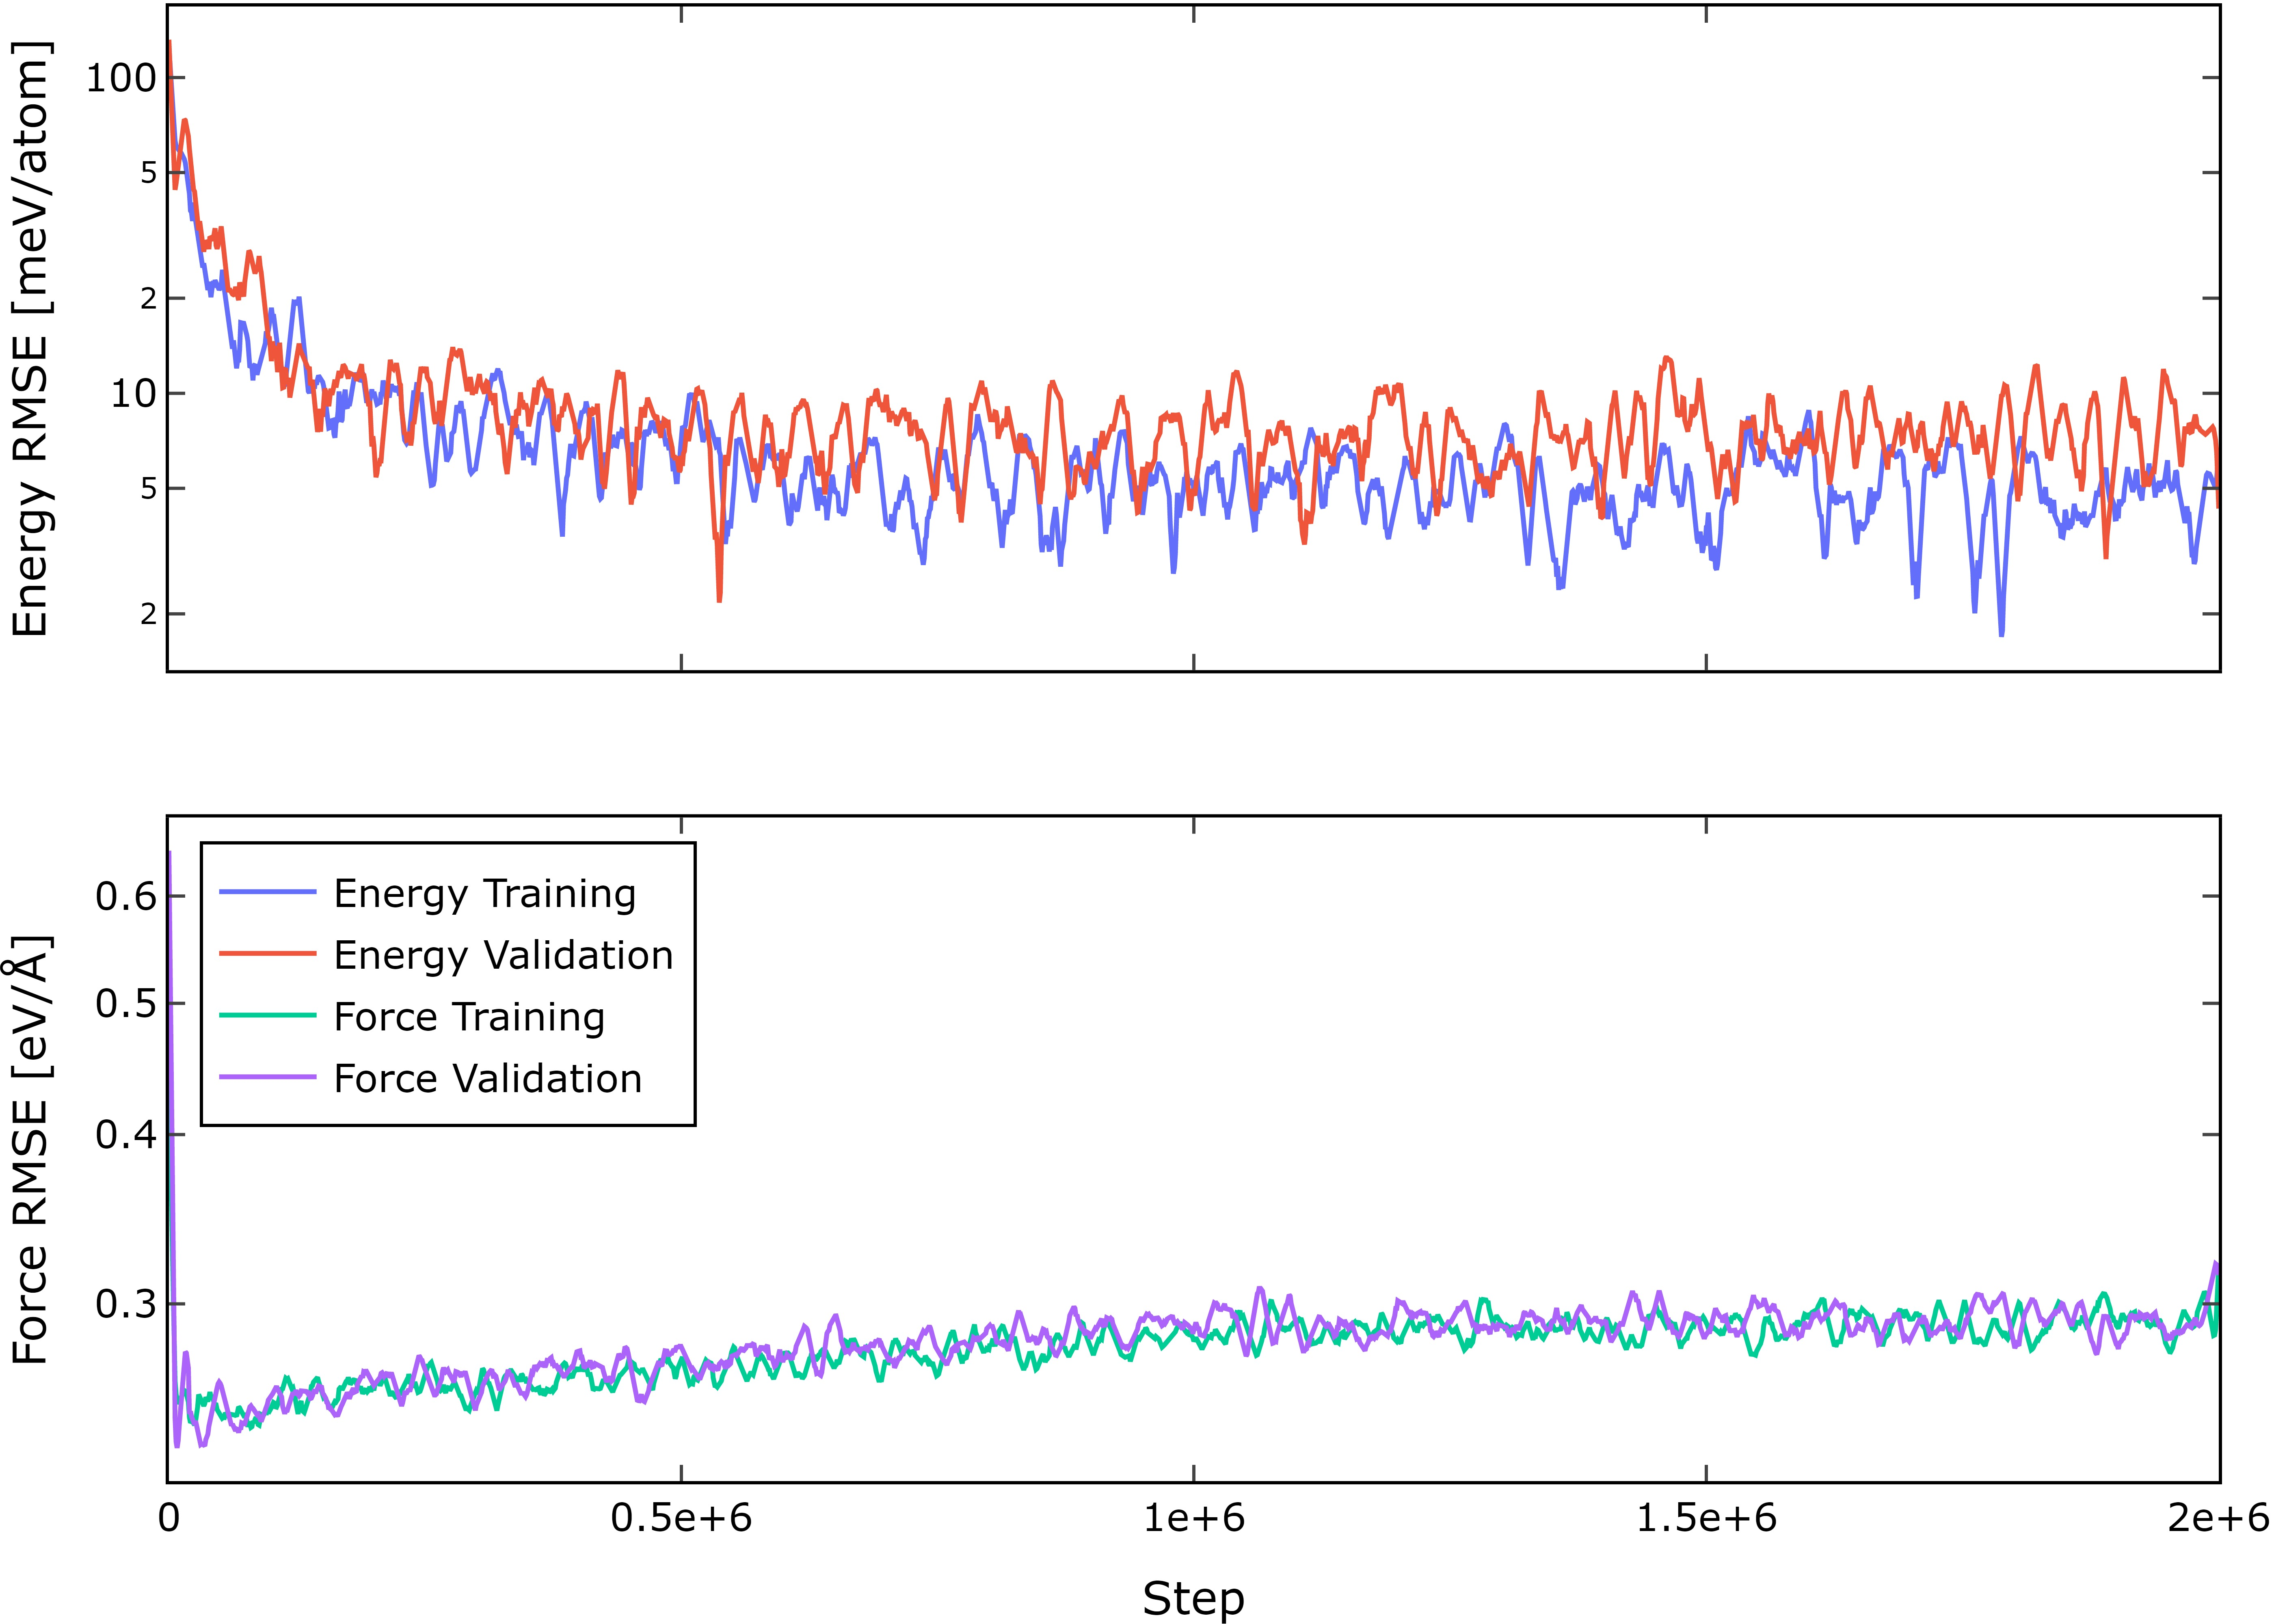
\includegraphics[width=.8\textwidth]{
      asset/amorphous_10,20,40d_75,75,75f_260222622s_energy_force_l_curve.jpg
    }
  \end{center}
  \caption{Learning curves for model \texttt{amorphous\_10,20,40d\_75,75,\allowbreak{}75f\_260222622s}.}
  \label{fig:amorphous_10,20,40d_75,75,75f_260222622s-learning-curves}
\end{figure}

\begin{figure}
  \begin{center}
    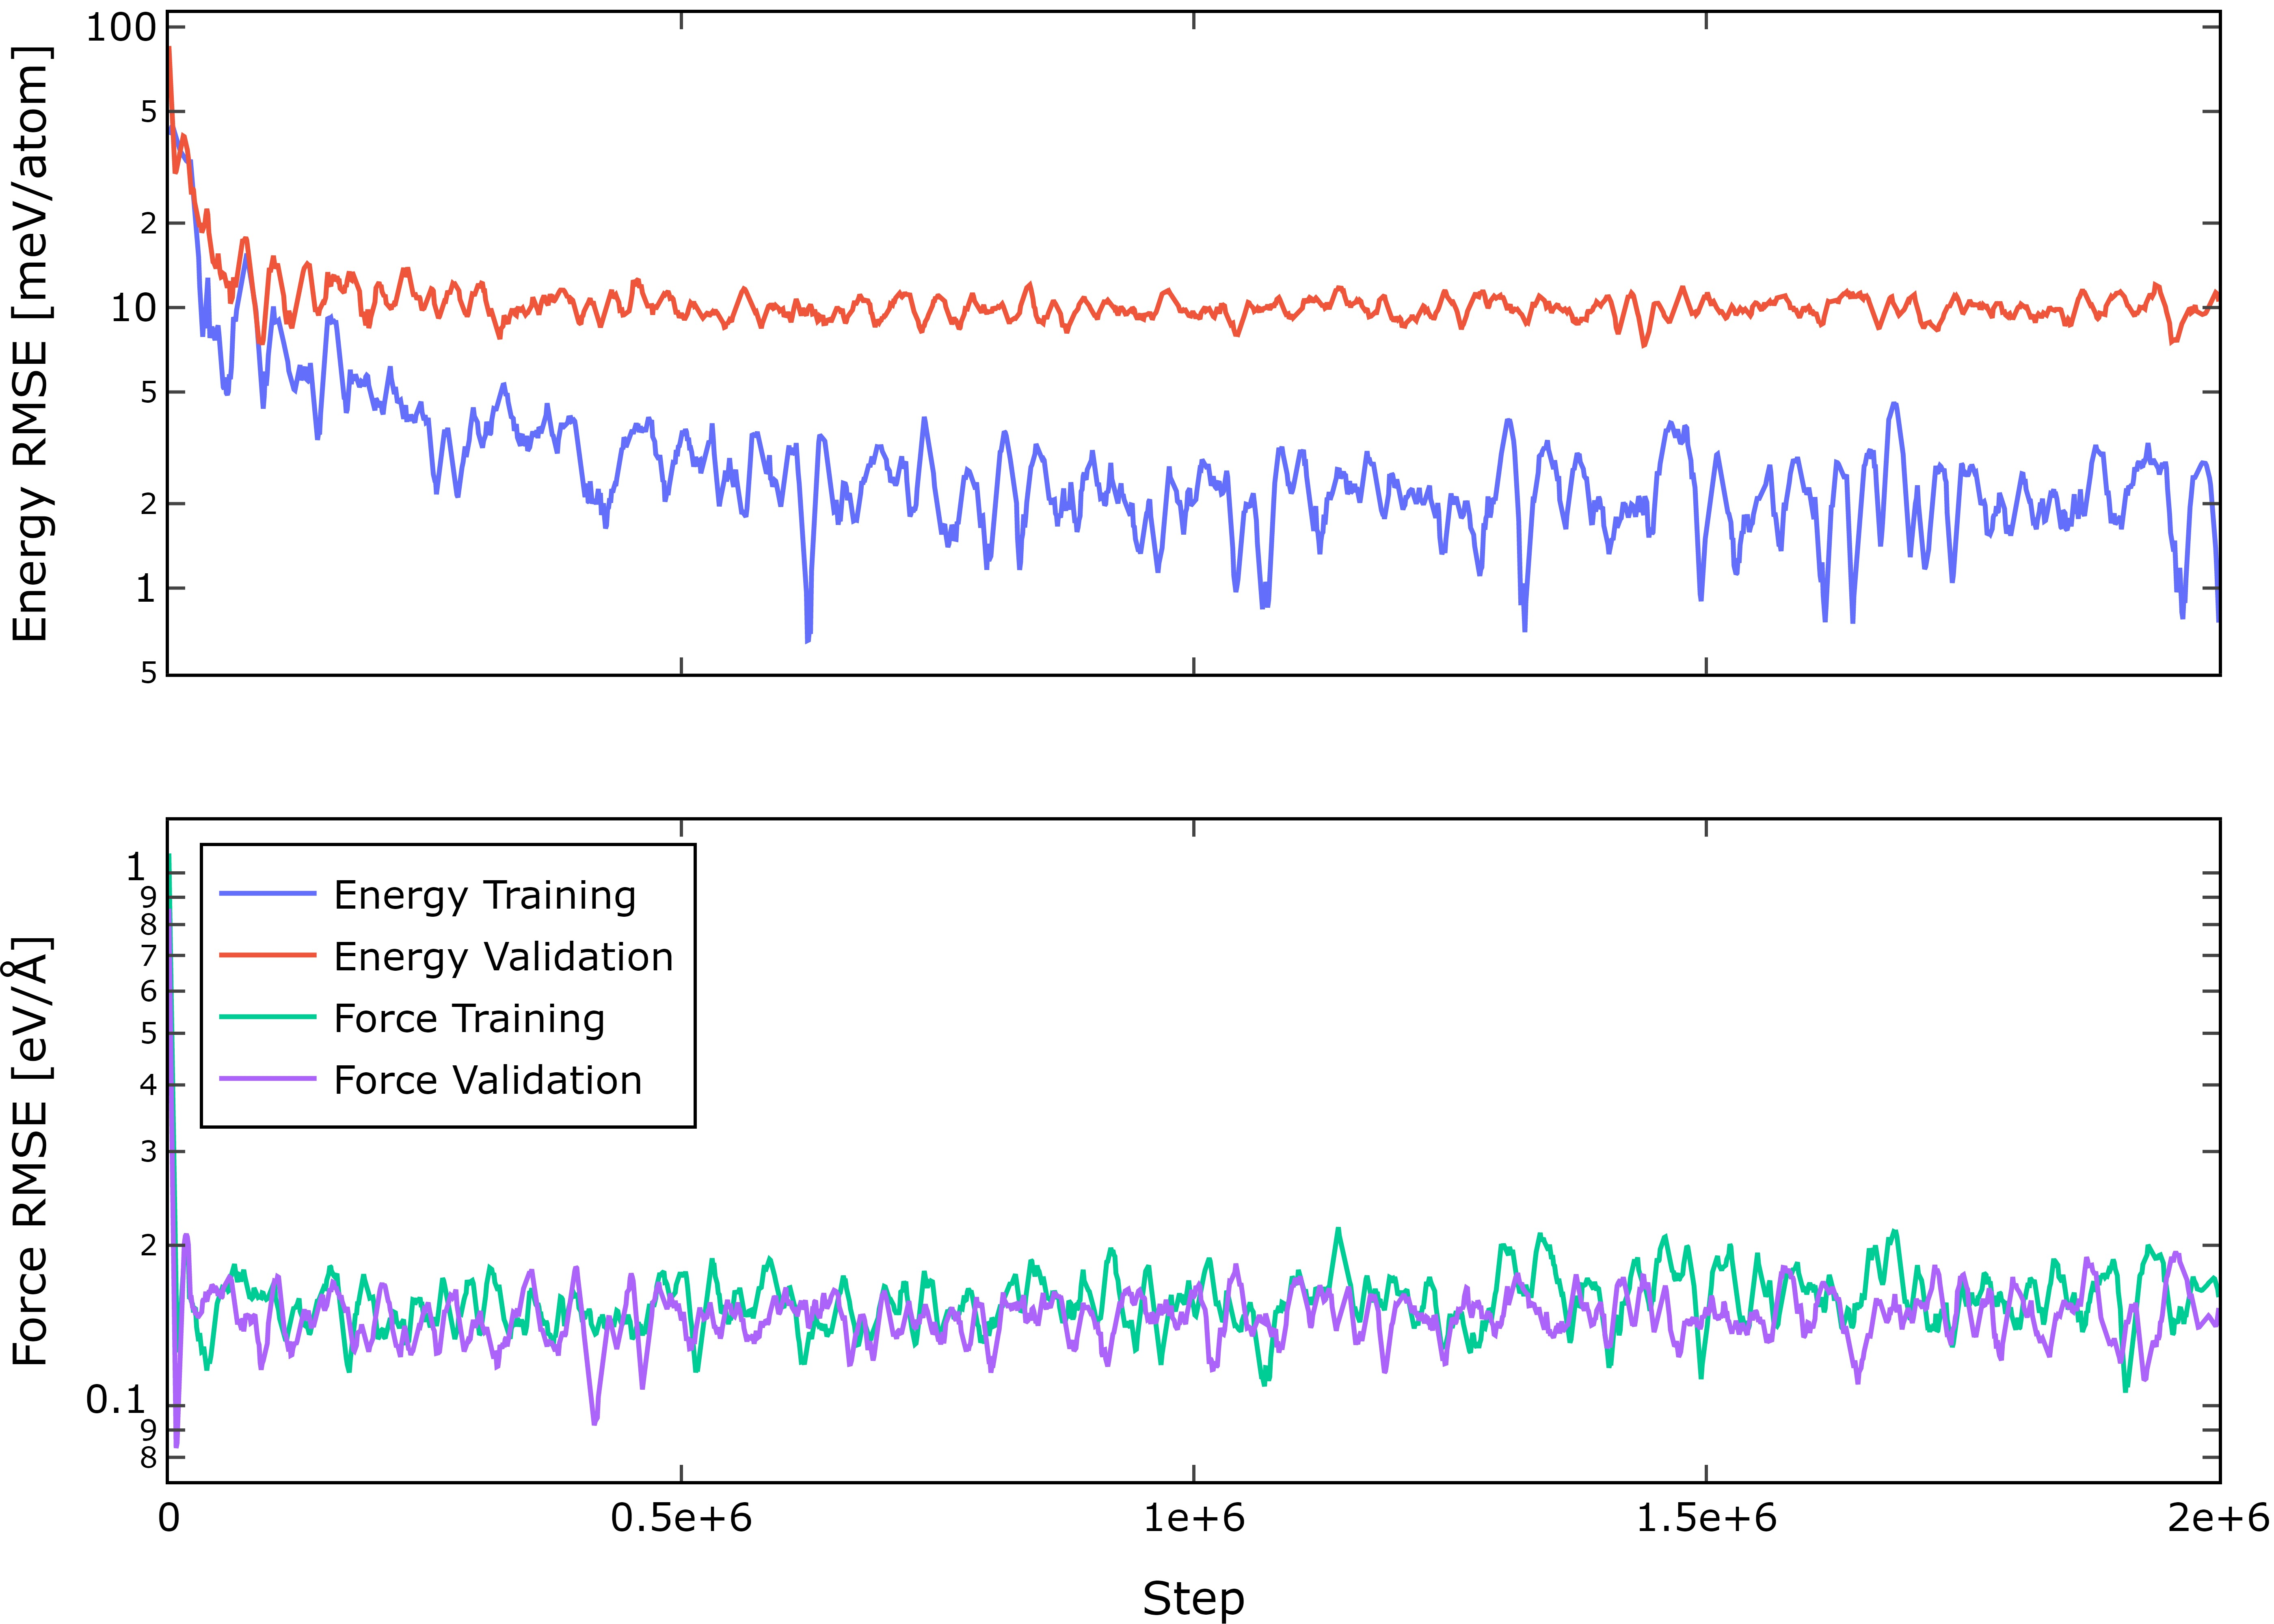
\includegraphics[width=.8\textwidth]{
      asset/crystalline_5,10,20d_20,20,20f_260222622s_energy_force_l_curve.jpg
    }
  \end{center}
  \caption{Learning curves for model \texttt{crystalline\_5,10,20d\_20,20,\allowbreak{}20f\_260222622s}.}
  \label{fig:crystalline_5,10,20d_20,20,20f_260222622s-learning-curves}
\end{figure}

\begin{figure}
  \begin{center}
    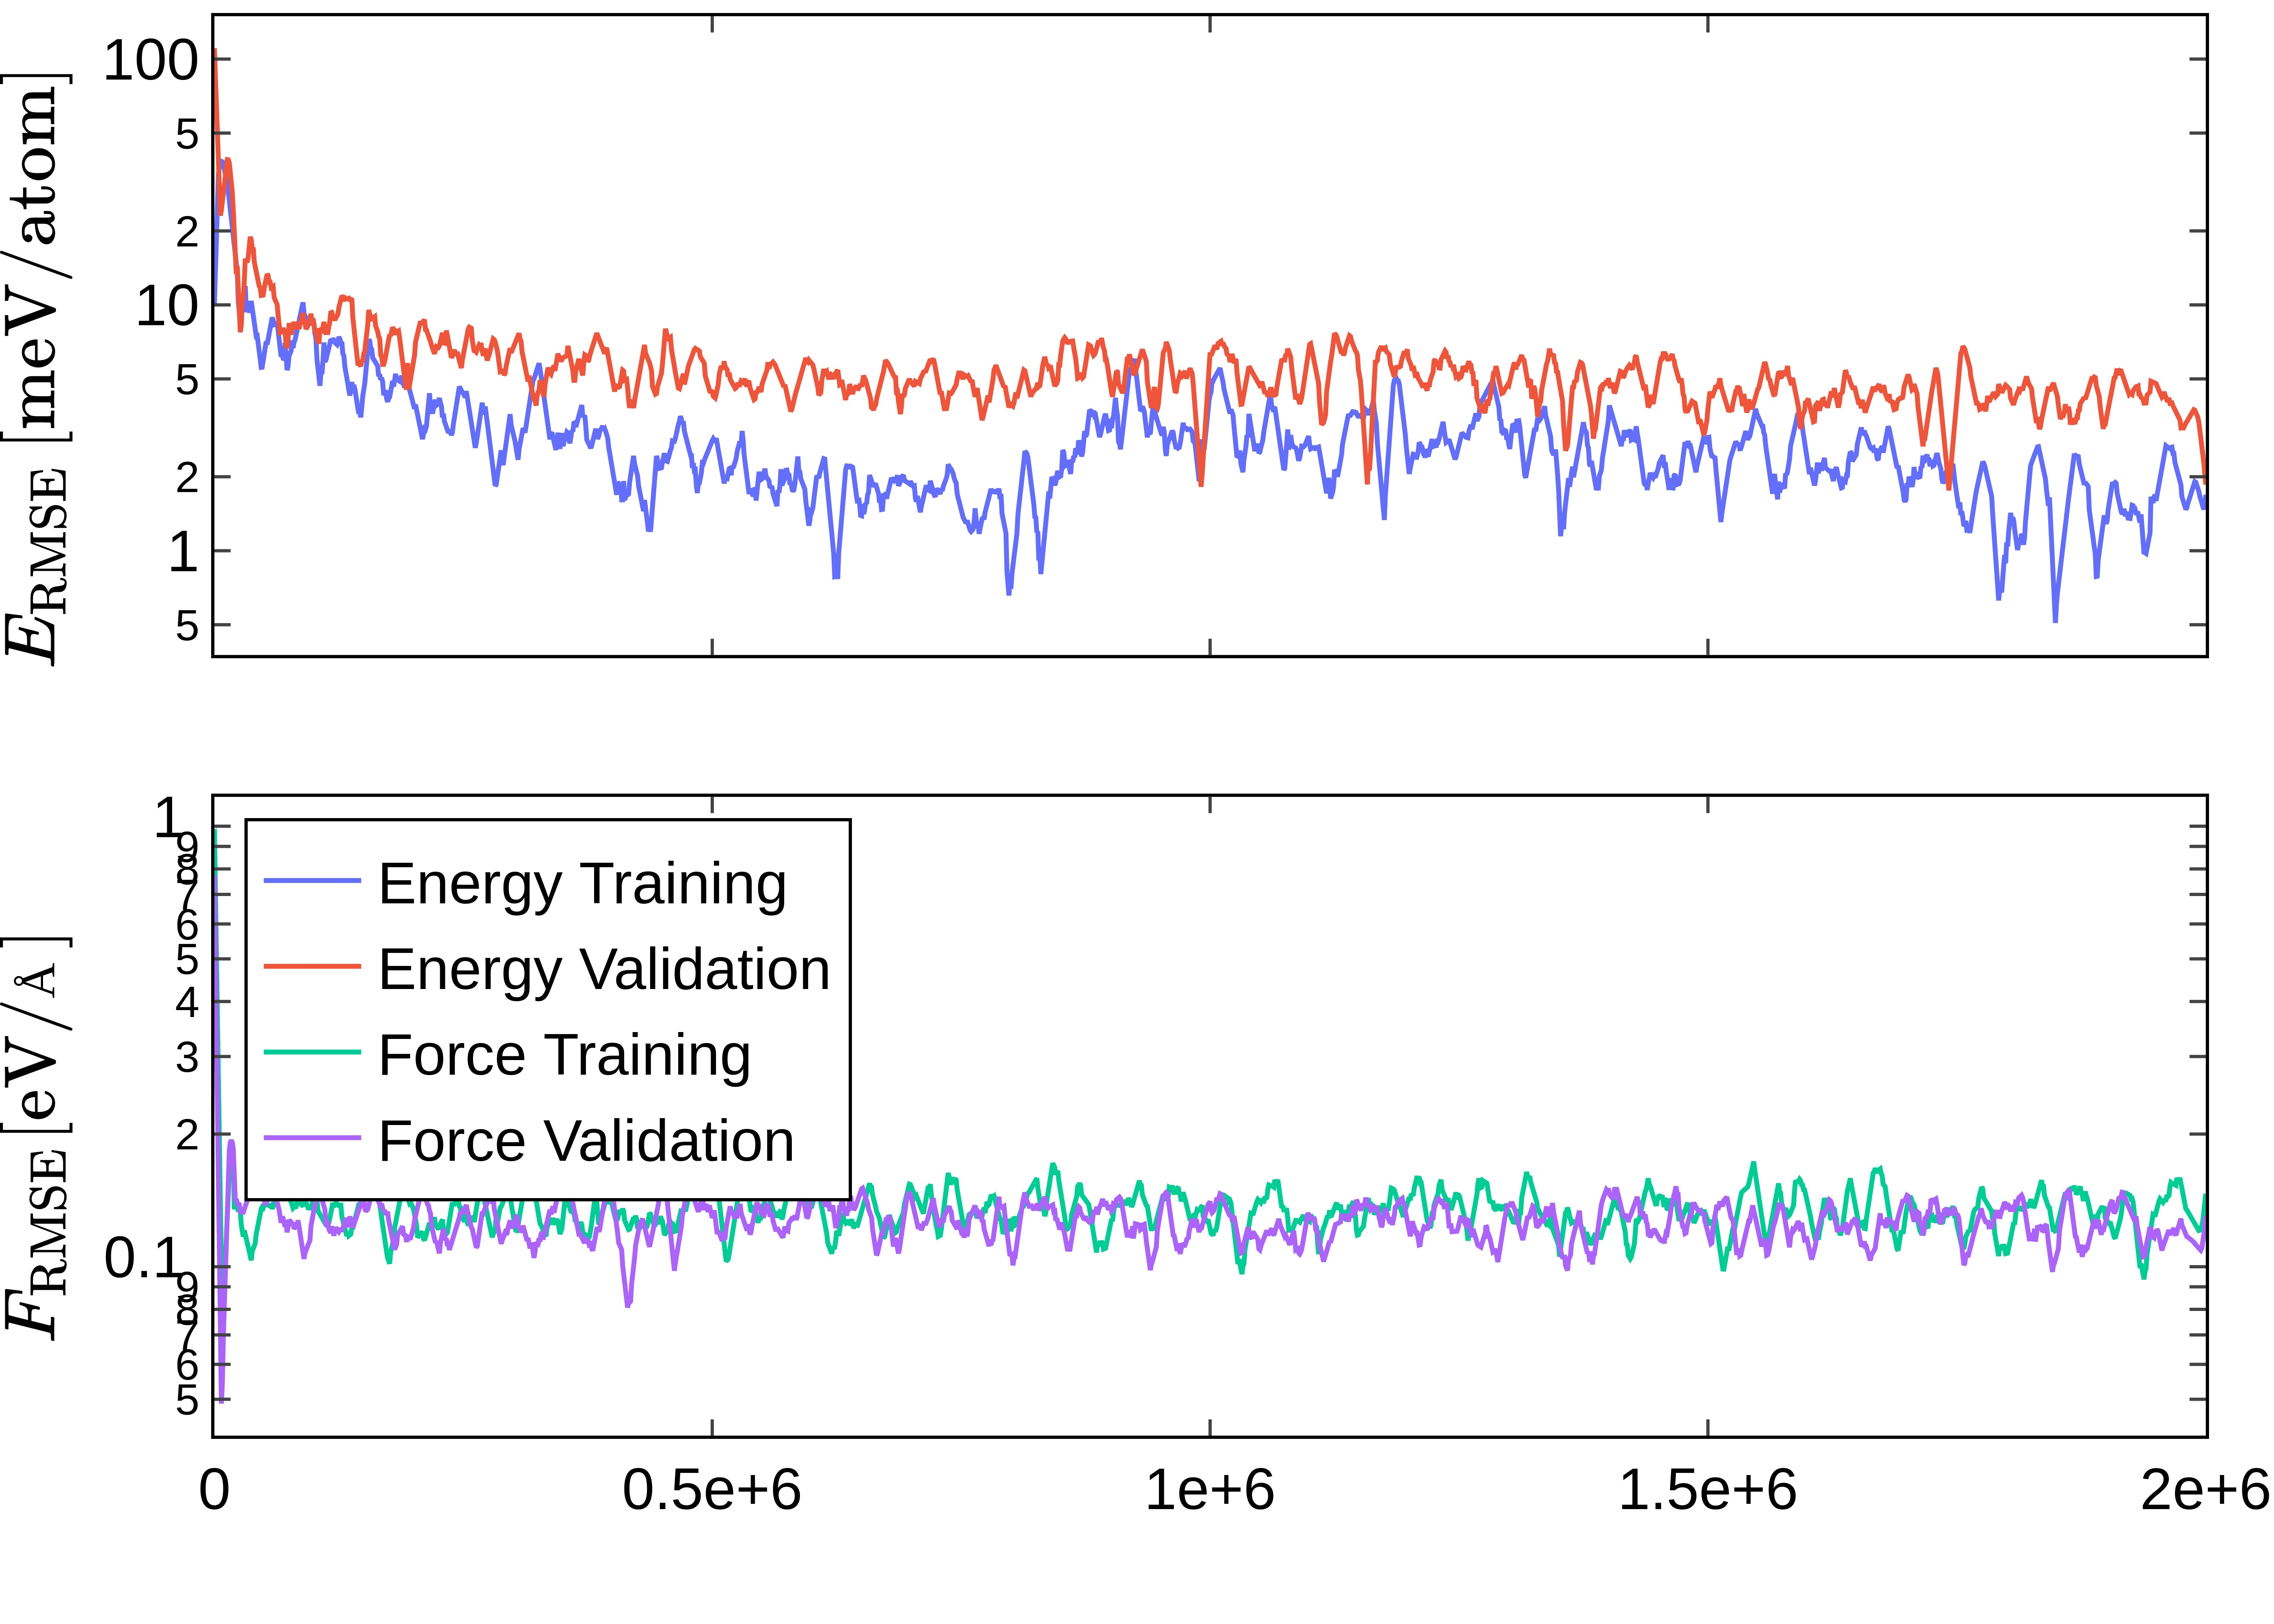
\includegraphics[width=.8\textwidth]{
      asset/crystalline_25,50,100d_20,20,20f_260222622s_energy_force_l_curve.jpg
    }
  \end{center}
  \caption{Learning curves for model \texttt{crystalline\_25,50,100d\_20,20,\allowbreak{}20f\_260222622s}.}
  \label{fig:crystalline_25,50,100d_20,20,20f_260222622s-learning-curves}
\end{figure}

\begin{figure}
  \begin{center}
    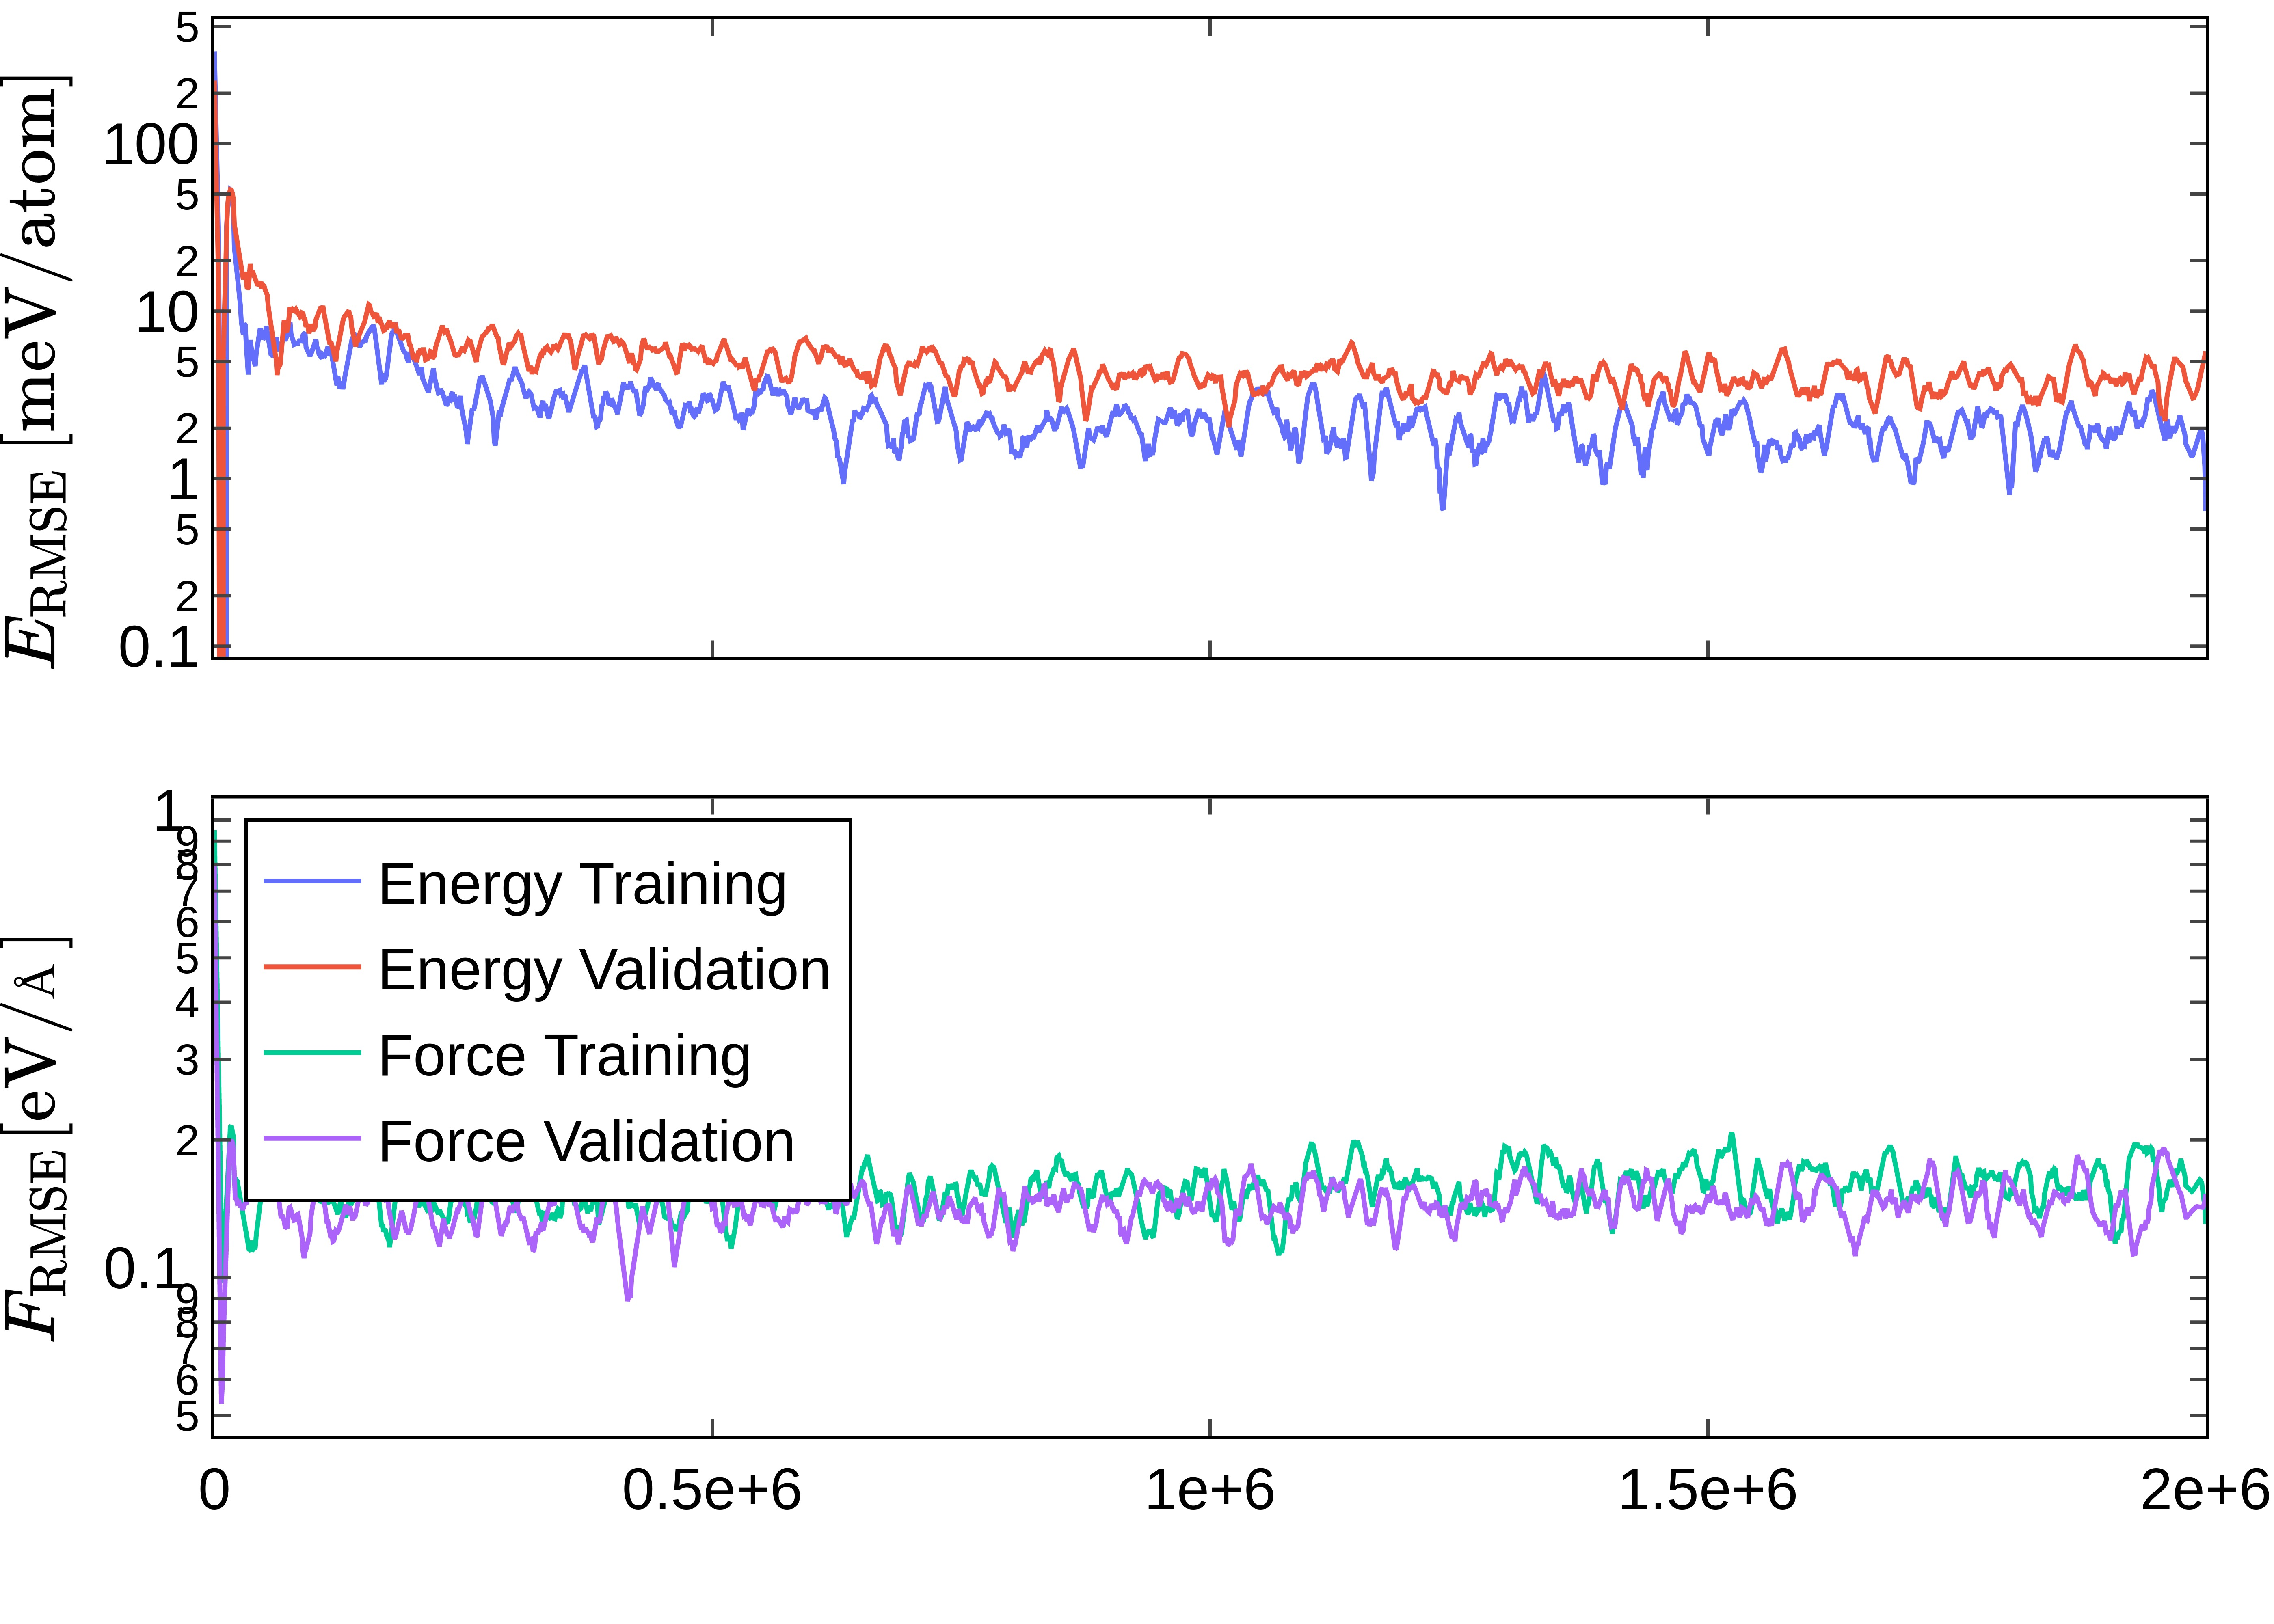
\includegraphics[width=.8\textwidth]{
      asset/crystalline_10,20,40d_10,10,10f_260222622s_energy_force_l_curve.jpg
    }
  \end{center}
  \caption{Learning curves for model \texttt{crystalline\_10,20,40d\_10,10,\allowbreak{}10f\_260222622s}.}
  \label{fig:crystalline_10,20,40d_10,10,10f_260222622s-learning-curves}
\end{figure}

\begin{figure}
  \begin{center}
    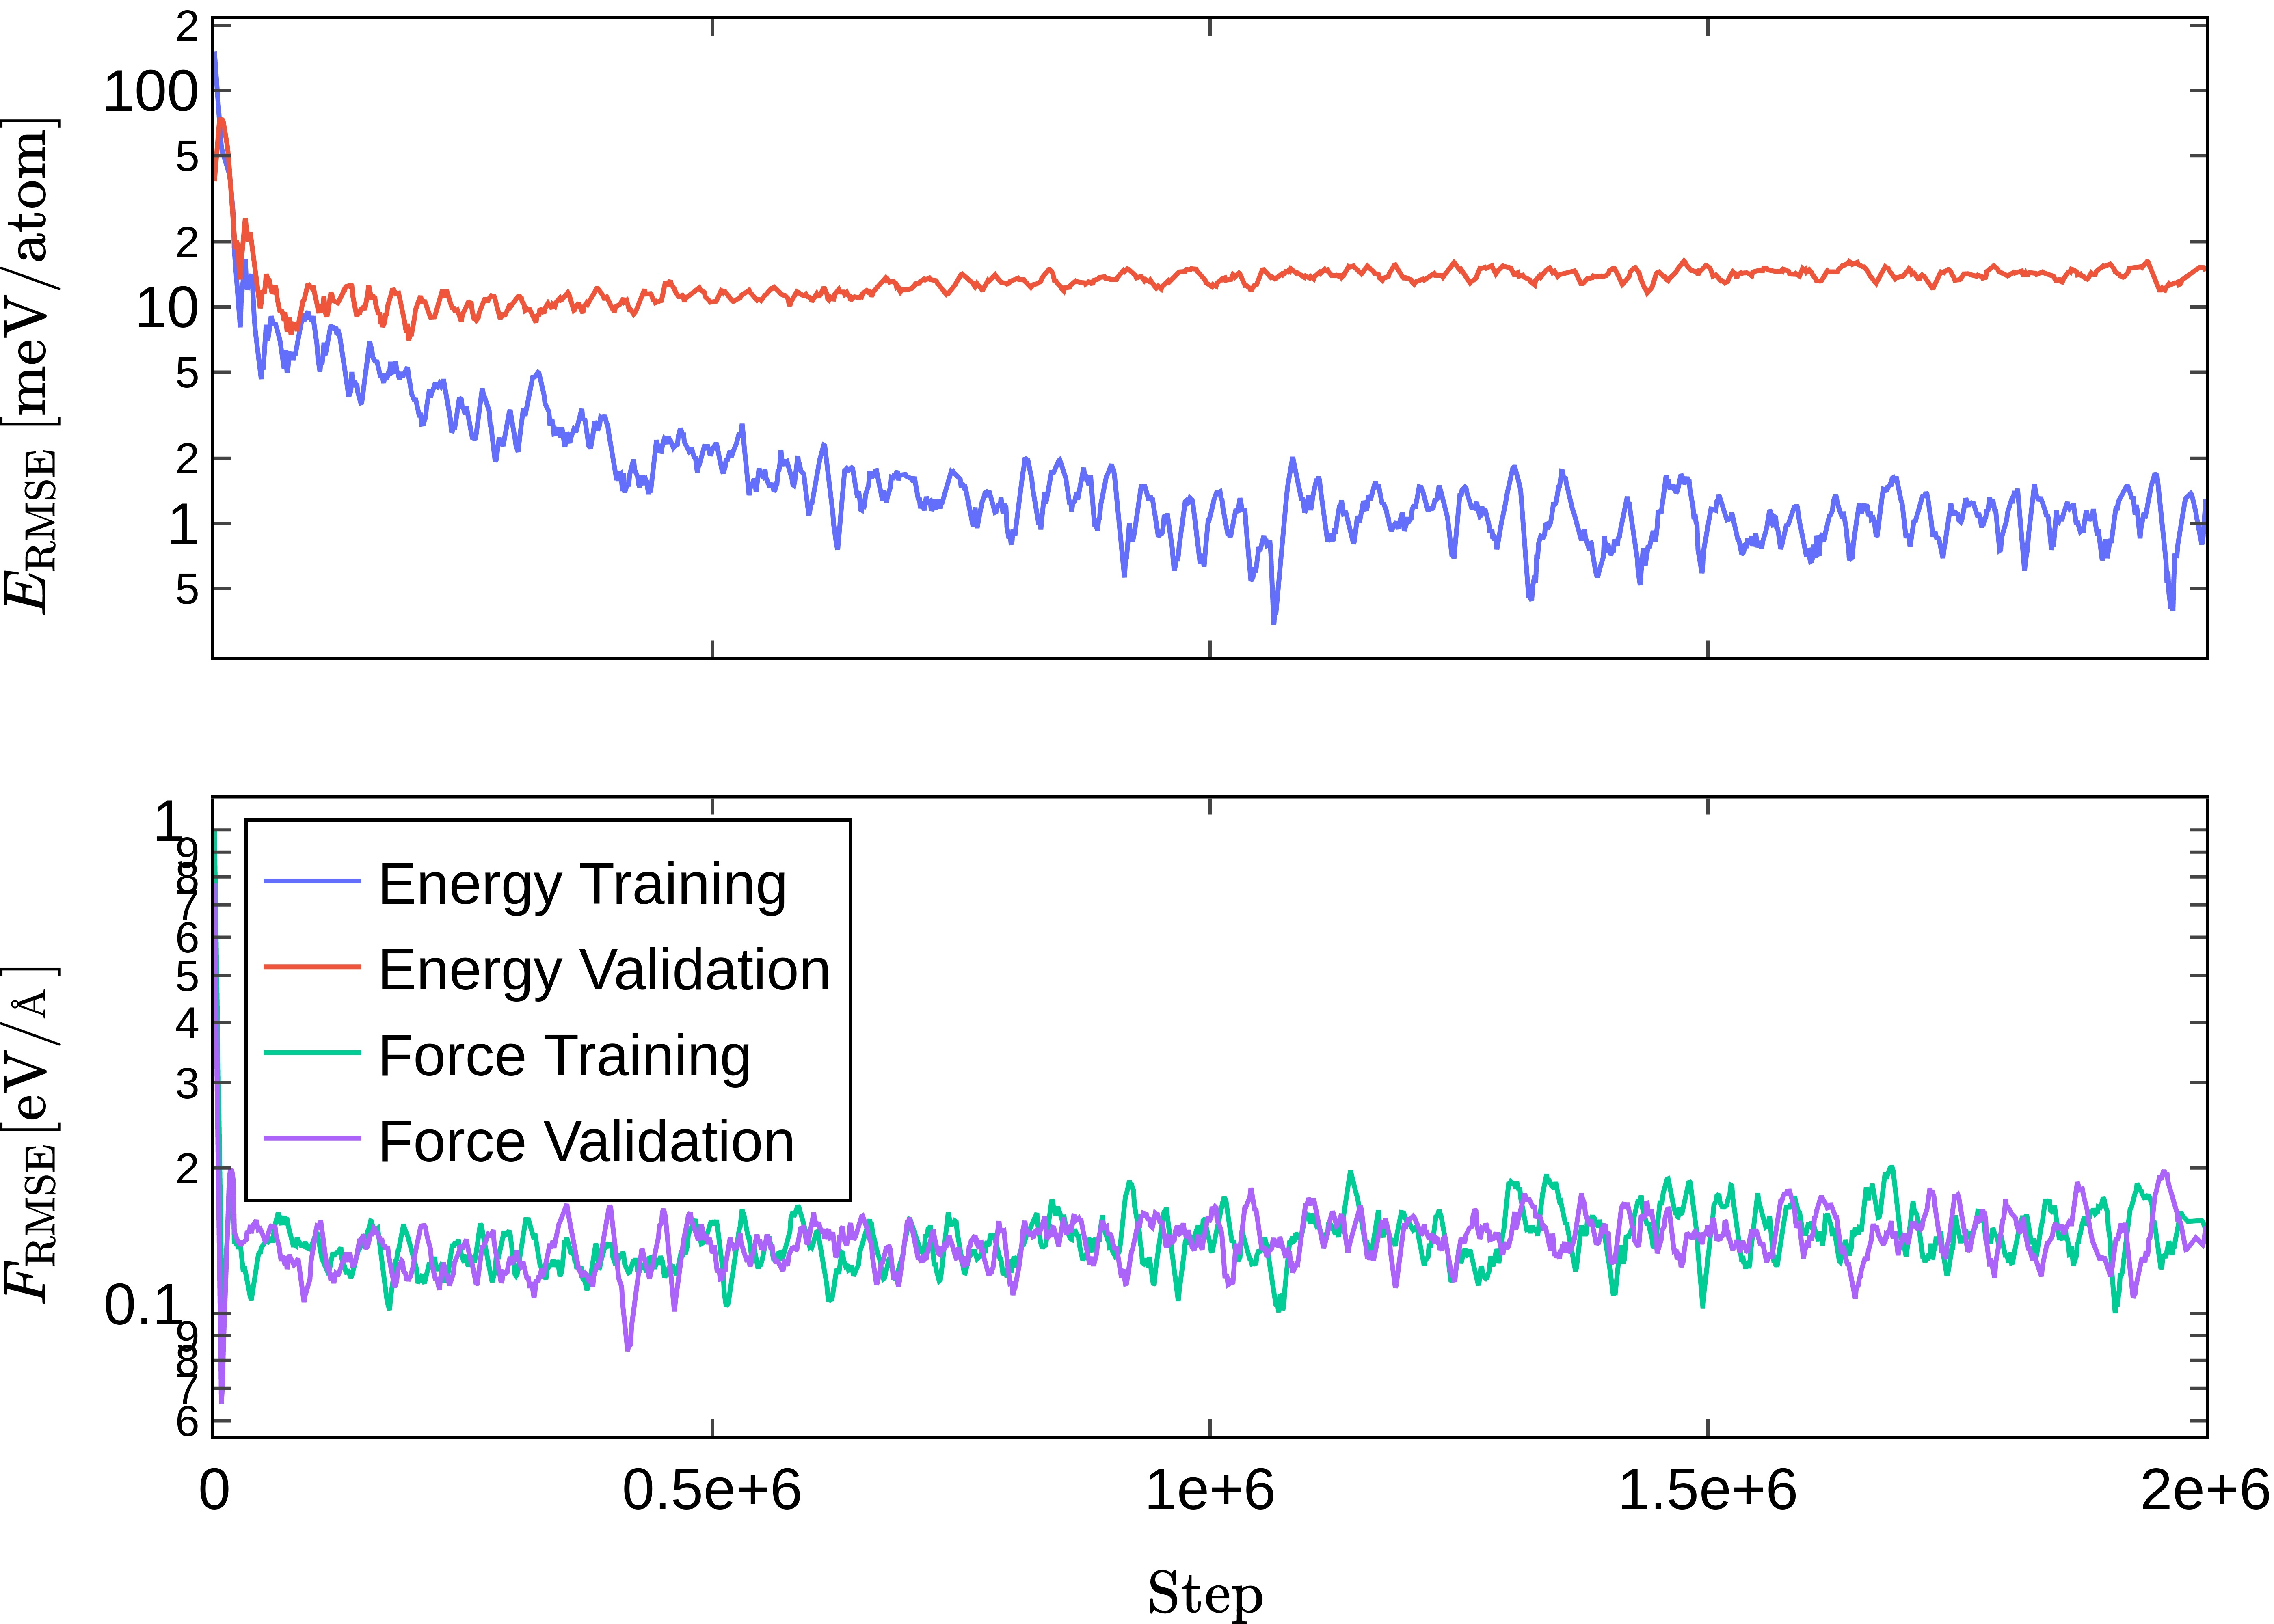
\includegraphics[width=.8\textwidth]{
      asset/crystalline_10,20,40d_75,75,75f_260222622s_energy_force_l_curve.jpg
    }
  \end{center}
  \caption{Learning curves for model \texttt{crystalline\_10,20,40d\_75,75,\allowbreak{}75f\_260222622s}.}
  \label{fig:crystalline_10,20,40d_75,75,75f_260222622s-learning-curves}
\end{figure}

\begin{figure}
  \begin{center}
    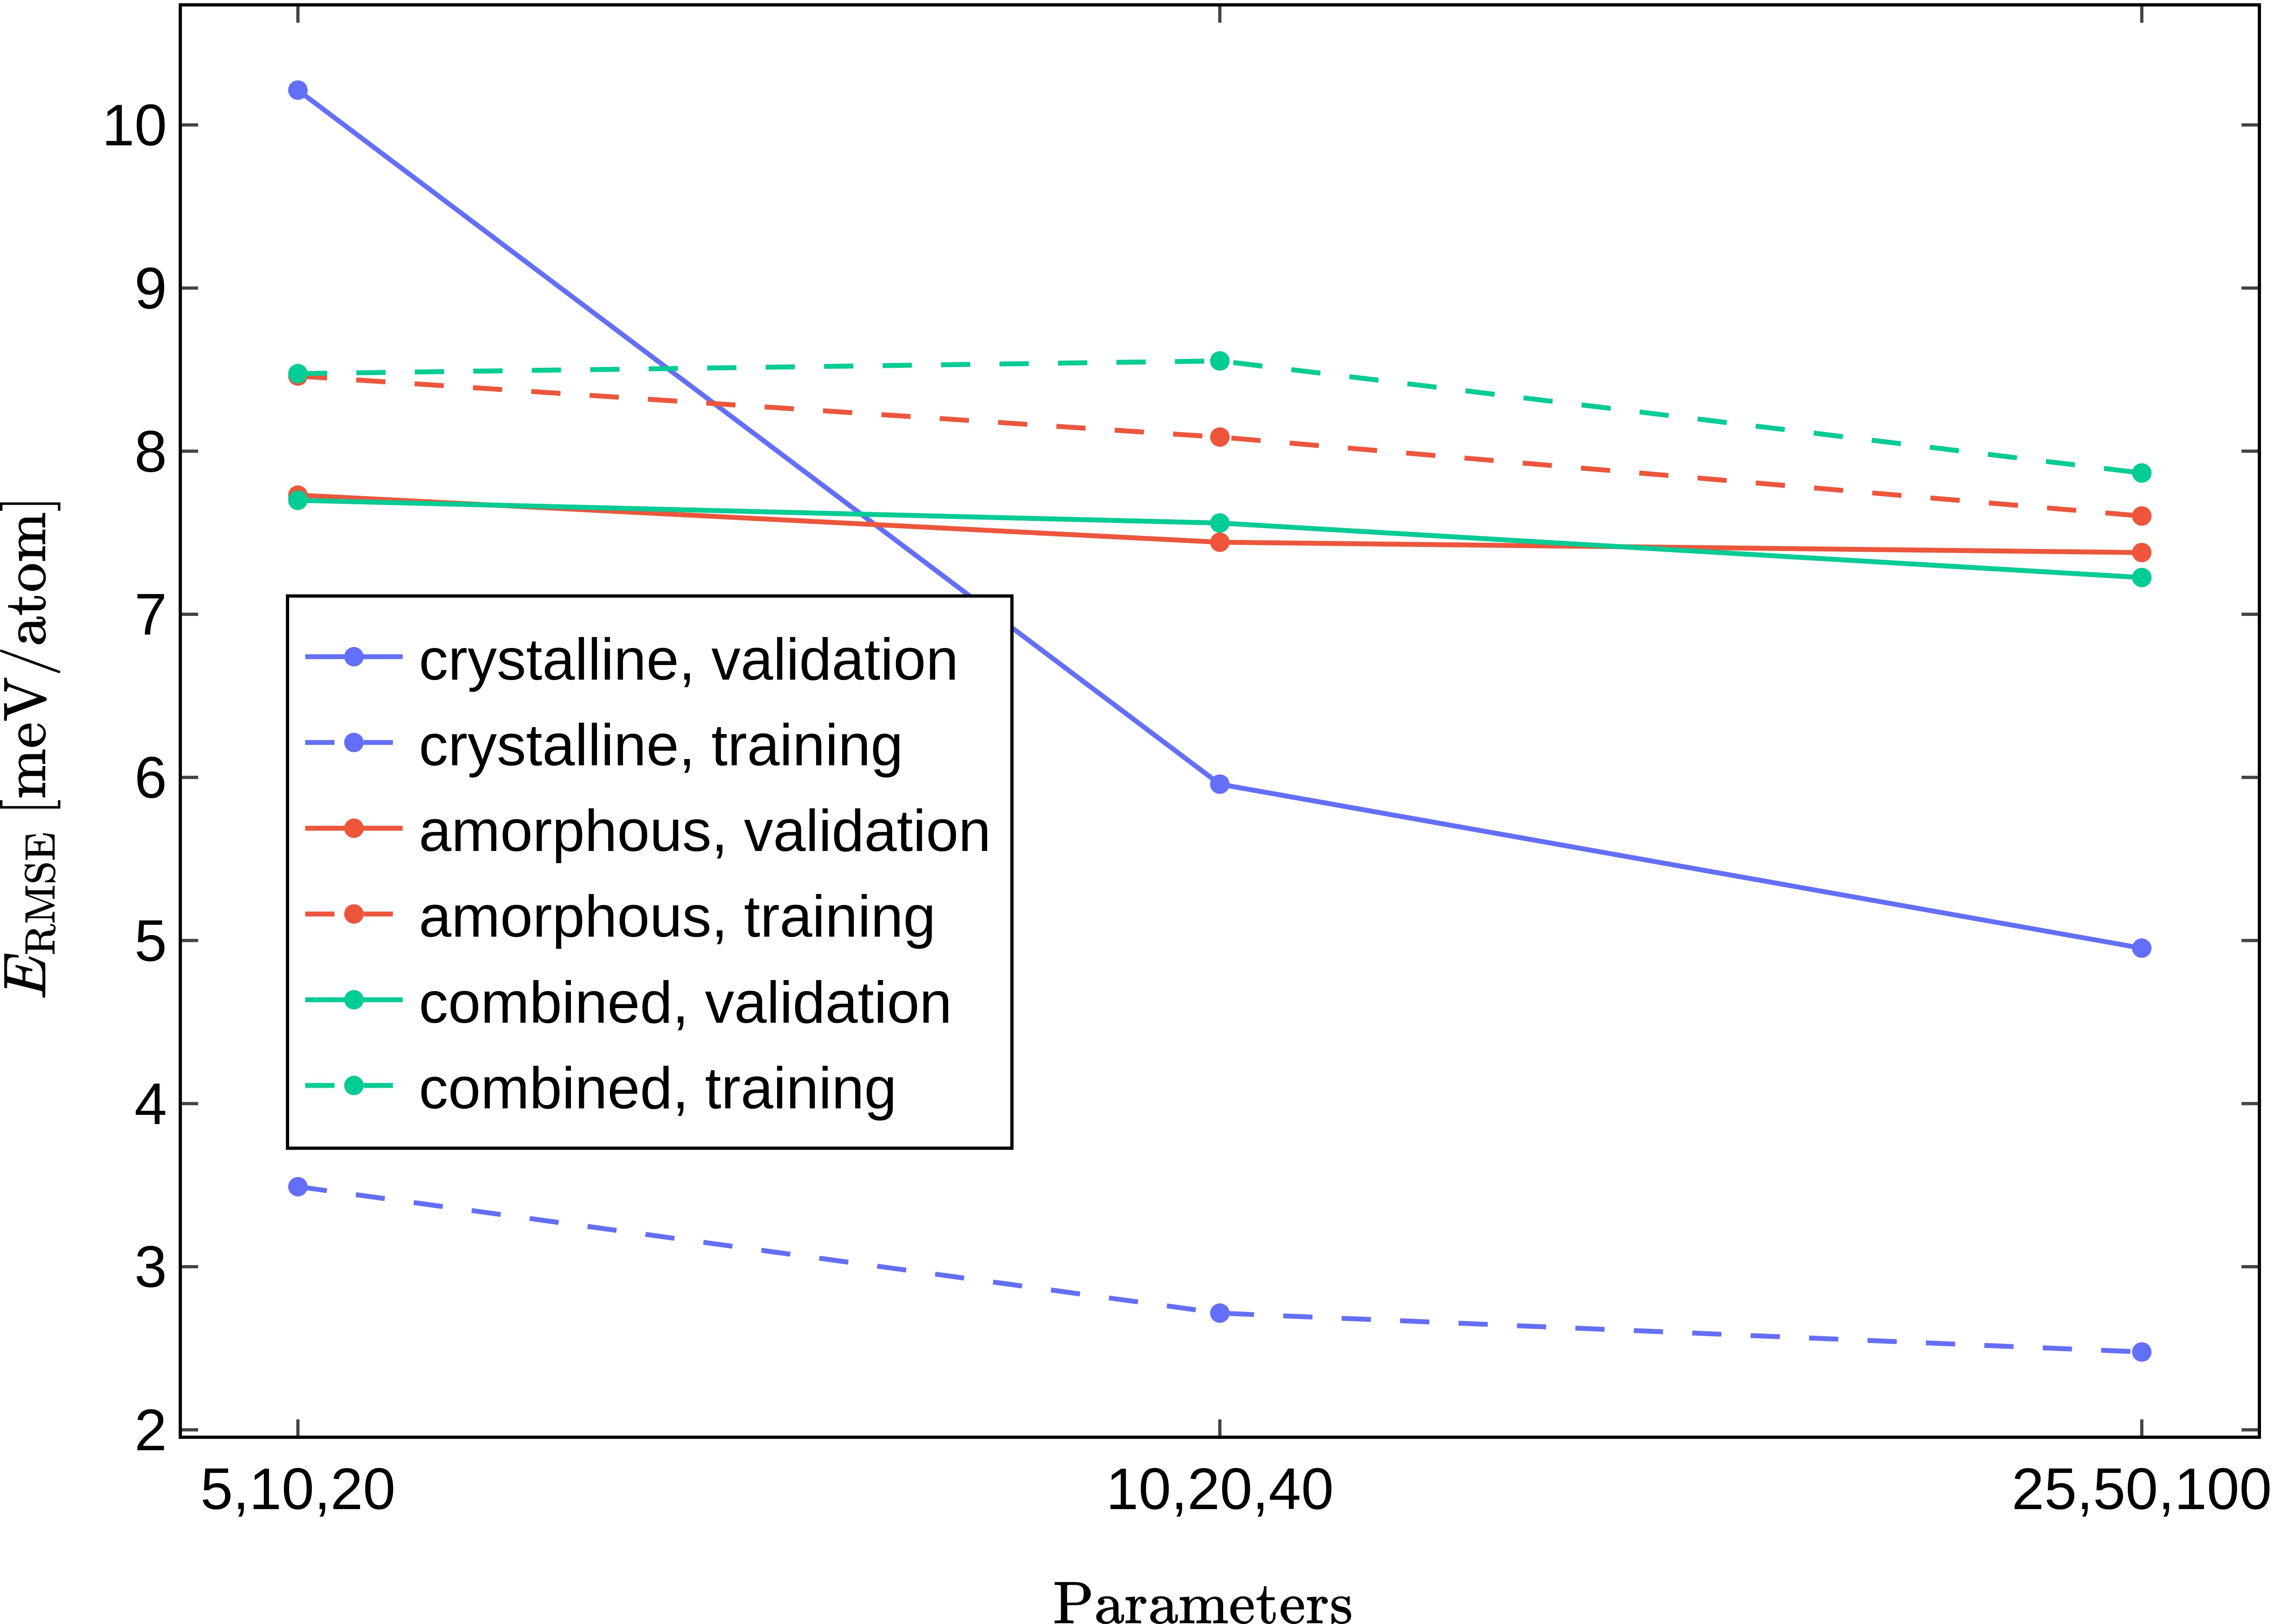
\includegraphics[width=.8\textwidth]{
      asset/descriptor_energy_error_evaluation.jpg
    }
  \end{center}
  \caption{Evaluation of energy errors for different descriptor neuron numbers.}
  \label{fig:descriptor_energy_error_evaluation}
\end{figure}

\begin{figure}
  \begin{center}
    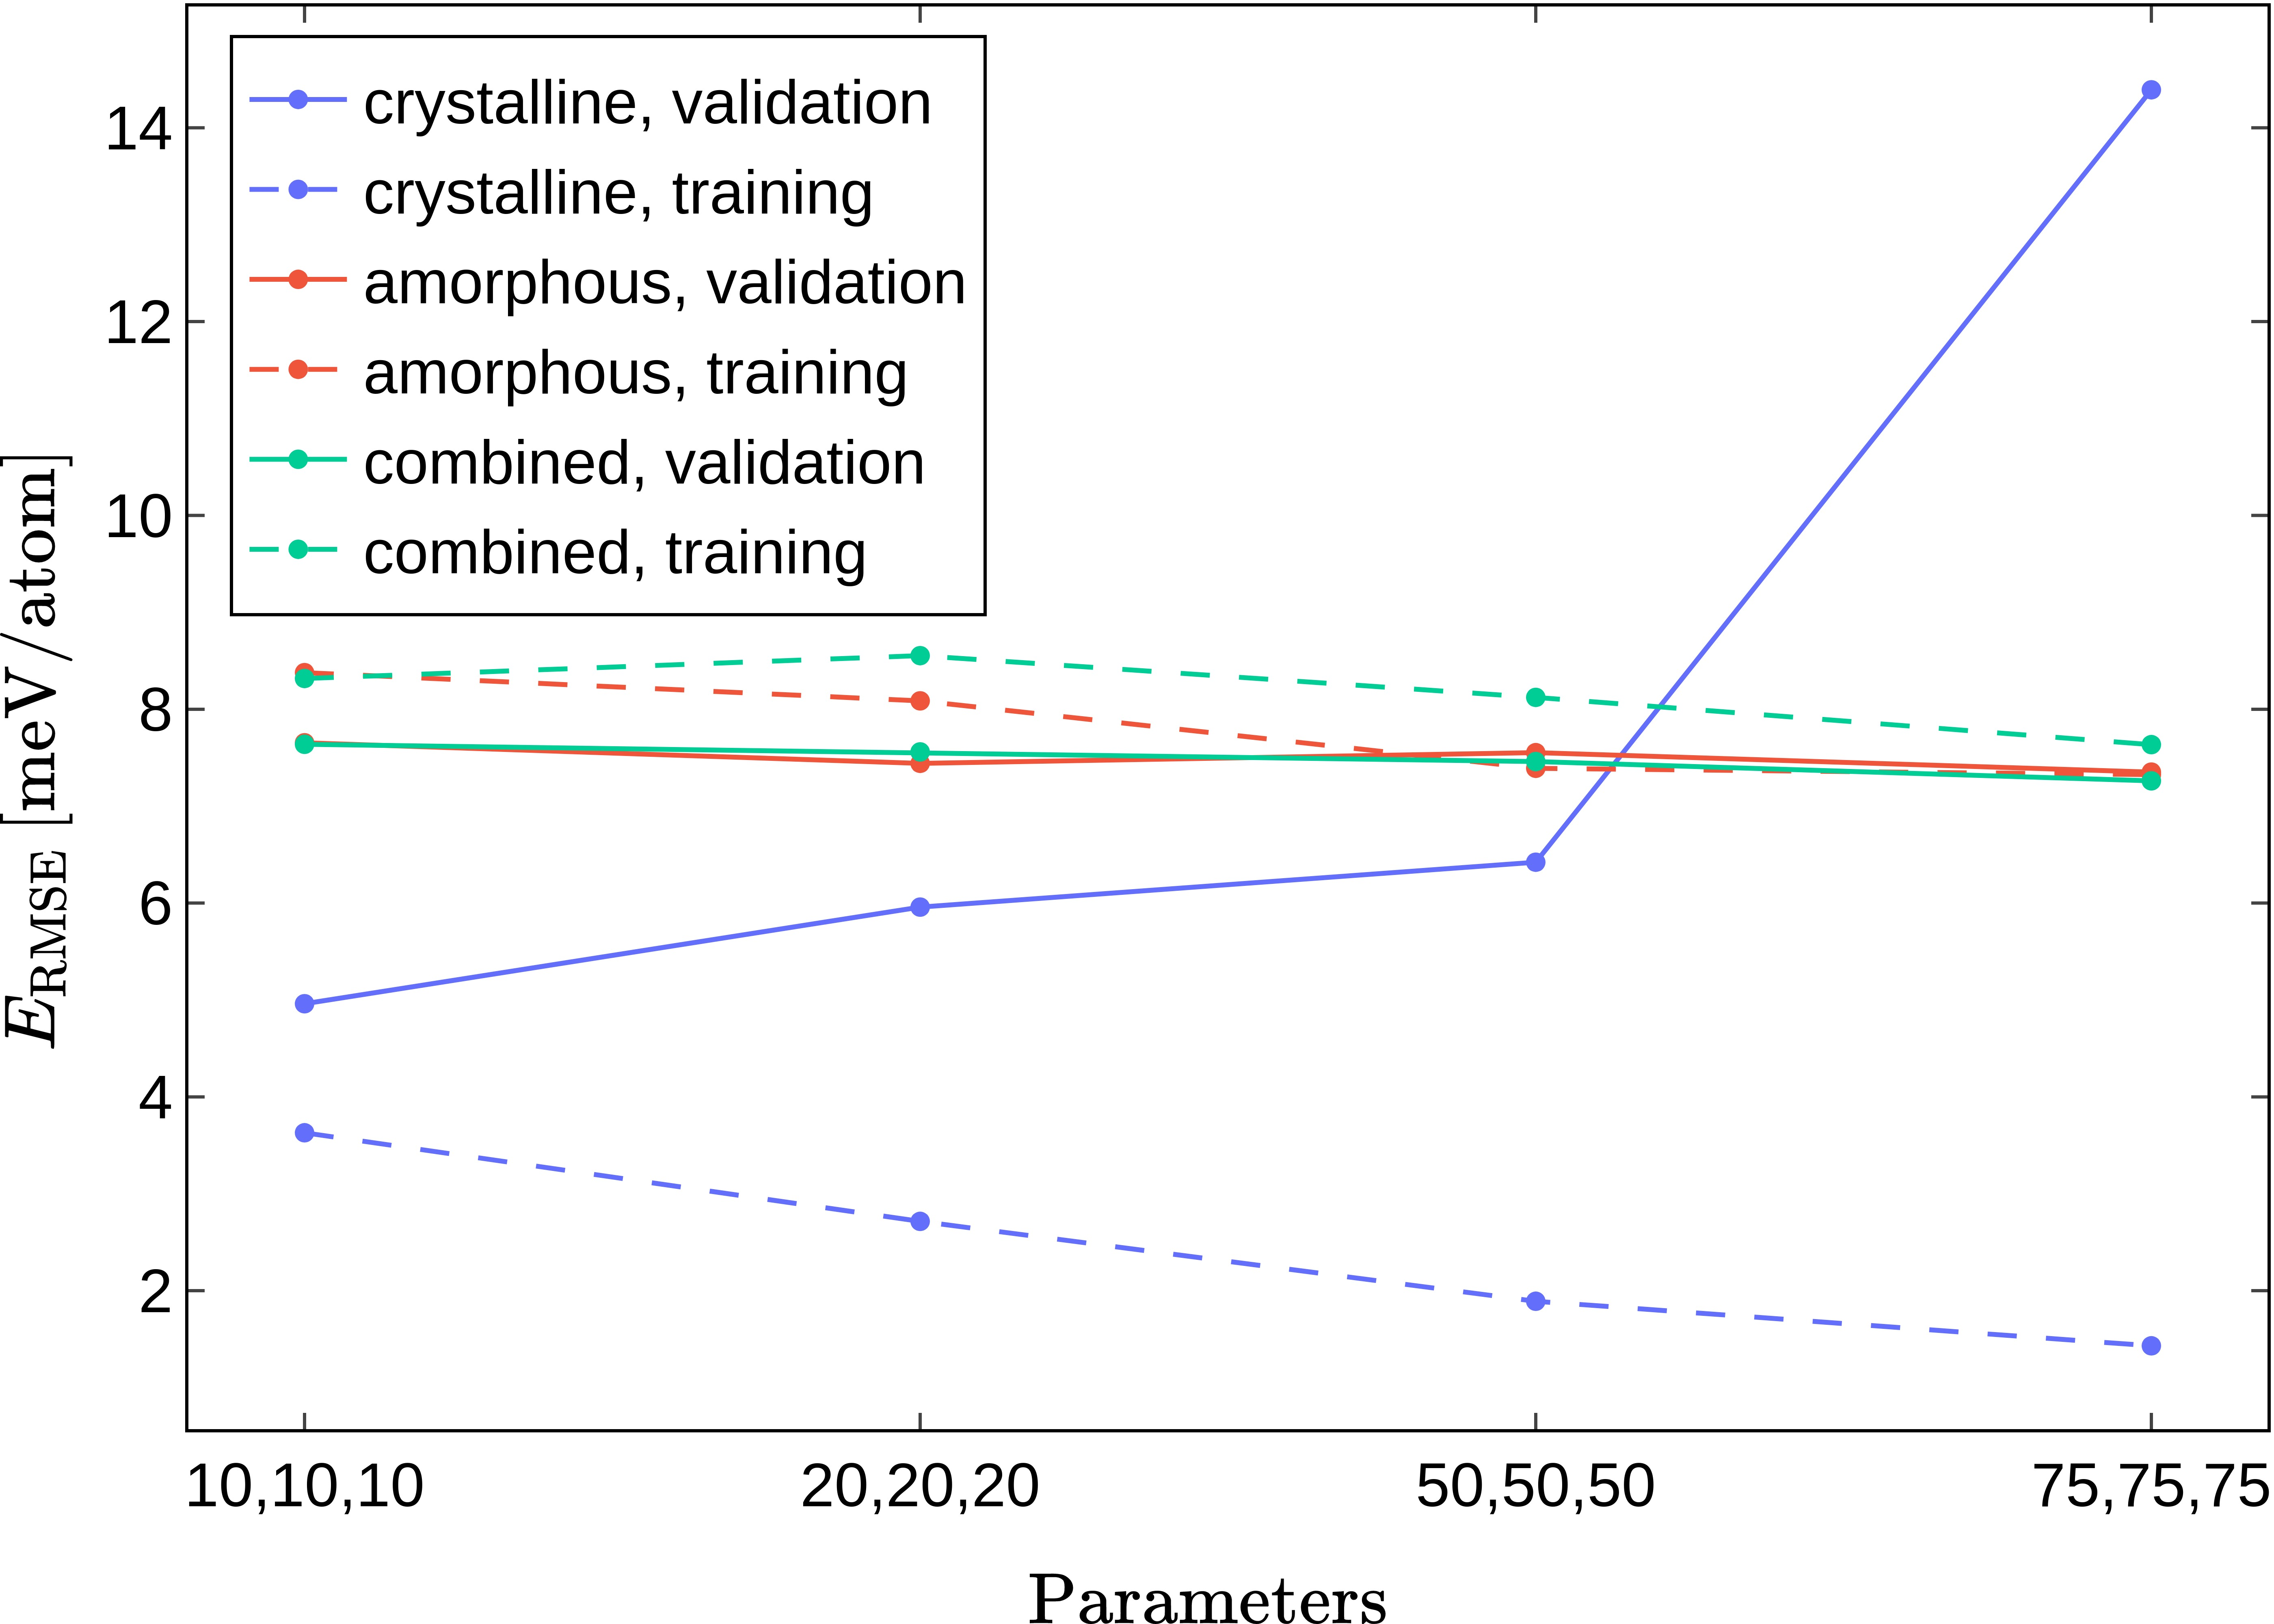
\includegraphics[width=.8\textwidth]{
      asset/fitting_energy_error_evaluation.jpg
    }
  \end{center}
  \caption{Evaluation of energy errors for different fitting neuron numbers.}
  \label{fig:fitting_energy_error_evaluation}
\end{figure}

\section{Inference Results}

The models \texttt{crystalline\_10,20,40d\_20,20,20f\_260222622s},
\texttt{cryst\-alline\_10,20,40d\_20,20,20f\_537693349s}, and
\texttt{crystalline\_10,20,\linebreak{}40d\_20,20,20f\_836424474s} were used to calculate
relaxation volume and bulk modulus for the Si diamond crystalline structure
at 0 K (cubic $\mathrm{F}\bar{\mathrm{d}}\mathrm{3m}$ space group). The
inference data with the fitted EOS models are shown below (figure
\ref{fig:crystalline_inference}). The calculated value for the relaxation
volume was $V_0 = 20.52 \pm 0.03$ \AA$^3$ and the calculated value for the
bulk modulus was
$B_{T_0} = 115 \pm 13 \, \mathrm{eV} \cdot \text{\AA}^{-3}$. Reference
materials for quantum mechanical calculations of the same structure give
values of $V_0 = 20.46$ \AA$^3$ and
$B_{T_0} = 98 \, \mathrm{GPa} \cdot \text{\AA}^{-3}$\cite{osti_1190959}.
Although the calculated values are not exactly in concordance with the
reference values, they are very close, and their relative errors are
only $\sim 0.3\%$ for the relaxation volume and $\sim 17 \%$ for the bulk
modulus. The values may differ firstly due to the different methodology and
configuration used for the qunatum mechanical calculations of the reference
and secondly due to the fact that the used models did not have enough training
data to converge exactly. Nonetheless, the results are very promising and show
that the models are able to predict the properties of the crystalline silicon
structure. This indicates a proper choice of the DNN hyperparameters. It is
also worth noting that the models were able to predict the properties of the
crystalline Si structure at 0 K even though they were only trained on data at
1500 K.

Comparing the inference results of the three models, it can be seen from the
figure \ref{fig:crystalline_inference} that the models give very similar
results near the equilibrium volume and start diverging significantly as more
strain is applied and the models are forced to extrapolate for unknown
conditions not seen in the learning data. To enhance the inference results,
more training data could be added for the volumes where the models diverge the
most.

\begin{figure}
  \begin{center}
    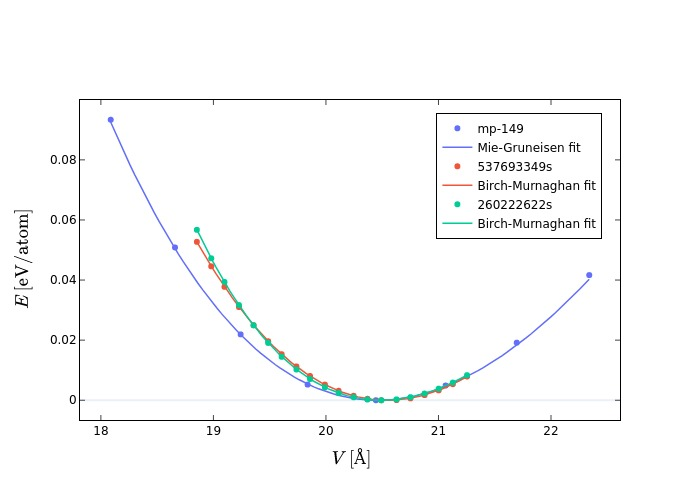
\includegraphics[width=.8\textwidth]{
      asset/crystalline_ev_curves.jpg
    }
  \end{center}
  \caption{Inference results for the Si diamond crystalline structure. The EV
  curves were shifted to have zero energy at the equilibrium volume for better
  comparison.}
  \label{fig:crystalline_inference}
\end{figure}

Next, the model \texttt{amorphous\_10,20,40d\_50,50,50f\_260222622s} was used
to calculate bulk modulus $B_0$ and volume thermal expansion coefficient
$\alpha_{V}$ for an amorphous silicon structure composed of 100 atoms with
density $\rho = 2.329 \, \mathrm{g} \cdot \mathrm{cm}^{-3}$. These material
properties were computed by fitting the Birch--Murnaghan EOS model to EV
curves calculated by the DNN at various temperatures. The results are shown in
figure \ref{fig:amorphous_inference}. The model seems to behave quite well at
temperatures up to 800 K. Above that temperature, the results start to produce
significant noise. Molecular dynamics at higher temperatures is more complex
and requires higher-quality predictions from the DNN to produce consistent
results. Most likely, our model is not able to produce such predictions
due to the low volume of the training data. Another reason could be that since
we only simulate 100 atoms in the amorphous structure, the statistical nature
of the simulation breaks down. These two problems could be solved by adding
more training data and simulating a larger number of atoms in the amorphous
structure. Another effect at play could be the fact that the amorphous Si
structure is not properly relaxed during the generation phase, as that would
require many more simulation steps. The structure is also being generated
using a different potential than the one used for the inference, which could
mean that even if the structure was properly relaxed, the relaxation state is
simply not compatible with the potential used for the inference. This could be
solved by using the same potential for both generation and inference and
by relaxing the structure for a longer time. Another problem could be that the
integration time used in the simulation is too large, which is also easily
solvable but would require more computational resources, which were not
available for this work.

\begin{figure}
  \begin{center}
    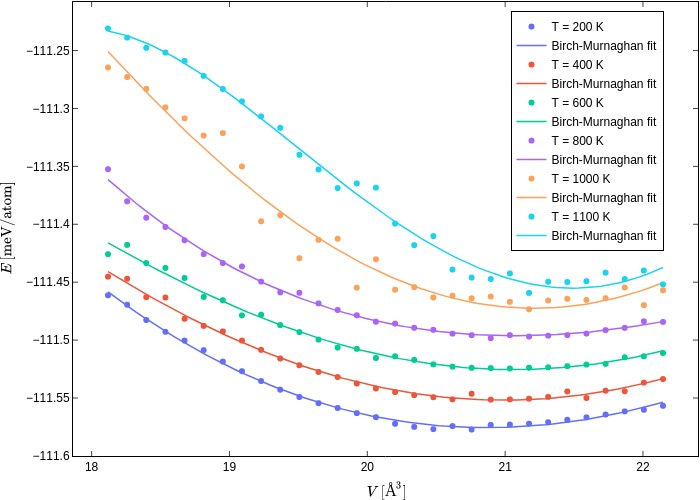
\includegraphics[width=.8\textwidth]{
      asset/amorphous_ev_curves.jpg
    }
  \end{center}
  \caption{Inference results for the Si amorphous structure at various
  temperatures.}
  \label{fig:amorphous_inference}
\end{figure}

\begin{figure}
  \begin{center}
    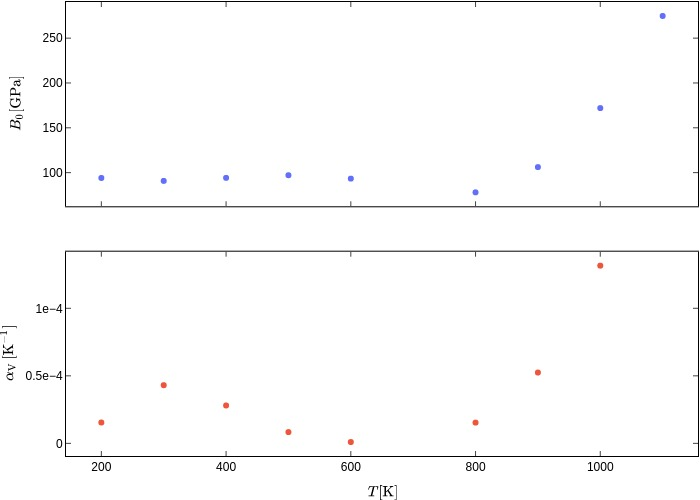
\includegraphics[width=.8\textwidth]{
      asset/amorphous_properties.jpg
    }
  \end{center}
  \caption{The dependence of the bulk modulus $B_0$ and volumetric thermal
  expansion coefficient $\alpha_V$ on temperature $T$ for the amorphous
  silicon structure.}
  \label{fig:amorphous_properties}
\end{figure}

Experimental values of the Young modulus $\mathcal{E}$ and the Poisson's ratio
$\nu$ for polycrystalline silicon material are $\sim 170 \, \mathrm{GPa}$ and
$\sim 0.22$, respectively \cite{Freund_Suresh_2003}. The relation between the
bulk modulus $B_0$, the Young modulus $\mathcal{E}$, and the Poisson's ratio
$\nu$ for an isotropic material is
\begin{equation}
  B_0 = \frac{\mathcal{E}}{3(1 - 2\nu)}.
\end{equation}
Using this formula, we can calculate the bulk modulus of polysilicon $B_0$ to
be $\sim 101 \, \mathrm{GPa}$. The modeled bulk modulus $B_0$ for the
amorphous silicon used in this work is
$\sim 94 \, \mathrm{GPa}$ at $T = 200 \, \mathrm{K}$,
$\sim 91 \, \mathrm{GPa}$ at $T = 300 \, \mathrm{K}$,
$\sim 94 \, \mathrm{GPa}$ at $T = 400 \, \mathrm{K}$,
and $\sim 78 \, \mathrm{GPa}$ at $T = 800 \, \mathrm{K}$.

The linear expansion coefficient $\beta$ for an amorphous Si is experimentally
measured to be $\sim 3.6 \cdot 10^{-6} \, \mathrm{K}^{-1}$ at
$T = 318.15 \, \mathrm{K}$, $\sim 3.0 \cdot 10^{-6} \, \mathrm{K}^{-1}$ at
$T = 418.15 \, \mathrm{K}$ \cite{TAKIMOTO2002314}. The relation between the
linear expansion coefficient $\beta$ and the volumetric expansion coefficient
$\alpha_V$ is
\begin{equation}
  \alpha_V = 3 \cdot \beta.
\end{equation}
Converting these values of the linear expansion coefficient $\beta$ to the
volumetric expansion coefficient $\alpha_V$ we get
$\sim 1.1 \cdot 10^{-5} \, \mathrm{K}^{-1}$ at $T = 318.15 \, \mathrm{K}$ and
$\sim 0.9 \cdot 10^{-5} \, \mathrm{K}^{-1}$ at $T = 418.15 \, \mathrm{K}$.
Our models arrived at values for $\alpha_V$ to be
$\sim 4.3 \cdot 10^{-5} \, \mathrm{K}^{-1}$ at
$T = 350 \, \mathrm{K}$, $\sim 2.8 \cdot 10^{-5} \, \mathrm{K}^{-1}$ at
$T = 450 \, \mathrm{K}$. The inference results for the bulk modulus $B_0$ had
relative errors of $\sim 10 \%$ and their quality was on par with the quality
of the inference results for the crystalline silicon except for outliers
($T = 700 \, \mathrm{K}$) and for too high temperatures
($T > 800 \, \mathrm{K}$). The results for the volumetric thermal expansion
coefficient unfortunately ended with significant relative errors of
$\sim 290 \%$. The very high relative errors for the volumetric
thermal expansion coefficient $\alpha_V$ are most likely caused by the fact
that the calculations depend mostly on correct predictions of the relaxation
volume $V_0$ of the amorphous structure at various temperatures. Even though
the DNN models were able to predict the volume $V_0$ of the crystalline
structure very well, the predictions for the amorphous structure are by nature
more uncertain as they depend on proper relaxation of the generated structure
and are thus sensitive to the choice of the potentials used in the
various steps of the computation process (OpenMX pseudopotentials used for
the training data generation, OpenKIM potentials used for the amorphous
structure generation and relaxation, and the DeepMD potential itself used for
the MD simulation). Furthermore, as has already been mentioned, the size of
the amorphous structure used in the inference is relatively small, which
breaks the statistical nature of the system and causes the results to be noisy
at higher temperatures. It's also obvious that the results for the $\alpha_V$
are much more error-prone than the results for the $B_0$ as the former is
calculated from just one value (the volume $V_0$) while the latter is given by
the slope of the EV curve, which is much more resilient to noise. These errors
are, however, just a rough estimate, as the experimental values for the
amorphous silicon are obtained for vastly different conditions (the material
is not completely amorphous but polycrystalline, the temperatures and
pressures are different, the measurement methods are different, etc.) than the
ones calculated in this work. The calculated values are more uncertain the
higher the temperature is, as can be clearly seen from the noise in the EV
curves for higher temperatures in figure \ref{fig:amorphous_inference}. This
is expected, as the molecular dynamics is more complicated at higher
temperatures and the DNN models are forced to extrapolate more. The results
are nonetheless very promising and show that the models are able to predict
the properties of the amorphous silicon structure.

\chapter{Conclusion}

This work used the DeepMD methodology to demonstrate the viability and
efficiency of machine learning potentials for performing molecular dynamics
and calculating the material properties of both crystalline and amorphous
materials. We have trained a wide variety of DNN models to show how
hyperparameter selection affects their inference accuracy. We then used the
best-performing models to perform molecular dynamics simulations of crystalline and amorphous silicon. Subsequently, we
used the data from the molecular dynamics simulations to compute the
equilibrium volume $V_0$, the bulk modulus $B_0$, and the volumetric thermal
expansion coefficient $\alpha_V$ of silicon. The results from the machine
learning models were very promising and showed that we can get quite accurate
results with relative errors of $\sim 0.3\%$ for the relaxation volume $V_0$
of crystalline silicon, $\sim 17 \%$ for the bulk modulus $B_0$ of crystalline
silicon, compared to different third-party DFT calculations. A significantly
worse performance was observed for amorphous silicon, where the relative error
was compared to the experimental data, with $\sim 90 \%$ error for the bulk modulus.
It was noted that our modeled data was too noisy for calculating the volumetric
thermal expansion coefficient $\alpha_V$ of amorphous silicon, but we believe that this
was mostly due to the shortcomings of the specific settings of our methodology
caused by a lack of computational resources and time, not by the inherent conceptual flaws in
the DNN modeling approach. We note that the accuracy of the results can be
drastically improved by using larger atomic systems and bigger training data sets,
and that the quality and size of the training data sets are the most important factors limiting the
model prediction accuracy. We also note that this may be quite problematic as
quality training data can only be obtained with computationally expensive
quantum mechanical simulations, which is the main bottleneck for the DeepMD
methodology.

Future work should focus on improving the quality of the training data sets,
making use of methodologies for generating training data on the fly (e.g., by
using the active learning approach), comparing the DeepMD methodology with
alternative machine learning implementations, or accelerating the current DeepMD
protocol presented in this work by moving to GPU-based learning and inference.


\printbibliography[heading=bibintoc]
\makeatletter\thesis@blocks@clear\makeatother
\phantomsection
\addcontentsline{toc}{chapter}{\indexname}
\printindex

\end{document}
